\documentclass[12pt,a4paper]{article}

% ================== PACKAGES ==================
\usepackage[margin=2.54cm]{geometry}
\usepackage[utf8]{inputenc}
\usepackage[T5]{fontenc}
\usepackage[vietnamese]{babel}
\usepackage{lmodern}
\usepackage{setspace}
\usepackage{booktabs}
\usepackage{array}
\usepackage{tabularx}
\usepackage{longtable}
\usepackage{graphicx}
\usepackage{xcolor}
\usepackage{hyperref}
\usepackage{listings}
\usepackage{amsmath}
\usepackage{amssymb}
\usepackage{enumitem}
\usepackage{fancyhdr}
\usepackage{titlesec}
\usepackage{xurl}
\usepackage{float}
\usepackage{tocloft}
\usepackage{csquotes}
\usepackage{tikz}
\usepackage{caption}

\usetikzlibrary{
    arrows.meta,
    positioning,
    calc,
    matrix,
    decorations.pathreplacing
}

% ================== REFERENCES ==================
\usepackage[
    backend=biber,
    style=ieee,
    sorting=none
]{biblatex}

\addbibresource{references.bib}

% ================== FONT & SPACING ==================
\onehalfspacing
\setlength{\emergencystretch}{3em}

% ================== PARAGRAPH FORMAT ==================
\setlength{\parindent}{1.25cm}
\setlength{\parskip}{0pt}

% ================== HYPERREF SETUP ==================
\hypersetup{
    colorlinks=true,
    linkcolor=blue,
    citecolor=blue,
    urlcolor=cyan,
    pdftitle={
        Jailbreaking Large Language Models and Agentic Systems:
        Attacks, Defenses, and Evaluations
    },
    pdfauthor={Group 07}
}

% ================== HEADER & FOOTER ==================
\pagestyle{fancy}
\fancyhf{}
\lhead{ICML 2025 Tutorial}
\rhead{Jailbreaking LLMs}
\rfoot{Trang \thepage}

\setlength{\headheight}{15pt}

% ================== TITLE FORMAT ==================
\titleformat{\section}
    {\Large\bfseries}
    {\thesection}
    {1em}
    {}

\titleformat{\subsection}
    {\large\bfseries}
    {\thesubsection}
    {1em}
    {}

\titleformat{\subsubsection}
    {\normalsize\bfseries}
    {\thesubsubsection}
    {1em}
    {}

% ================== LISTING SETUP ==================
\lstset{
    basicstyle=\ttfamily\small,
    breaklines=true,
    frame=single,
    numbers=left,
    numberstyle=\tiny,
    keywordstyle=\color{blue},
    commentstyle=\color{gray},
    stringstyle=\color{red},
    showstringspaces=false,
    tabsize=4
}

% ================== CUSTOM COMMANDS ==================
\newcommand{\abbr}[2]{#1 & #2 \\}
\newcommand{\method}[1]{\textsc{#1}}
\newcommand{\modelname}[1]{\texttt{#1}}

% ================== VIETNAMESE NAMES ==================
\renewcommand{\contentsname}{Mục lục}
\renewcommand{\listfigurename}{Danh mục hình vẽ}
\renewcommand{\listtablename}{Danh mục bảng}
\renewcommand{\figurename}{Hình}
\renewcommand{\tablename}{Bảng}
\renewcommand{\appendixname}{Phụ lục}

% ================== DOCUMENT ==================
\begin{document}

% ================== TITLE PAGE ==================
\begin{titlepage}
\begin{center}

{\large
ĐẠI HỌC QUỐC GIA THÀNH PHỐ HỒ CHÍ MINH\\
TRƯỜNG ĐẠI HỌC KHOA HỌC TỰ NHIÊN\\
KHOA CÔNG NGHỆ THÔNG TIN
}\\[2.5cm]


\includegraphics[width=4cm]{logo-khtn.png}\\[1.2cm]

{\color{blue}\LARGE\textbf{ĐỒ ÁN 3}}\\[0.6cm]

{\LARGE\textbf{
JAILBREAKING LARGE LANGUAGE MODELS AND AGENTIC SYSTEMS
}}\\[2.5cm]


\begin{tabular}{ll}
\textbf{Mã số sinh viên} & \textbf{Họ và tên} \\[0.2cm]
23120245 & Nguyễn Quang Duy \\
23120258 & Lưu Trọng Hiếu \\
23120260 & Văn Đình Hiếu \\
\end{tabular}

\vfill

\begin{tabular}{ll}
\textbf{Giảng viên hướng dẫn:}
    & TS. Bùi Tiến Lên \\
    & ThS. Lê Nhựt Nam \\
\end{tabular}

\vfill


\vspace{0.5cm}
\textbf{Môn học:} & Nhập môn Học máy \\
\textbf{Thành phố Hồ Chí Minh -- 2026}

\end{center}
\end{titlepage}

% ================== FRONT MATTER ==================
\pagenumbering{roman}
\setcounter{page}{1}

% ================== ABSTRACT ==================
\section*{Tóm tắt}
\addcontentsline{toc}{section}{Tóm tắt}

Sự phát triển nhanh chóng của các mô hình ngôn ngữ lớn
(Large Language Models -- LLMs) đã thúc đẩy việc ứng dụng trí tuệ
nhân tạo vào nhiều lĩnh vực như trợ lý hội thoại, hỗ trợ lập trình,
tìm kiếm thông tin, tự động hóa quy trình và các hệ thống tác tử có
khả năng sử dụng công cụ. Cùng với sự mở rộng về năng lực, vấn đề
bảo đảm mô hình tuân thủ các nguyên tắc an toàn và không tạo ra hành
vi ngoài mong muốn trở thành một yêu cầu quan trọng. Tuy nhiên, các
cơ chế căn chỉnh an toàn hiện nay vẫn có thể bị vượt qua bởi các kỹ
thuật jailbreaking, trong đó đầu vào được xây dựng hoặc tối ưu nhằm
khiến mô hình không tuân theo những ràng buộc an toàn đã được thiết lập.

Báo cáo này tổng hợp nội dung của tutorial
\textit{Jailbreaking LLMs and Agentic Systems: Attacks, Defenses,
and Evaluations}. Trước hết, báo cáo trình bày kiến thức nền về mô hình
ngôn ngữ lớn, instruction tuning, alignment và threat model trong
nghiên cứu an toàn mô hình. Tiếp theo, các phương pháp jailbreak được
hệ thống hóa theo quyền truy cập của kẻ tấn công, mức độ tự động hóa,
cơ chế tìm kiếm và số lượt tương tác. Các hướng phòng thủ được phân
loại theo vị trí triển khai, bao gồm xử lý đầu vào, điều chỉnh mô hình,
phòng thủ trong quá trình suy luận, kiểm duyệt đầu ra và bảo vệ ở cấp
hệ thống.

Báo cáo đồng thời khảo sát các benchmark và tiêu chí đánh giá như
Attack Success Rate, refusal rate, over-refusal rate và benign utility.
Ngoài các chatbot dựa trên văn bản, báo cáo mở rộng phân tích sang
agentic systems và robot được điều khiển bởi LLM, nơi một cuộc tấn công
thành công có thể không chỉ thay đổi nội dung phản hồi mà còn tác động
đến quá trình lập kế hoạch, gọi công cụ và thực hiện hành động. Cuối
cùng, nhóm trình bày thiết kế demo thực nghiệm nhằm so sánh một số
phương pháp tấn công và phòng thủ trong môi trường kiểm soát, đồng thời
phân tích sự đánh đổi giữa độ an toàn, khả năng hữu ích và chi phí tính
toán của hệ thống.

\textbf{Từ khóa:}
mô hình ngôn ngữ lớn, jailbreaking, alignment, an toàn trí tuệ nhân tạo,
adversarial attack, jailbreak defense, automated red teaming,
agentic systems.

\newpage

% ================== TABLE OF CONTENTS ==================
\tableofcontents
\newpage

% ================== ABBREVIATIONS ==================
\section*{Danh mục từ viết tắt}
\addcontentsline{toc}{section}{Danh mục từ viết tắt}

\begin{center}
\begin{tabularx}{\textwidth}{
    >{\bfseries}p{0.20\textwidth}
    X
}
\toprule
\textbf{Từ viết tắt} & \textbf{Ý nghĩa} \\
\midrule

AI
& Artificial Intelligence -- Trí tuệ nhân tạo \\

API
& Application Programming Interface -- Giao diện lập trình ứng dụng \\

ASR
& Attack Success Rate -- Tỷ lệ tấn công thành công \\

GCG
& Greedy Coordinate Gradient \\

ICML
& International Conference on Machine Learning \\

LLM
& Large Language Model -- Mô hình ngôn ngữ lớn \\

MLLM
& Multimodal Large Language Model -- Mô hình ngôn ngữ lớn đa phương thức \\

PAIR
& Prompt Automatic Iterative Refinement \\

ReAct
& Reasoning and Acting \\

RLHF
& Reinforcement Learning from Human Feedback \\

SFT
& Supervised Fine-Tuning \\

TAP
& Tree of Attacks with Pruning \\

TDC
& Trojan Detection Challenge \\

\bottomrule
\end{tabularx}
\end{center}

\newpage

% ================== LIST OF FIGURES ==================
\phantomsection
\addcontentsline{toc}{section}{Danh mục hình vẽ}
\listoffigures
\newpage

% ================== LIST OF TABLES ==================
\phantomsection
\addcontentsline{toc}{section}{Danh mục bảng}
\listoftables
\newpage

% ================== MAIN MATTER ==================
\pagenumbering{arabic}
\setcounter{page}{1}
\setcounter{figure}{0}
\setcounter{table}{0}

\section{Giới thiệu}
\label{sec:introduction}

\subsection{Bối cảnh nghiên cứu}
\label{subsec:introduction-context}

Trong những năm gần đây, các mô hình ngôn ngữ lớn
(Large Language Models -- LLMs) đã trở thành thành phần quan trọng trong
nhiều ứng dụng như trợ lý hội thoại, hỗ trợ lập trình, tìm kiếm thông tin,
phân tích tài liệu và tự động hóa quy trình. Khi được kết hợp với bộ nhớ,
khả năng lập kế hoạch và cơ chế gọi công cụ, LLM không chỉ sinh phản hồi
dạng văn bản mà còn có thể đóng vai trò như bộ điều khiển của các hệ thống
tác tử thông minh, thường được gọi là \textit{agentic systems}.

Sự mở rộng này làm tăng đáng kể yêu cầu về an toàn. Một chatbot truyền
thống chủ yếu tạo ra phản hồi văn bản, trong khi một agentic system có thể
truy xuất dữ liệu, gọi API, thao tác trên tệp hoặc tương tác với môi trường
bên ngoài. Do đó, một hành vi không an toàn trong hệ thống tác tử có thể
dẫn đến hậu quả nghiêm trọng hơn so với một phản hồi văn bản không phù hợp.

Để giảm thiểu rủi ro, các LLM hiện đại thường được căn chỉnh bằng nhiều
kỹ thuật như supervised fine-tuning, preference optimization, Reinforcement
Learning from Human Feedback (RLHF) và safety fine-tuning. Bên cạnh đó,
hệ thống triển khai còn có thể sử dụng system prompt, bộ lọc đầu vào, bộ
phân loại an toàn và kiểm duyệt đầu ra. Tuy nhiên, các cơ chế này chưa tạo
ra bảo đảm tuyệt đối. Nhiều nghiên cứu cho thấy hành vi từ chối của mô hình
vẫn có thể bị làm suy yếu bởi các đầu vào được thiết kế có chủ đích, gọi
chung là \textit{jailbreak attacks}
\cite{yi2024jailbreak,zou2023universal,chao2023pair}.

\subsection{Bài toán jailbreaking}
\label{subsec:jailbreaking-problem}

Trong phạm vi báo cáo này, jailbreaking được hiểu là quá trình xây dựng
hoặc tối ưu đầu vào nhằm khiến một mô hình đã được căn chỉnh an toàn tạo
ra hành vi trái với các ràng buộc mà nhà phát triển đặt ra. Kẻ tấn công
không nhất thiết phải thay đổi tham số hoặc dữ liệu huấn luyện của mô hình;
trong nhiều trường hợp, họ chỉ có quyền gửi truy vấn và quan sát phản hồi
của hệ thống.

Một cách khái quát, hệ thống LLM có thể được biểu diễn bởi

\begin{equation}
    y = F_{\theta}(x, s, c),
    \label{eq:aligned-llm-output}
\end{equation}

trong đó $x$ là yêu cầu của người dùng, $s$ là system prompt hoặc chính
sách hệ thống, $c$ là ngữ cảnh bổ sung và $F_{\theta}$ là mô hình với tham
số $\theta$. Jailbreak attack tìm một phép biến đổi $\mathcal{T}$ sao cho

\begin{equation}
    x' = \mathcal{T}(x),
    \label{eq:jailbreak-transformation}
\end{equation}

trong đó $x'$ vẫn giữ mục tiêu ngữ nghĩa của yêu cầu ban đầu nhưng khiến
đầu ra của hệ thống không còn thuộc tập phản hồi an toàn:

\begin{equation}
    F_{\theta}(x', s, c)
    \notin
    \mathcal{Y}_{\mathrm{safe}}.
    \label{eq:jailbreak-objective}
\end{equation}

Jailbreaking có liên hệ với prompt injection nhưng không hoàn toàn đồng
nhất. Jailbreaking thường tập trung vào việc vượt qua các ràng buộc an
toàn của mô hình, trong khi prompt injection nhắm đến việc làm thay đổi
thứ tự ưu tiên hoặc luồng thực thi chỉ dẫn trong một ứng dụng dùng LLM.
Trong agentic systems, hai dạng rủi ro này có thể xuất hiện đồng thời.

\subsection{Mục tiêu báo cáo}
\label{subsec:objectives}

Báo cáo này được xây dựng dựa trên tutorial ICML 2025
\textit{Jailbreaking LLMs and Agentic Systems: Attacks, Defenses, and
Evaluations} \cite{jailbreak_tutorial_2025}. Mục tiêu chính là hệ thống hóa
các nội dung nền tảng về jailbreaking, bao gồm threat model, phương pháp
tấn công, phương pháp phòng thủ, cách đánh giá và sự mở rộng của bài toán
sang agentic systems.

Cụ thể, báo cáo tập trung vào các mục tiêu sau:

\begin{enumerate}[label=\textbf{M\arabic*.}, leftmargin=2.2cm]
    \item Trình bày nền tảng về LLM, instruction tuning, safety alignment
    và threat model.
    \item Hệ thống hóa các nhóm jailbreak attacks theo cơ chế xây dựng
    prompt, quyền truy cập và số lượt tương tác.
    \item Phân tích các lớp phòng thủ đối với jailbreak ở cấp đầu vào,
    mô hình, suy luận, đầu ra và toàn hệ thống.
    \item Trình bày các metric, evaluator và benchmark thường dùng để
    đánh giá jailbreak.
    \item Làm rõ sự khác biệt giữa jailbreak trên chatbot và jailbreak
    trên agentic systems.
    \item Xây dựng demo thực nghiệm trong môi trường kiểm soát để minh họa
    attack--defense pipeline.
\end{enumerate}

\subsection{Phạm vi báo cáo}
\label{subsec:report-scope}

Báo cáo tập trung vào jailbreaking tại thời điểm suy luận đối với các LLM
đã được huấn luyện và triển khai. Nội dung chính bao gồm jailbreak trên LLM
sinh văn bản, white-box và black-box attacks, single-turn và multi-turn
attacks, automated red teaming, các lớp phòng thủ, benchmark đánh giá,
prompt injection trong agentic systems và jailbreaking đối với robot được
điều khiển bởi LLM.

Báo cáo không nhằm bao quát toàn bộ lĩnh vực adversarial machine learning.
Các chủ đề như data poisoning, model extraction, membership inference,
backdoor trong huấn luyện và tấn công hạ tầng chỉ được nhắc đến khi cần
phân biệt với jailbreaking. Phần demo được thực hiện trong môi trường kiểm
soát, với mục tiêu nghiên cứu và đánh giá an toàn.

\subsection{Cấu trúc báo cáo}
\label{subsec:report-structure}

Phần còn lại của báo cáo được tổ chức như sau. Chương~\ref{sec:background}
trình bày kiến thức nền về LLM, instruction tuning, safety alignment và
threat model. Chương~\ref{sec:jailbreak-attacks} hệ thống hóa các phương
pháp jailbreak, bao gồm manual attacks, obfuscation, multi-turn jailbreak,
white-box optimization, black-box automated jailbreak, transferability và
adaptive attacks. Chương~\ref{sec:jailbreak-defenses} phân tích các phương
pháp phòng thủ như input filtering, adversarial training, inference-time
defenses, output moderation, guard models và defense-in-depth.

Chương~\ref{sec:evaluation-benchmarks} trình bày các phương pháp đánh giá
và benchmark, bao gồm Attack Success Rate, refusal, harmfulness, utility,
over-refusal, human evaluation, classifier-based evaluation,
LLM-as-a-judge, AdvBench, HarmBench và JailbreakBench. Chương~\ref{sec:agentic-systems}
mở rộng bài toán sang agentic systems, bao gồm prompt injection, tool-use
attacks, memory poisoning, LLM-controlled robots và agent-specific defenses.
Chương~\ref{sec:related-papers} phân tích các công trình tiêu biểu được
tutorial đề cập. Chương~\ref{sec:experiments} mô tả demo, thiết lập thực
nghiệm, kết quả và phân tích lỗi. Chương~\ref{sec:discussion} thảo luận
các hạn chế, safety--utility trade-off, attack--defense arms race và hướng
nghiên cứu tương lai. Cuối cùng, Chương~\ref{sec:conclusion} tổng kết các
nội dung chính của báo cáo.
\section{Kiến thức nền}
\label{sec:background}

Chương này trình bày các khái niệm nền tảng cần thiết để phân tích
jailbreak attacks, jailbreak defenses và phương pháp đánh giá độ an toàn
của các mô hình ngôn ngữ lớn. Nội dung tập trung vào cách LLM sinh phản
hồi, quá trình căn chỉnh mô hình, thứ bậc chỉ dẫn, threat model, các khái
niệm an toàn liên quan và sự khác biệt giữa chatbot với agentic systems.

\subsection{Mô hình ngôn ngữ lớn}
\label{subsec:large-language-models}

Mô hình ngôn ngữ lớn (Large Language Model -- LLM) là mô hình học máy
được huấn luyện trên lượng lớn dữ liệu văn bản để học phân phối xác suất
của ngôn ngữ. Với một chuỗi token đầu vào

\begin{equation}
    x = (x_1, x_2, \ldots, x_n),
\end{equation}

mô hình tự hồi quy ước lượng xác suất của token tiếp theo dựa trên các
token đã xuất hiện trước đó:

\begin{equation}
    P_{\theta}(x_{n+1} \mid x_1, x_2, \ldots, x_n),
    \label{eq:next-token-probability}
\end{equation}

trong đó $\theta$ là tập tham số đã học của mô hình. Trong quá trình suy
luận, mô hình sinh phản hồi bằng cách dự đoán token kế tiếp, đưa token
vừa sinh trở lại ngữ cảnh, rồi tiếp tục quá trình này cho đến khi hoàn
thành phản hồi.

Trước khi được đưa vào mô hình, văn bản được chuyển thành chuỗi token
thông qua tokenizer. Nếu $s$ là chuỗi văn bản ban đầu và $\tau$ là
tokenizer, quá trình mã hóa có thể được biểu diễn bởi

\begin{equation}
    (x_1, x_2, \ldots, x_n) = \tau(s).
\end{equation}

Tokenization có vai trò quan trọng trong nghiên cứu jailbreak. Hai chuỗi
văn bản nhìn giống nhau đối với con người có thể tạo ra chuỗi token khác
nhau đối với mô hình. Ngược lại, một chuỗi token không tự nhiên hoặc khó
đọc vẫn có thể làm thay đổi mạnh hành vi của mô hình. Điều này là một cơ
sở cho các phương pháp tối ưu adversarial suffix, chẳng hạn Greedy
Coordinate Gradient (GCG) \cite{zou2023universal}.

Phần lớn LLM hiện đại được xây dựng dựa trên kiến trúc Transformer. Trong
phạm vi báo cáo này, chi tiết kiến trúc không phải trọng tâm chính. Điểm
quan trọng là LLM xử lý system prompt, chỉ dẫn của người dùng, lịch sử hội
thoại và dữ liệu bổ sung trong cùng một context window. Vì vậy, khi các
nguồn thông tin này chứa chỉ dẫn xung đột, mô hình phải dựa vào quá trình
căn chỉnh đã học để xác định hành vi phù hợp, thay vì có một cơ chế bảo
mật hình thức tuyệt đối.

\subsection{Instruction tuning và safety alignment}
\label{subsec:model-training-alignment}

Một LLM được triển khai cho người dùng thường trải qua nhiều giai đoạn
huấn luyện và căn chỉnh. Các giai đoạn cụ thể có thể khác nhau giữa từng
hệ thống, nhưng thường gồm pretraining, supervised fine-tuning,
preference alignment và safety alignment.

Trong giai đoạn \textbf{pretraining}, mô hình học dự đoán token tiếp theo
trên tập dữ liệu văn bản lớn. Giai đoạn này giúp mô hình học cấu trúc ngôn
ngữ, kiến thức tổng quát và nhiều mẫu suy luận xuất hiện trong dữ liệu.
Tuy nhiên, pretraining không trực tiếp bảo đảm mô hình sẽ làm theo chỉ dẫn
hoặc tuân thủ chính sách an toàn.

Trong giai đoạn \textbf{supervised fine-tuning} (SFT), mô hình được huấn
luyện trên các cặp dữ liệu gồm instruction và phản hồi mẫu:

\begin{equation}
    \mathcal{D}_{\mathrm{SFT}}
    =
    \left\{
        (x^{(i)}, y^{(i)})
    \right\}_{i=1}^{N},
\end{equation}

trong đó $x^{(i)}$ là chỉ dẫn và $y^{(i)}$ là phản hồi mong muốn. SFT giúp
mô hình học cách phản hồi theo định dạng hội thoại, làm theo yêu cầu và
xử lý một số tình huống phổ biến.

Trong giai đoạn \textbf{preference alignment}, mô hình được điều chỉnh dựa
trên thông tin về phản hồi nào được ưu tiên hơn. Một mẫu dữ liệu preference
có thể có dạng

\begin{equation}
    (x, y^{+}, y^{-}),
\end{equation}

trong đó $y^{+}$ là phản hồi được ưu tiên và $y^{-}$ là phản hồi kém phù
hợp hơn. Reinforcement Learning from Human Feedback (RLHF) và các phương
pháp preference optimization trực tiếp đều thuộc nhóm kỹ thuật này.

\textbf{Safety alignment} là quá trình điều chỉnh mô hình để nhận diện và
xử lý các yêu cầu có rủi ro. Mô hình được kỳ vọng từ chối yêu cầu không
được phép, cung cấp thông tin ở mức an toàn khi có thể, tránh tiết lộ chỉ
dẫn nội bộ và chuyển hướng sang nội dung phù hợp hơn. Tuy nhiên, safety
alignment không tạo ra bảo đảm tuyệt đối, vì không gian đầu vào ngôn ngữ
rất lớn trong khi dữ liệu căn chỉnh chỉ bao phủ một phần hữu hạn các tình
huống có thể xảy ra.

Chính khoảng cách giữa những mẫu đã được căn chỉnh trong huấn luyện và
những biến thể đầu vào xuất hiện tại thời điểm suy luận là một trong các
nguyên nhân khiến jailbreak vẫn tồn tại.

\subsection{Thứ bậc chỉ dẫn trong hệ thống LLM}
\label{subsec:instruction-hierarchy}

Ứng dụng LLM thường kết hợp nhiều loại thông tin trong cùng một ngữ cảnh.
Có thể phân biệt bốn nguồn chính:

\begin{enumerate}[leftmargin=1.2cm]
    \item \textbf{System instruction:}
    chỉ dẫn cấp hệ thống, quy định vai trò, chính sách và giới hạn tổng quát;

    \item \textbf{Application instruction:}
    chỉ dẫn do nhà phát triển ứng dụng thiết lập;

    \item \textbf{User instruction:}
    yêu cầu trực tiếp của người dùng;

    \item \textbf{External content:}
    nội dung từ website, tài liệu, email, cơ sở dữ liệu hoặc kết quả trả về
    từ công cụ.
\end{enumerate}

Về nguyên tắc, chỉ dẫn có độ ưu tiên cao hơn phải chi phối chỉ dẫn có độ
ưu tiên thấp hơn. Đồng thời, dữ liệu bên ngoài cần được xem là dữ liệu để
xử lý, không mặc định là chỉ dẫn điều khiển hệ thống.

\begin{figure}[H]
\centering
\begin{tikzpicture}[
    level/.style={
        draw,
        rounded corners=3pt,
        align=center,
        text width=10.5cm,
        minimum height=0.9cm,
        inner sep=5pt
    },
    >=Latex
]

\node[level] (system) {
    \textbf{Mức 1: System instruction}
    \hspace{0.4cm}
    Chính sách và giới hạn cấp hệ thống
};

\node[level, below=0.28cm of system] (developer) {
    \textbf{Mức 2: Application/Developer instruction}
    \hspace{0.4cm}
    Logic của ứng dụng
};

\node[level, below=0.28cm of developer] (user) {
    \textbf{Mức 3: User instruction}
    \hspace{0.4cm}
    Yêu cầu trực tiếp của người dùng
};

\node[level, dashed, below=0.28cm of user] (external) {
    \textbf{External content}
    \hspace{0.4cm}
    Dữ liệu không đáng tin cậy, không mặc định là instruction
};

\draw[->, thick]
    ($(system.north west)+(-0.45cm,0)$)
    --
    ($(external.south west)+(-0.45cm,0)$)
    node[
        midway,
        left=0.18cm,
        rotate=90,
        anchor=center
    ] {
        Độ ưu tiên giảm dần
    };

\end{tikzpicture}
\caption{Thứ bậc chỉ dẫn và vị trí của nội dung bên ngoài trong ứng dụng LLM.}
\label{fig:instruction-hierarchy}
\end{figure}

Trong thực tế, LLM xử lý các nguồn trên dưới dạng token trong cùng một
context window. Mô hình không có một bộ phân tích cú pháp bảo mật tuyệt đối
để phân biệt instruction với data. Vì vậy, nội dung bên ngoài có thể chứa
câu lệnh làm mô hình hiểu sai vai trò của dữ liệu. Đây là nền tảng của
prompt injection, đặc biệt là indirect prompt injection trong các hệ thống
retrieval và tool-integrated agents.

\subsection{Threat model trong nghiên cứu jailbreak}
\label{subsec:jailbreak-threat-model}

Threat model mô tả mục tiêu, quyền truy cập, kiến thức và giới hạn của kẻ
tấn công. Việc xác định threat model là cần thiết vì hai phương pháp
jailbreak không thể được so sánh công bằng nếu chúng dựa trên các giả định
khác nhau.

Bảng~\ref{tab:jailbreak-threat-model-dimensions} tổng hợp các chiều thường
được sử dụng trong nghiên cứu jailbreak.

\begin{table}[H]
\centering
\caption{Các chiều chính của threat model trong nghiên cứu jailbreak.}
\label{tab:jailbreak-threat-model-dimensions}
\begin{tabularx}{\textwidth}{
    >{\bfseries}p{0.23\textwidth}
    p{0.29\textwidth}
    X
}
\toprule
Chiều đánh giá
& Các trường hợp phổ biến
& Ý nghĩa \\
\midrule

Quyền truy cập
& White-box, gray-box, black-box
& Attacker có thể truy cập tham số, gradient, logit hoặc chỉ giao tiếp
qua đầu vào--đầu ra. \\

Số lượt tương tác
& Single-turn, multi-turn
& Attack được thực hiện trong một truy vấn hoặc qua nhiều lượt hội thoại. \\

Khả năng thích nghi
& Static, adaptive
& Attacker có thay đổi chiến lược dựa trên phản hồi hoặc defense hay không. \\

Ngân sách truy vấn
& Giới hạn hoặc không giới hạn
& Phản ánh chi phí và tính khả thi của attack, đặc biệt trong black-box
setting. \\

Kiến thức về hệ thống
& Không biết, biết một phần, biết đầy đủ
& Attacker có biết model family, system prompt, policy hoặc defense đang
được sử dụng hay không. \\

Mức tự động hóa
& Manual, template-based, optimization-based
& Xác định mức độ phụ thuộc vào con người và thuật toán tìm kiếm. \\

Mục tiêu
& Unsafe response, policy bypass, tool misuse
& Hành vi mà attacker muốn hệ thống thực hiện. \\

Đối tượng
& Chatbot, multimodal model, agent, robot
& Quyết định phạm vi hậu quả và loại evaluator cần sử dụng. \\

Transferability
& Model-specific, transferable
& Attack chỉ hiệu quả trên một mô hình hay có thể chuyển sang mô hình khác. \\

\bottomrule
\end{tabularx}
\end{table}

Trong các chương sau, các chiều này được dùng để phân loại những nhóm tấn
công khác nhau. Ví dụ, white-box attacks có thể tận dụng thông tin nội bộ
của mô hình để tối ưu đầu vào, trong khi black-box attacks chỉ dựa trên
việc gửi prompt và quan sát phản hồi. Tương tự, adaptive attacks thường
khó phòng thủ hơn static attacks vì attacker có thể điều chỉnh chiến lược
dựa trên cơ chế defense.

\subsection{Phân biệt các khái niệm an toàn liên quan}
\label{subsec:related-security-concepts}

Các thuật ngữ jailbreaking, prompt injection, adversarial example, data
poisoning và backdoor thường được sử dụng gần nhau nhưng mô tả các threat
model khác nhau. Việc phân biệt các khái niệm này giúp xác định đúng phạm
vi của báo cáo.

\begin{table}[H]
\centering
\caption{Phân biệt jailbreaking với các khái niệm an toàn liên quan.}
\label{tab:security-concept-comparison}
\begin{tabularx}{\textwidth}{
    >{\bfseries}p{0.20\textwidth}
    p{0.25\textwidth}
    p{0.25\textwidth}
    X
}
\toprule
Khái niệm
& Thời điểm tác động
& Mục tiêu chính
& Ví dụ bề mặt tác động \\
\midrule

Jailbreaking
& Thời điểm suy luận
& Vượt qua ràng buộc an toàn của mô hình
& User prompt, suffix hoặc hội thoại nhiều lượt \\

Prompt injection
& Thời điểm suy luận
& Thay đổi luồng điều khiển hoặc thứ tự ưu tiên chỉ dẫn
& User prompt hoặc dữ liệu được đưa vào context \\

Indirect prompt injection
& Thời điểm suy luận
& Làm agent chịu ảnh hưởng bởi chỉ dẫn nằm trong nguồn dữ liệu ngoài
& Website, email, tài liệu hoặc tool output \\

Adversarial example
& Thời điểm suy luận
& Làm mô hình dự đoán hoặc hành xử sai dưới nhiễu có chủ đích
& Token, hình ảnh, âm thanh hoặc embedding \\

Data poisoning
& Giai đoạn huấn luyện
& Làm thay đổi hành vi mô hình thông qua dữ liệu bị nhiễm
& Pretraining corpus hoặc fine-tuning dataset \\

Backdoor
& Huấn luyện hoặc chỉnh sửa mô hình
& Kích hoạt hành vi ẩn khi xuất hiện trigger
& Trigger token, mẫu văn bản hoặc đặc trưng đầu vào \\

\bottomrule
\end{tabularx}
\end{table}

Jailbreaking chủ yếu nhằm làm mô hình vi phạm chính sách an toàn. Prompt
injection tập trung vào việc khiến ứng dụng bỏ qua hoặc thay đổi chỉ dẫn
ban đầu. Trong chatbot đơn giản, hai khái niệm này có thể giao nhau. Trong
agentic system, prompt injection có thể không yêu cầu mô hình tạo nội dung
không an toàn, mà chỉ cần làm agent thực hiện một công cụ, truy xuất dữ
liệu hoặc thay đổi kế hoạch ngoài ý định của người dùng.

\subsection{Safety--utility trade-off}
\label{subsec:safety-utility-tradeoff}

Một hệ thống an toàn không chỉ cần giảm phản hồi không phù hợp mà còn phải
duy trì khả năng hỗ trợ các yêu cầu hợp lệ. Nếu chỉ tối ưu để mô hình từ
chối càng nhiều càng tốt, hệ thống có thể đạt tỷ lệ unsafe compliance thấp
nhưng gần như không còn giá trị sử dụng.

Có thể phân biệt hai lỗi quan trọng:

\begin{enumerate}[leftmargin=1.2cm]
    \item \textbf{Unsafe compliance:}
    mô hình chấp nhận hoặc thực hiện yêu cầu không an toàn. Đây là kết quả
    mà jailbreak attack thường hướng tới.

    \item \textbf{Over-refusal:}
    mô hình từ chối một yêu cầu hợp lệ. Đây là tác dụng phụ thường gặp khi
    defense quá thận trọng.
\end{enumerate}

Vì vậy, đánh giá một defense không nên chỉ dựa trên Attack Success Rate.
Một phương pháp phòng thủ đầy đủ cần được kiểm tra trên cả tập harmful
prompts để đánh giá safety và tập benign prompts để đánh giá utility. Ngoài
ra, cần xem xét chi phí suy luận, độ trễ, số lần gọi mô hình và khả năng
chống lại adaptive attacker.

Sự đánh đổi giữa safety và utility là một chủ đề xuyên suốt của báo cáo:
defense quá yếu làm tăng rủi ro jailbreak, trong khi defense quá nghiêm
ngặt làm tăng over-refusal và làm giảm trải nghiệm người dùng.

\subsection{Từ chatbot đến agentic systems}
\label{subsec:from-chatbots-to-agents}

Chatbot dựa trên LLM thường nhận yêu cầu và trả về văn bản. Agentic system
mở rộng mô hình này bằng cách bổ sung các thành phần như bộ nhớ, bộ lập kế
hoạch, retrieval từ nguồn dữ liệu bên ngoài, khả năng gọi công cụ, quan sát
trạng thái môi trường và vòng lặp hành động--phản hồi.

Có thể biểu diễn một trajectory của agent dưới dạng

\begin{equation}
    \tau
    =
    \left(
        o_0,
        a_0,
        o_1,
        a_1,
        \ldots,
        o_T
    \right),
    \label{eq:agent-trajectory}
\end{equation}

trong đó $o_t$ là observation tại thời điểm $t$ và $a_t$ là hành động được
agent lựa chọn.

Đối với chatbot, evaluator thường tập trung vào phản hồi cuối. Đối với
agentic system, đánh giá cần xem xét cả trajectory, bao gồm kế hoạch, lời
gọi công cụ, trạng thái trung gian và hành động cuối cùng. Một agent có
thể tạo ra phản hồi văn bản an toàn nhưng vẫn thực hiện lời gọi công cụ
không phù hợp ở bước trung gian. Ngược lại, một kế hoạch không an toàn có
thể bị action controller chặn trước khi hành động được thực thi.

\begin{table}[H]
\centering
\caption{So sánh bề mặt an toàn của chatbot và agentic system.}
\label{tab:chatbot-agent-security-comparison}
\begin{tabularx}{\textwidth}{
    >{\bfseries}p{0.22\textwidth}
    p{0.32\textwidth}
    X
}
\toprule
Khía cạnh
& Chatbot
& Agentic system \\
\midrule

Đầu vào
& User prompt và lịch sử hội thoại
& User prompt, memory, retrieval, tool output và environment \\

Đầu ra
& Chủ yếu là văn bản
& Văn bản, kế hoạch, lời gọi công cụ và hành động \\

Đơn vị đánh giá
& Một phản hồi hoặc một hội thoại
& Toàn bộ trajectory của agent \\

Bề mặt tấn công
& Jailbreak và direct prompt injection
& Jailbreak, indirect injection, memory poisoning và tool manipulation \\

Hậu quả
& Nội dung phản hồi không phù hợp
& Có thể ảnh hưởng dữ liệu, dịch vụ hoặc môi trường vật lý \\

Phòng thủ
& Input/output guard và alignment
& Guard, sandbox, permission control, monitoring và human confirmation \\

\bottomrule
\end{tabularx}
\end{table}

Sự mở rộng từ chatbot sang agentic systems là lý do báo cáo không chỉ phân
tích jailbreak trên LLM sinh văn bản, mà còn xem xét các hệ thống có khả
năng sử dụng công cụ và thực hiện hành động. Với các hệ thống này, an toàn
không thể chỉ phụ thuộc vào hành vi từ chối của mô hình, mà cần được thiết
kế ở cấp kiến trúc.

\section{Jailbreak Attacks}
\label{sec:jailbreak-attacks}

Chương này hệ thống hóa các nhóm phương pháp jailbreak đối với mô hình
ngôn ngữ lớn đã được căn chỉnh an toàn. Mục tiêu của chương không phải là
cung cấp hướng dẫn tạo nội dung gây hại, mà là phân tích các cơ chế tấn
công ở mức khái niệm để phục vụ đánh giá an toàn và thiết kế phòng thủ.
Các phương pháp được phân loại theo quyền truy cập của attacker, số lượt
tương tác, mức độ tự động hóa, khả năng chuyển giao và khả năng thích nghi
trước defense.

\subsection{Taxonomy các phương pháp jailbreak}
\label{subsec:jailbreak-taxonomy}

Jailbreak attack là quá trình xây dựng hoặc tối ưu đầu vào nhằm khiến mô
hình tạo ra phản hồi không phù hợp với chính sách an toàn. Xét một yêu cầu
gốc $x$ thuộc nhóm không được phép, attacker tìm một biến đổi
$\mathcal{T}$ để tạo ra đầu vào mới

\begin{equation}
    x' = \mathcal{T}(x),
    \label{eq:jailbreak-transformed-input}
\end{equation}

trong đó $x'$ vẫn giữ mục tiêu ngữ nghĩa của $x$ nhưng làm suy yếu hành vi
từ chối của mô hình. Mục tiêu khái quát của attack có thể được biểu diễn là

\begin{equation}
    F_{\theta}(x', s, c)
    \notin
    \mathcal{Y}_{\mathrm{safe}},
    \label{eq:jailbreak-attack-goal}
\end{equation}

trong đó $F_{\theta}$ là mô hình, $s$ là system instruction, $c$ là ngữ
cảnh bổ sung và $\mathcal{Y}_{\mathrm{safe}}$ là tập phản hồi phù hợp với
chính sách an toàn.

Chương~\ref{sec:background} đã trình bày threat model của jailbreak theo
các chiều như quyền truy cập, số lượt tương tác, ngân sách truy vấn, mức
độ hiểu biết của attacker và khả năng thích nghi. Dựa trên nền tảng đó,
chương này tập trung vào cách các jailbreak attacks được xây dựng trong
thực tế, tức là phân loại theo cơ chế tạo hoặc tối ưu đầu vào.

Bảng~\ref{tab:jailbreak-method-families} tóm tắt các nhóm phương pháp
jailbreak được phân tích trong chương này.

\begin{table}[H]
\centering
\caption{Các nhóm phương pháp jailbreak được phân tích trong chương này.}
\label{tab:jailbreak-method-families}
\begin{tabularx}{\textwidth}{
    >{\bfseries}p{0.24\textwidth}
    p{0.30\textwidth}
    X
}
\toprule
Nhóm phương pháp
& Cơ chế chính
& Đặc điểm tiêu biểu \\
\midrule

Manual jailbreak
& Viết lại yêu cầu bằng bối cảnh, vai trò hoặc cách diễn đạt khác
& Đơn giản, không cần truy cập nội bộ mô hình, nhưng phụ thuộc nhiều vào
kinh nghiệm của người thiết kế. \\

Template-based attack
& Sử dụng một mẫu prompt cố định rồi thay thế nội dung mục tiêu
& Dễ mở rộng trên nhiều yêu cầu, nhưng dễ bị nhận diện nếu template quá
cố định. \\

Obfuscation và encoding
& Biến đổi hình thức bề mặt của đầu vào nhưng vẫn giữ mục tiêu ngữ nghĩa
& Khai thác hạn chế của bộ lọc từ khóa, classifier hoặc các mẫu từ chối
dựa trên đặc trưng bề mặt. \\

Multi-turn jailbreak
& Dẫn dắt mô hình qua nhiều lượt hội thoại thay vì yêu cầu trực tiếp
& Rủi ro tích lũy theo ngữ cảnh, khó đánh giá nếu chỉ xét từng lượt riêng
lẻ. \\

White-box optimization
& Tối ưu chuỗi token hoặc adversarial suffix dựa trên thông tin nội bộ
của mô hình
& Hữu ích để nghiên cứu giới hạn của safety alignment, nhưng giả định
quyền truy cập mạnh. \\

Black-box automated jailbreak
& Tự động sinh, đánh giá và tinh chỉnh prompt thông qua phản hồi của
target model
& Phù hợp với bối cảnh dịch vụ đóng, nhưng phụ thuộc vào ngân sách truy
vấn và chất lượng evaluator. \\

Transferable attack
& Tạo attack trên một mô hình hoặc tập yêu cầu rồi chuyển sang mục tiêu
khác
& Cho thấy các mô hình khác nhau có thể chia sẻ điểm yếu trong cơ chế
từ chối. \\

Adaptive attack
& Điều chỉnh chiến lược dựa trên defense hoặc phản hồi của hệ thống
& Quan trọng khi đánh giá độ bền của defense trong điều kiện attacker có
khả năng thích nghi. \\

\bottomrule
\end{tabularx}
\end{table}

Taxonomy này cho thấy jailbreak không phải một kỹ thuật đơn lẻ mà là một
nhóm rộng các chiến lược tấn công. Một attack có thể đồng thời thuộc nhiều
nhóm, chẳng hạn black-box, multi-turn, automated và adaptive.

\subsection{Manual và template-based attacks}
\label{subsec:manual-template-attacks}

Các jailbreak đầu tiên thường được xây dựng thủ công. Attacker viết lại
yêu cầu ban đầu bằng cách thay đổi vai trò, bối cảnh hoặc hình thức chỉ
dẫn nhằm làm mô hình hiểu sai ý định an toàn. Những attack này thường dựa
trên khả năng khai thác sự không nhất quán giữa helpfulness và refusal:
mô hình được huấn luyện để hỗ trợ người dùng, nhưng đồng thời phải tuân thủ
giới hạn an toàn.

Manual jailbreak có thể sử dụng nhiều chiến lược ở mức khái niệm, chẳng
hạn:

\begin{itemize}[leftmargin=1.2cm]
    \item thay đổi bối cảnh để làm yêu cầu trông giống một tình huống giả
    định hoặc phân tích học thuật;
    \item yêu cầu mô hình nhập vai vào một vai trò không bị ràng buộc bởi
    chính sách thông thường;
    \item chia nhỏ mục tiêu thành nhiều phần để làm giảm khả năng phát hiện
    của bộ lọc;
    \item diễn đạt lại yêu cầu sao cho mô hình tập trung vào tính hữu ích
    thay vì nhận diện rủi ro.
\end{itemize}

Template-based attack tổng quát hóa manual attack bằng cách sử dụng một
mẫu prompt có thể áp dụng cho nhiều yêu cầu khác nhau. Thay vì thiết kế
lại toàn bộ prompt cho từng mục tiêu, attacker chỉ thay thế một số trường
trong template, chẳng hạn loại nhiệm vụ, bối cảnh hoặc nội dung cần kiểm
thử. Cách này giúp mở rộng attack nhanh hơn nhưng thường kém bền vững, vì
template cố định dễ bị nhận diện bởi các mô hình hoặc bộ lọc an toàn.

Ưu điểm của manual và template-based attacks là đơn giản, không yêu cầu
truy cập vào mô hình và dễ triển khai trong black-box setting. Tuy nhiên,
chúng thường phụ thuộc nhiều vào kinh nghiệm của người thiết kế, dễ bị lỗi
thời khi mô hình được cập nhật và có khả năng chuyển giao không ổn định.

\subsection{Obfuscation và encoding attacks}
\label{subsec:obfuscation-encoding-attacks}

Obfuscation attack tìm cách thay đổi hình thức bề mặt của đầu vào mà vẫn
giữ lại mục tiêu ngữ nghĩa. Ý tưởng chính là làm cho yêu cầu trở nên khó
nhận diện hơn đối với các bộ lọc dựa trên từ khóa, classifier hoặc các mẫu
từ chối đã học trong quá trình safety alignment.

Các biến đổi thường gặp ở mức khái niệm bao gồm:

\begin{itemize}[leftmargin=1.2cm]
    \item thay đổi chính tả, dấu câu hoặc cách phân tách từ;
    \item dùng ký hiệu, mã hóa hoặc biểu diễn trung gian;
    \item diễn đạt vòng vo thay vì nêu trực tiếp mục tiêu;
    \item sử dụng nhiều ngôn ngữ hoặc trộn các hệ chữ viết;
    \item tách một yêu cầu thành nhiều mảnh ngữ nghĩa rời rạc.
\end{itemize}

Những attack này khai thác khoảng cách giữa cách con người hiểu nội dung
và cách mô hình hoặc guard model biểu diễn nội dung dưới dạng token. Nếu
bộ lọc an toàn phụ thuộc quá nhiều vào đặc trưng bề mặt, một biến đổi nhỏ
có thể làm giảm khả năng phát hiện. Tuy nhiên, obfuscation không bảo đảm
thành công nếu hệ thống có cơ chế chuẩn hóa đầu vào, semantic filtering
hoặc đánh giá dựa trên toàn bộ ngữ cảnh.

Trong báo cáo này, obfuscation được xem là một nhóm attack quan trọng vì
nó cho thấy phòng thủ ở mức từ khóa hoặc mẫu cố định thường không đủ. Một
defense hiệu quả cần đánh giá ý định ngữ nghĩa của yêu cầu, không chỉ dựa
trên hình thức bề mặt của prompt.

\subsection{Multi-turn jailbreak}
\label{subsec:multi-turn-jailbreak}

Single-turn jailbreak cố gắng vượt qua cơ chế an toàn trong một truy vấn
duy nhất. Ngược lại, multi-turn jailbreak xây dựng attack qua nhiều lượt
hội thoại. Thay vì yêu cầu trực tiếp mục tiêu cuối cùng, attacker có thể
dẫn dắt mô hình qua một chuỗi câu hỏi trung gian, làm cho ngữ cảnh hội
thoại dần dịch chuyển về phía hành vi không mong muốn.

Một hội thoại multi-turn có thể được biểu diễn bởi chuỗi

\begin{equation}
    h_t = (u_1, y_1, u_2, y_2, \ldots, u_t),
    \label{eq:multi-turn-history}
\end{equation}

trong đó $u_i$ là lượt người dùng và $y_i$ là phản hồi của mô hình. Ở mỗi
lượt, phản hồi tiếp theo phụ thuộc không chỉ vào yêu cầu hiện tại mà còn
vào lịch sử hội thoại:

\begin{equation}
    y_t = F_{\theta}(h_t, s, c).
    \label{eq:multi-turn-generation}
\end{equation}

Multi-turn jailbreak khó đánh giá hơn single-turn vì rủi ro có thể không
nằm trong từng lượt riêng lẻ mà xuất hiện từ sự tích lũy ngữ cảnh. Một câu
hỏi trung gian có thể trông hợp lệ khi xét độc lập, nhưng khi kết hợp với
các lượt trước đó lại phục vụ cho mục tiêu không an toàn.

Nhóm attack này đặc biệt quan trọng đối với agentic systems. Agent thường
có bộ nhớ, kế hoạch và trạng thái trung gian; do đó attacker có thể tác
động từng bước đến quá trình ra quyết định thay vì chỉ tấn công phản hồi
cuối cùng. Đây là lý do evaluation cho agent cần xem xét toàn bộ trajectory
thay vì chỉ kiểm tra output cuối.

\subsection{White-box optimization}
\label{subsec:white-box-optimization}

Trong thiết lập white-box, attacker có quyền truy cập vào một phần thông
tin nội bộ của mô hình, chẳng hạn tham số, gradient hoặc logit. Khi đó,
jailbreak có thể được mô hình hóa như một bài toán tối ưu đầu vào. Một
hướng tiêu biểu là tìm adversarial suffix $a$ để nối vào yêu cầu gốc $x$:

\begin{equation}
    x' = x \oplus a,
    \label{eq:adversarial-suffix-input}
\end{equation}

trong đó $\oplus$ là phép nối chuỗi. Mục tiêu là tìm suffix làm tăng xác
suất mô hình tạo phản hồi thuộc dạng mà attacker mong muốn. Bài toán tổng
quát có thể viết dưới dạng

\begin{equation}
    a^{*}
    =
    \arg\min_{a \in \mathcal{V}^{m}}
    \mathcal{L}
    \left(
        F_{\theta}(x \oplus a)
    \right),
    \label{eq:adversarial-suffix-optimization}
\end{equation}

trong đó $\mathcal{V}$ là vocabulary, $m$ là độ dài suffix và
$\mathcal{L}$ là hàm mất mát được thiết kế để hướng mô hình đến một dạng
đầu ra nhất định.

Công trình Universal and Transferable Adversarial Attacks on Aligned
Language Models đề xuất cách tối ưu adversarial suffix bằng kết hợp tìm
kiếm greedy và thông tin gradient, thường được gọi là Greedy Coordinate
Gradient (GCG) \cite{zou2023universal}. Điểm đáng chú ý của hướng này là
suffix được tối ưu trên một tập yêu cầu và mô hình có thể chuyển giao một
phần sang các mô hình khác.

White-box optimization có ý nghĩa quan trọng về mặt nghiên cứu vì nó cho
thấy alignment không chỉ có thể bị phá vỡ bằng prompt thủ công mà còn có
thể bị stress test bằng các phương pháp tối ưu có hệ thống. Tuy nhiên,
thiết lập white-box thường ít phù hợp hơn với các dịch vụ thương mại đóng,
nơi attacker không có quyền truy cập gradient hoặc tham số mô hình.

\subsection{Black-box automated jailbreak}
\label{subsec:black-box-automated-jailbreak}

Trong thiết lập black-box, attacker chỉ có thể gửi prompt và quan sát phản
hồi. Không có gradient trực tiếp để tối ưu đầu vào. Vì vậy, black-box
automated jailbreak thường sử dụng một vòng lặp gồm ba thành phần: một
bộ sinh prompt, một target model và một bộ đánh giá mức độ thành công.

Quy trình tổng quát có thể mô tả như sau:

\begin{enumerate}[leftmargin=1.2cm]
    \item sinh một candidate prompt dựa trên mục tiêu kiểm thử;
    \item gửi candidate prompt đến target model;
    \item đánh giá phản hồi của target model;
    \item cập nhật candidate prompt dựa trên kết quả đánh giá;
    \item lặp lại cho đến khi đạt tiêu chí dừng hoặc hết ngân sách truy vấn.
\end{enumerate}

PAIR là một ví dụ tiêu biểu của black-box automated jailbreak
\cite{chao2023pair}. Phương pháp này sử dụng một attacker LLM để tự động
sinh và điều chỉnh prompt qua nhiều vòng tương tác với target model. Thay
vì dựa hoàn toàn vào prompt thủ công, PAIR xem jailbreak như một quá trình
refinement lặp lại dựa trên phản hồi quan sát được.

TAP mở rộng hướng này bằng cấu trúc tìm kiếm dạng cây và cơ chế pruning
\cite{mehrotra2023tap}. Thay vì chỉ theo một nhánh refinement, TAP duy trì
nhiều candidate prompts, đánh giá sơ bộ và loại bỏ những nhánh ít có khả
năng thành công trước khi gửi đến target model. Cách này giúp giảm số truy
vấn không cần thiết và cải thiện hiệu quả tìm kiếm trong black-box setting.

Các phương pháp black-box automated jailbreak phản ánh bối cảnh thực tế
hơn white-box attack, vì nhiều hệ thống triển khai chỉ cho phép người dùng
gửi truy vấn và nhận phản hồi. Tuy nhiên, chúng cũng đặt ra thách thức lớn
cho evaluation: kết quả phụ thuộc vào ngân sách truy vấn, chất lượng của
attacker model, chất lượng của judge và chính sách dừng.

\subsection{Transferability}
\label{subsec:jailbreak-transferability}

Transferability là khả năng một jailbreak được tạo trên một mô hình hoặc
một tập yêu cầu vẫn có hiệu quả trên mô hình hoặc yêu cầu khác. Đây là một
thuộc tính quan trọng vì attacker không phải lúc nào cũng có quyền truy cập
vào target model thật. Thay vào đó, attacker có thể tối ưu attack trên một
surrogate model rồi thử chuyển sang target model.

Có thể phân biệt ba dạng transferability:

\begin{enumerate}[leftmargin=1.2cm]
    \item \textbf{Cross-prompt transfer:}
    một prompt hoặc suffix có hiệu quả trên nhiều yêu cầu khác nhau;

    \item \textbf{Cross-model transfer:}
    attack được tạo trên một mô hình nhưng vẫn có tác dụng trên mô hình
    khác;

    \item \textbf{Cross-defense transfer:}
    attack vẫn có hiệu quả khi hệ thống bổ sung một số lớp phòng thủ.
\end{enumerate}

Về mặt nghiên cứu, transferability cho thấy các mô hình khác nhau có thể
chia sẻ những điểm yếu tương tự trong cách học hành vi từ chối. Nếu một
attack chỉ hoạt động trên một target duy nhất, nó có thể phản ánh đặc điểm
riêng của mô hình đó. Ngược lại, nếu attack chuyển giao qua nhiều mô hình,
nó gợi ý rằng vấn đề có thể nằm ở cơ chế alignment hoặc dữ liệu căn chỉnh
chung.

Transferability cũng làm tăng mức độ nghiêm trọng của jailbreak. Một attack
có tính chuyển giao cao có thể được phát triển trên mô hình mở hoặc mô hình
nhỏ hơn, sau đó áp dụng vào hệ thống đóng mà attacker không hiểu đầy đủ.
Vì vậy, benchmark jailbreak thường cần đánh giá cả model-specific success
và transfer success.

\subsection{Adaptive attacks}
\label{subsec:adaptive-attacks}

Static attack sử dụng một prompt hoặc chiến lược cố định, không thay đổi
theo defense. Ngược lại, adaptive attack giả định attacker biết hoặc suy
đoán cơ chế phòng thủ và điều chỉnh attack để vượt qua chính cơ chế đó.
Sự khác biệt này rất quan trọng khi đánh giá độ bền vững của defense.

Một defense có thể hoạt động tốt trước static attacks nhưng suy giảm mạnh
khi attacker thích nghi. Ví dụ, nếu hệ thống chỉ chặn một số mẫu bề mặt,
attacker có thể thay đổi cách diễn đạt. Nếu hệ thống sử dụng judge hoặc
guard model, attacker có thể tối ưu prompt để vừa vượt qua guard vừa làm
target model phản hồi không an toàn. Nếu hệ thống dùng nhiều lần kiểm tra
ở thời điểm suy luận, attacker có thể tìm những đầu vào tạo phản hồi ổn
định hơn qua các biến thể.

Có thể biểu diễn adaptive attack như một quá trình tối ưu phụ thuộc vào
defense $D$:

\begin{equation}
    x^{*}
    =
    \arg\max_{x' \in \mathcal{X}}
    A
    \left(
        D(F_{\theta}(x'))
    \right),
    \label{eq:adaptive-attack-objective}
\end{equation}

trong đó $A$ là hàm đánh giá mức độ thành công của attack. Công thức này
chỉ mang tính khái quát, nhưng cho thấy attacker không chỉ tối ưu đối với
mô hình $F_{\theta}$ mà còn tối ưu đối với toàn bộ pipeline có defense.

Adaptive attacks làm rõ một nguyên tắc quan trọng: đánh giá defense chỉ
trên một tập attack cố định thường chưa đủ. Một defense mạnh cần được kiểm
tra trong điều kiện attacker có khả năng quan sát, phản hồi và thay đổi
chiến lược. Đây là lý do các chương sau sẽ phân tích defense không chỉ theo
Attack Success Rate, mà còn theo over-refusal, chi phí suy luận và khả năng
chống lại attacker thích nghi.

\subsection{Tổng kết chương}
\label{subsec:jailbreak-attacks-summary}

Chương này đã hệ thống hóa các nhóm jailbreak attacks theo nhiều chiều:
manual và template-based attacks, obfuscation và encoding attacks,
multi-turn attacks, white-box optimization, black-box automated jailbreak,
transferability và adaptive attacks. Các nhóm này khác nhau về giả định
quyền truy cập, chi phí truy vấn, mức tự động hóa và khả năng chuyển giao.

Một điểm chung giữa các phương pháp là chúng đều khai thác khoảng cách giữa
mục tiêu safety alignment và sự đa dạng gần như không giới hạn của đầu vào
ngôn ngữ tự nhiên. Manual attacks cho thấy mô hình có thể bị ảnh hưởng bởi
cách diễn đạt và bối cảnh. Optimization-based attacks cho thấy có thể tìm
đầu vào bất thường bằng thuật toán. Black-box automated attacks cho thấy
quá trình jailbreak có thể được tự động hóa ngay cả khi không truy cập
tham số mô hình. Multi-turn và adaptive attacks tiếp tục mở rộng bề mặt rủi
ro khi hệ thống có trạng thái, bộ nhớ, công cụ hoặc defense phức tạp.

Các kết quả này dẫn đến nhu cầu nghiên cứu phòng thủ theo nhiều lớp. Chương
tiếp theo phân tích các nhóm jailbreak defenses, bao gồm input filtering,
adversarial training, inference-time defenses, output moderation, guard
models và defense-in-depth.

\section{Jailbreak Defenses}
\label{sec:jailbreak-defenses}

Chương trước đã trình bày các nhóm jailbreak attacks và cho thấy rằng
attack có thể được xây dựng thủ công, tự động hóa, tối ưu bằng thuật toán
hoặc thích nghi với cơ chế phòng thủ. Chương này phân tích các nhóm
phòng thủ trước jailbreak ở cấp đầu vào, cấp mô hình, thời điểm suy luận,
đầu ra và toàn bộ kiến trúc hệ thống.

Mục tiêu của jailbreak defense không chỉ là giảm tỷ lệ mô hình tạo phản
hồi không an toàn, mà còn phải duy trì khả năng hỗ trợ các yêu cầu hợp lệ.
Do đó, một defense cần được đánh giá đồng thời theo safety, utility,
over-refusal, chi phí suy luận và khả năng chống lại adaptive attacks.

\subsection{Taxonomy các phương pháp phòng thủ}
\label{subsec:defense-taxonomy}

Có thể phân loại jailbreak defenses theo vị trí triển khai trong pipeline
của hệ thống LLM. Bảng~\ref{tab:jailbreak-defense-taxonomy} tóm tắt các
nhóm phòng thủ chính được phân tích trong chương này.

\begin{table}[H]
\centering
\caption{Taxonomy các phương pháp phòng thủ trước jailbreak.}
\label{tab:jailbreak-defense-taxonomy}
\begin{tabularx}{\textwidth}{
    >{\bfseries}p{0.24\textwidth}
    p{0.30\textwidth}
    X
}
\toprule
Nhóm phòng thủ
& Vị trí triển khai
& Mục tiêu chính \\
\midrule

Input filtering
& Trước khi prompt được đưa vào mô hình
& Phát hiện hoặc chặn đầu vào có rủi ro, bao gồm prompt bất thường hoặc
có dấu hiệu jailbreak. \\

Prompt preprocessing
& Trước hoặc trong quá trình xây dựng context
& Chuẩn hóa, làm sạch hoặc tái diễn đạt đầu vào để giảm tác động của
obfuscation và prompt injection. \\

Adversarial training
& Trong quá trình huấn luyện hoặc fine-tuning
& Bổ sung dữ liệu tấn công vào huấn luyện để tăng độ bền của hành vi từ
chối. \\

Inference-time defenses
& Trong quá trình suy luận
& Kiểm tra tính ổn định của phản hồi, lấy mẫu nhiều lần hoặc dùng cơ chế
phát hiện rủi ro tại runtime. \\

Output moderation
& Sau khi mô hình sinh phản hồi
& Kiểm duyệt phản hồi trước khi gửi cho người dùng. \\

Guard models
& Xung quanh mô hình chính
& Dùng một mô hình hoặc classifier riêng để đánh giá input, output hoặc
trajectory. \\

System-level defenses
& Cấp ứng dụng và kiến trúc
& Giới hạn quyền công cụ, sandbox, xác nhận người dùng và monitoring. \\

Defense-in-depth
& Toàn bộ pipeline
& Kết hợp nhiều lớp phòng thủ để tránh phụ thuộc vào một cơ chế duy nhất. \\

\bottomrule
\end{tabularx}
\end{table}

Cách phân loại này nhấn mạnh rằng defense không nhất thiết nằm bên trong
LLM. Trong các hệ thống thực tế, độ an toàn thường phụ thuộc vào nhiều
thành phần phối hợp: policy, guard model, system prompt, mô hình chính,
bộ điều khiển công cụ, kiểm duyệt đầu ra và giám sát sau triển khai.

\subsection{Input filtering}
\label{subsec:input-filtering}

Input filtering là lớp phòng thủ được đặt trước mô hình chính. Mục tiêu
là phát hiện hoặc chặn các prompt có dấu hiệu rủi ro trước khi chúng được
đưa vào LLM. Các bộ lọc đầu vào có thể dựa trên luật, từ khóa, classifier,
embedding similarity hoặc một guard model chuyên đánh giá an toàn.

Một input filter đơn giản có thể kiểm tra xem yêu cầu có thuộc nhóm chính
sách không được phép hay không. Các hệ thống phức tạp hơn có thể đánh giá
cả ý định ngữ nghĩa, mức độ bất thường của prompt, dấu hiệu obfuscation
hoặc các chỉ dẫn cố gắng thay đổi vai trò của mô hình.

Ưu điểm của input filtering là có thể ngăn một số attack ngay từ đầu, giảm
tải cho mô hình chính và dễ tích hợp vào pipeline triển khai. Tuy nhiên,
input filtering có ba hạn chế quan trọng. Thứ nhất, nếu bộ lọc dựa quá
nhiều vào đặc trưng bề mặt, attacker có thể thay đổi cách diễn đạt để né
lọc. Thứ hai, bộ lọc quá nghiêm ngặt có thể làm tăng over-refusal. Thứ ba,
input filtering khó xử lý các trường hợp multi-turn hoặc indirect prompt
injection, nơi rủi ro chỉ xuất hiện khi kết hợp nhiều phần ngữ cảnh.

Do đó, input filtering nên được xem là một lớp phòng thủ ban đầu, không
phải cơ chế bảo vệ duy nhất.

\subsection{Prompt preprocessing}
\label{subsec:prompt-preprocessing}

Prompt preprocessing là nhóm kỹ thuật xử lý đầu vào trước khi đưa vào mô
hình. Mục tiêu là giảm tác động của những biến đổi bề mặt như obfuscation,
encoding hoặc cách trình bày gây nhiễu.

Các thao tác preprocessing có thể bao gồm chuẩn hóa ký tự, loại bỏ nhiễu
không cần thiết, tách rõ phần instruction và phần data, hoặc chuyển prompt
về một định dạng có cấu trúc hơn. Với các hệ thống retrieval hoặc
tool-integrated agents, preprocessing còn có thể đánh dấu nội dung bên
ngoài là dữ liệu không đáng tin cậy, thay vì cho phép nó được hiểu như chỉ
dẫn điều khiển hệ thống.

Một nguyên tắc quan trọng là không trộn lẫn dữ liệu bên ngoài với chỉ dẫn
cấp hệ thống. Ví dụ, nội dung từ website, tài liệu, email hoặc kết quả trả
về từ công cụ nên được đặt trong vùng ngữ cảnh được đánh dấu rõ là
external content. Cách này không loại bỏ hoàn toàn prompt injection, nhưng
giúp mô hình và các guard dễ phân biệt hơn giữa instruction và data.

Hạn chế của prompt preprocessing là nó không thể bảo đảm giữ nguyên toàn
bộ ý nghĩa của prompt. Nếu preprocessing làm thay đổi nội dung quá mạnh,
hệ thống có thể hiểu sai yêu cầu hợp lệ. Ngược lại, nếu preprocessing quá
nhẹ, nó có thể không đủ để loại bỏ những biến đổi adversarial.

\subsection{Adversarial training}
\label{subsec:adversarial-training}

Adversarial training là cách đưa các ví dụ tấn công vào quá trình huấn
luyện hoặc fine-tuning để tăng độ bền của mô hình. Thay vì chỉ huấn luyện
mô hình trên các yêu cầu thông thường, hệ thống được tiếp xúc thêm với
những biến thể jailbreak và học cách phản hồi an toàn.

Một tập dữ liệu adversarial training có thể được biểu diễn dưới dạng

\begin{equation}
    \mathcal{D}_{\mathrm{adv}}
    =
    \left\{
        (x_{\mathrm{adv}}^{(i)}, y_{\mathrm{safe}}^{(i)})
    \right\}_{i=1}^{N},
    \label{eq:adversarial-training-dataset}
\end{equation}

trong đó $x_{\mathrm{adv}}^{(i)}$ là đầu vào có tính adversarial và
$y_{\mathrm{safe}}^{(i)}$ là phản hồi an toàn mong muốn. Mô hình được tối
ưu để duy trì hành vi từ chối hoặc chuyển hướng phù hợp trước các biến thể
đầu vào này.

Ưu điểm của adversarial training là nó cải thiện trực tiếp hành vi của mô
hình, thay vì chỉ đặt thêm một lớp lọc bên ngoài. Nếu tập attack đủ đa
dạng, mô hình có thể học được các đặc trưng ngữ nghĩa của yêu cầu không an
toàn thay vì chỉ nhận diện mẫu bề mặt.

Tuy nhiên, adversarial training có hai thách thức lớn. Thứ nhất, không
gian jailbreak gần như không giới hạn, nên dữ liệu huấn luyện khó bao phủ
được mọi biến thể. Thứ hai, nếu huấn luyện quá thiên về từ chối, mô hình
có thể tăng over-refusal và làm giảm utility trên yêu cầu hợp lệ. Vì vậy,
adversarial training cần đi kèm đánh giá trên cả harmful prompts và benign
prompts.

\subsection{Inference-time defenses}
\label{subsec:inference-time-defenses}

Inference-time defenses là các phương pháp được áp dụng trong quá trình
suy luận, không nhất thiết phải thay đổi tham số của mô hình. Nhóm này
đặc biệt hữu ích khi nhà triển khai không có khả năng fine-tune mô hình
hoặc muốn bổ sung lớp bảo vệ độc lập với model provider.

Một hướng tiêu biểu là kiểm tra độ ổn định của mô hình trước các biến thể
nhỏ của prompt. SmoothLLM dựa trên quan sát rằng một số adversarial prompts
có tính giòn trước các thay đổi ký tự nhỏ. Phương pháp này tạo nhiều bản
biến đổi của cùng một prompt, truy vấn mô hình trên các bản đó, rồi tổng
hợp kết quả để phát hiện đầu vào đáng ngờ \cite{robey2023smoothllm}.

Ở mức khái quát, một inference-time defense dạng smoothing có thể được mô
tả như sau. Với prompt đầu vào $x$, hệ thống tạo ra $K$ biến thể:

\begin{equation}
    \tilde{x}_1, \tilde{x}_2, \ldots, \tilde{x}_K
    \sim
    \mathcal{P}(x),
    \label{eq:prompt-perturbation}
\end{equation}

trong đó $\mathcal{P}$ là phân phối biến đổi. Sau đó hệ thống đánh giá các
phản hồi tương ứng và đưa ra quyết định cuối cùng bằng hàm tổng hợp:

\begin{equation}
    d
    =
    g
    \left(
        F_{\theta}(\tilde{x}_1),
        F_{\theta}(\tilde{x}_2),
        \ldots,
        F_{\theta}(\tilde{x}_K)
    \right).
    \label{eq:smoothing-aggregation}
\end{equation}

Các biến thể sau này như SemanticSmooth mở rộng ý tưởng smoothing từ biến
đổi ký tự sang biến đổi ngữ nghĩa, nhằm tăng độ bền trước các attack không
chỉ phụ thuộc vào token-level perturbation \cite{ji2024semanticsmooth}.

Ưu điểm của inference-time defenses là có thể triển khai mà không cần huấn
luyện lại mô hình chính. Tuy nhiên, chúng thường làm tăng chi phí suy luận
vì cần nhiều lần gọi mô hình hoặc guard model. Ngoài ra, nếu attacker biết
cơ chế phòng thủ, họ có thể thiết kế adaptive attack để tạo đầu vào ổn định
hơn qua các biến thể.

\subsection{Output moderation}
\label{subsec:output-moderation}

Output moderation là lớp kiểm tra phản hồi sau khi mô hình đã sinh nội
dung nhưng trước khi gửi cho người dùng. Lớp này có thể dùng rule-based
filter, classifier hoặc guard model để đánh giá xem phản hồi có vi phạm
chính sách hay không.

Output moderation có vai trò quan trọng vì input filtering không phải lúc
nào cũng dự đoán được phản hồi cuối cùng. Một prompt ban đầu có thể trông
hợp lệ nhưng mô hình lại sinh nội dung không phù hợp; ngược lại, một prompt
có dấu hiệu rủi ro có thể vẫn dẫn đến phản hồi an toàn. Do đó, kiểm tra
đầu ra giúp giảm rủi ro ở bước cuối của pipeline.

Tuy nhiên, output moderation cũng có hạn chế. Nếu phản hồi đã được sinh
đầy đủ, hệ thống đã tiêu tốn chi phí suy luận trước khi phát hiện lỗi.
Ngoài ra, nếu output guard quá nghiêm ngặt, nó có thể chặn các phản hồi hợp
lệ, đặc biệt trong các ngữ cảnh giáo dục, nghiên cứu, y tế hoặc an toàn
công cộng. Vì vậy, output moderation cần phân biệt giữa nội dung gây hại
và nội dung phân tích an toàn ở mức phù hợp.

Trong agentic systems, output moderation không nên chỉ kiểm tra văn bản
cuối cùng. Hệ thống còn cần kiểm tra các lời gọi công cụ, tham số hành động
và trạng thái trung gian, vì rủi ro có thể xảy ra trước khi phản hồi cuối
được tạo ra.

\subsection{Representation-level defenses}
\label{subsec:representation-level-defenses}

Representation-level defenses cố gắng phát hiện hoặc can thiệp vào các
biểu diễn bên trong của mô hình, thay vì chỉ kiểm tra prompt hoặc output ở
dạng văn bản. Ý tưởng chung là các yêu cầu có rủi ro hoặc adversarial có
thể tạo ra những mẫu kích hoạt khác biệt trong hidden states, attention
patterns hoặc embedding space.

Một hướng tiếp cận là huấn luyện classifier trên biểu diễn trung gian của
mô hình để phân biệt giữa benign prompts và adversarial prompts. Một hướng
khác là can thiệp vào activation để làm giảm khả năng mô hình đi theo
hành vi không mong muốn.

Ưu điểm của representation-level defenses là chúng có thể phát hiện những
tín hiệu không dễ thấy ở bề mặt văn bản. Tuy nhiên, nhóm phương pháp này
thường yêu cầu quyền truy cập sâu vào mô hình, khó áp dụng với API đóng và
có thể phụ thuộc mạnh vào kiến trúc cụ thể. Ngoài ra, việc can thiệp vào
biểu diễn bên trong có thể ảnh hưởng đến utility nếu không được hiệu chỉnh
cẩn thận.

Vì vậy, representation-level defenses phù hợp hơn với bối cảnh nghiên cứu
hoặc mô hình mã nguồn mở, trong khi các hệ thống thương mại đóng thường
dựa nhiều hơn vào guard model, input/output moderation và system-level
controls.

\subsection{Guard models}
\label{subsec:guard-models}

Guard model là một mô hình phụ được dùng để đánh giá mức độ an toàn của
input, output hoặc hành động trung gian. Khác với rule-based filter, guard
model có thể học biểu diễn ngữ nghĩa phức tạp hơn và xử lý những prompt
không khớp với mẫu cố định.

Có thể triển khai guard model ở nhiều vị trí:

\begin{enumerate}[leftmargin=1.2cm]
    \item \textbf{Input guard:}
    đánh giá prompt trước khi đưa vào LLM chính;

    \item \textbf{Output guard:}
    đánh giá phản hồi trước khi gửi cho người dùng;

    \item \textbf{Tool guard:}
    kiểm tra lời gọi công cụ và tham số hành động;

    \item \textbf{Trajectory guard:}
    đánh giá toàn bộ chuỗi quan sát, kế hoạch và hành động của agent.
\end{enumerate}

Guard models giúp tách nhiệm vụ sinh nội dung khỏi nhiệm vụ đánh giá an
toàn. Điều này có lợi vì mô hình chính có thể tối ưu cho khả năng hỗ trợ
người dùng, trong khi guard model tập trung vào chính sách an toàn. Tuy
nhiên, guard model cũng có thể bị lỗi, bị né tránh hoặc tạo ra over-refusal.

Một vấn đề quan trọng là guard model cần được đánh giá độc lập. Nếu guard
được dùng làm evaluator trong benchmark, nhưng chính guard đó cũng được
dùng trong hệ thống phòng thủ, kết quả đánh giá có thể bị thiên lệch. Do
đó, các benchmark như HarmBench nhấn mạnh nhu cầu chuẩn hóa dữ liệu, attack
artifacts và phương pháp chấm điểm khi so sánh các defense
\cite{mazeika2024harmbench}.

\subsection{Defense-in-depth}
\label{subsec:defense-in-depth}

Không có một cơ chế phòng thủ đơn lẻ nào đủ để bảo vệ hoàn toàn hệ thống
LLM trước jailbreak. Input filtering có thể bỏ sót các prompt được diễn
đạt tinh vi. Safety alignment có thể không bao phủ mọi biến thể đầu vào.
Output moderation có thể phát hiện muộn. Guard models có thể sai hoặc bị
attacker thích nghi. Vì vậy, hệ thống thực tế thường cần defense-in-depth,
tức là kết hợp nhiều lớp phòng thủ.

Hình~\ref{fig:layered-safety-architecture-defense} minh họa một kiến trúc
phòng thủ nhiều lớp cho hệ thống LLM có khả năng gọi công cụ.

\begin{figure}[H]
\centering
\begin{tikzpicture}[
    >=Latex,
    node distance=0.65cm,
    component/.style={
        draw,
        rounded corners=3pt,
        align=center,
        minimum width=2.35cm,
        minimum height=1.0cm,
        text width=2.1cm,
        inner sep=5pt
    },
    external/.style={
        draw,
        dashed,
        rounded corners=3pt,
        align=center,
        minimum width=2.35cm,
        minimum height=1.0cm,
        text width=2.1cm,
        inner sep=5pt
    },
    arrow/.style={
        ->,
        thick
    }
]

\node[external] (user) {
    \textbf{Người dùng}\\
    Prompt đầu vào
};

\node[component, right=of user] (inputguard) {
    \textbf{Input guard}\\
    Kiểm tra prompt
};

\node[component, right=of inputguard] (llm) {
    \textbf{Aligned LLM}\\
    Sinh phản hồi
};

\node[component, right=of llm] (outputguard) {
    \textbf{Output guard}\\
    Kiểm tra output
};

\node[external, right=of outputguard] (response) {
    \textbf{Phản hồi}\\
    Đến người dùng
};

\node[component, below=1.05cm of llm] (controller) {
    \textbf{Action controller}\\
    Kiểm tra công cụ
};

\node[external, below=1.05cm of controller] (tools) {
    \textbf{Tools/Environment}\\
    Dữ liệu và hành động
};

\node[component, below=1.05cm of inputguard] (monitor) {
    \textbf{Monitoring}\\
    Log và cảnh báo
};

\draw[arrow] (user) -- (inputguard);
\draw[arrow] (inputguard) -- (llm);
\draw[arrow] (llm) -- (outputguard);
\draw[arrow] (outputguard) -- (response);

\draw[arrow] (llm) -- (controller);
\draw[arrow] (controller) -- (tools);
\draw[arrow, bend right=25] (tools.east) to (llm.south east);

\draw[arrow, dashed] (inputguard) -- (monitor);
\draw[arrow, dashed] (controller.west) to (monitor.east);

\end{tikzpicture}
\caption{Kiến trúc phòng thủ nhiều lớp cho hệ thống LLM có khả năng gọi
công cụ.}
\label{fig:layered-safety-architecture-defense}
\end{figure}

Trong kiến trúc này, input guard giảm rủi ro trước khi prompt đến mô hình.
Aligned LLM chịu trách nhiệm sinh phản hồi theo chính sách đã học.
Output guard kiểm tra nội dung trước khi trả về người dùng. Action
controller giới hạn quyền của công cụ, kiểm tra tham số hành động và có
thể yêu cầu xác nhận cho các thao tác quan trọng. Monitoring ghi nhận log,
phát hiện bất thường và hỗ trợ phân tích sau sự cố.

Defense-in-depth đặc biệt quan trọng đối với agentic systems. Khi LLM có
thể gọi công cụ, truy cập dữ liệu hoặc thực hiện hành động, rủi ro không
chỉ nằm ở văn bản cuối cùng. Một hệ thống an toàn cần kiểm soát cả prompt,
context, kế hoạch, lời gọi công cụ, output và trạng thái môi trường.

\subsection{Hạn chế của các phương pháp phòng thủ}
\label{subsec:defense-limitations}

Mặc dù các phương pháp phòng thủ có thể giảm rủi ro jailbreak, chúng vẫn
có những hạn chế chung.

Thứ nhất, không gian đầu vào ngôn ngữ tự nhiên rất lớn. Một defense được
đánh giá tốt trên một tập attack cố định có thể không bền vững trước các
biến thể mới hoặc adaptive attacks. Do đó, kết quả trên benchmark cần được
hiểu như bằng chứng thực nghiệm, không phải bảo đảm tuyệt đối.

Thứ hai, safety và utility thường có sự đánh đổi. Một defense quá nghiêm
ngặt có thể làm giảm unsafe compliance nhưng đồng thời tăng over-refusal.
Điều này làm hệ thống kém hữu ích, đặc biệt trong các ngữ cảnh mà người
dùng có nhu cầu hợp lệ như học tập, nghiên cứu hoặc phân tích rủi ro.

Thứ ba, nhiều defense làm tăng chi phí triển khai. Inference-time defenses
có thể cần nhiều lần gọi mô hình; guard models cần tài nguyên riêng;
monitoring và human confirmation làm tăng độ phức tạp vận hành. Vì vậy,
lựa chọn defense cần cân bằng giữa mức rủi ro, chi phí và yêu cầu ứng dụng.

Thứ tư, defense có thể bị attacker thích nghi. Nếu attacker biết hệ thống
dùng input guard, output guard hoặc smoothing, họ có thể điều chỉnh prompt
để tối ưu qua các lớp đó. Vì vậy, một defense đáng tin cậy cần được đánh
giá trong cả thiết lập static và adaptive.

\subsection{Tổng kết chương}
\label{subsec:jailbreak-defenses-summary}

Chương này đã trình bày các nhóm phòng thủ chính trước jailbreak, bao gồm
input filtering, prompt preprocessing, adversarial training,
inference-time defenses, output moderation, representation-level defenses,
guard models và defense-in-depth. Mỗi nhóm defense có ưu điểm và hạn chế
riêng, phụ thuộc vào vị trí triển khai, quyền truy cập mô hình, chi phí
suy luận và loại attack cần chống lại.

Một kết luận quan trọng là không nên phụ thuộc vào một lớp phòng thủ duy
nhất. Jailbreak là một bài toán động, trong đó attacker có thể thay đổi
cách diễn đạt, tự động hóa tìm kiếm prompt hoặc thích nghi với defense.
Do đó, các hệ thống thực tế cần kết hợp nhiều lớp bảo vệ và đánh giá chúng
trên cả safety, utility, over-refusal, chi phí và khả năng chống adaptive
attacks.

Chương tiếp theo trình bày các phương pháp evaluation và benchmark dùng để
đo lường attack success, refusal, harmfulness, utility và độ bền vững của
các defense.
\section{Evaluation and Benchmarks}
\label{sec:evaluation-benchmarks}

Các chương trước đã trình bày các nhóm jailbreak attacks và jailbreak
defenses. Tuy nhiên, việc so sánh attack hoặc defense không thể chỉ dựa
trên mô tả định tính. Cần có một quy trình đánh giá rõ ràng để trả lời
các câu hỏi: attack có thành công hay không, defense có làm giảm rủi ro
không, mô hình có từ chối quá mức không, chi phí suy luận tăng bao nhiêu,
và kết quả có thể tái lập trên benchmark khác hay không.

Chương này trình bày các mục tiêu đánh giá, metric thường dùng,
phương pháp chấm điểm và các benchmark tiêu biểu trong nghiên cứu
jailbreaking LLMs. Nội dung tập trung vào Attack Success Rate, refusal,
harmfulness, utility, over-refusal, human evaluation, classifier-based
evaluation, LLM-as-a-judge, AdvBench, HarmBench và JailbreakBench.

\subsection{Mục tiêu đánh giá}
\label{subsec:evaluation-goals}

Đánh giá jailbreak không chỉ nhằm đo xem một attack có vượt qua mô hình
hay không. Một quy trình đánh giá đầy đủ cần xem xét đồng thời nhiều khía
cạnh:

\begin{enumerate}[leftmargin=1.2cm]
    \item \textbf{Safety:}
    hệ thống có tránh tạo phản hồi không an toàn trước harmful hoặc
    adversarial prompts hay không;

    \item \textbf{Utility:}
    hệ thống có tiếp tục hỗ trợ tốt các yêu cầu hợp lệ hay không;

    \item \textbf{Robustness:}
    hệ thống có duy trì hành vi an toàn trước nhiều dạng attack, nhiều
    mô hình và nhiều biến thể prompt hay không;

    \item \textbf{Cost:}
    attack hoặc defense cần bao nhiêu truy vấn, thời gian, token và tài
    nguyên tính toán;

    \item \textbf{Reproducibility:}
    kết quả có thể được tái lập với cùng dữ liệu, prompt, system prompt,
    evaluator và scoring rule hay không.
\end{enumerate}

Một lỗi phổ biến trong đánh giá jailbreak là chỉ báo cáo tỷ lệ attack
thành công mà không đo utility. Một defense luôn từ chối mọi yêu cầu có
thể đạt safety cao trên tập harmful prompts, nhưng lại không hữu ích trong
triển khai thực tế. Ngược lại, một mô hình rất hữu ích nhưng chấp nhận
nhiều yêu cầu không an toàn cũng không đạt yêu cầu về safety.

Vì vậy, evaluation cần được thiết kế như một bài toán cân bằng giữa
safety và utility, thay vì chỉ tối ưu một metric đơn lẻ.

\subsection{Attack Success Rate}
\label{subsec:attack-success-rate}

Attack Success Rate (ASR) là metric phổ biến nhất trong nghiên cứu
jailbreak. ASR đo tỷ lệ test cases mà attack khiến hệ thống tạo ra phản
hồi bị xem là không an toàn hoặc không phù hợp với chính sách.

Giả sử có tập kiểm thử gồm $N$ hành vi hoặc yêu cầu cần đánh giá. Với mỗi
trường hợp $i$, đặt biến nhị phân $z_i = 1$ nếu attack thành công và
$z_i = 0$ nếu không thành công. Khi đó ASR được tính bởi

\begin{equation}
    \mathrm{ASR}
    =
    \frac{1}{N}
    \sum_{i=1}^{N}
    z_i.
    \label{eq:attack-success-rate}
\end{equation}

ASR càng cao thì attack càng hiệu quả hoặc defense càng yếu. Tuy nhiên,
ASR phụ thuộc mạnh vào cách định nghĩa ``thành công''. Một phản hồi có
thể chứa dấu hiệu tuân thủ một phần, từ chối một phần, hoặc cung cấp thông
tin ở mức khái quát. Nếu evaluator không nhất quán, ASR giữa các công
trình sẽ khó so sánh.

Ngoài ra, ASR cần được báo cáo kèm theo điều kiện đánh giá:

\begin{itemize}[leftmargin=1.2cm]
    \item tập hành vi được dùng là gì;
    \item target model và system prompt nào được sử dụng;
    \item attack có bao nhiêu ngân sách truy vấn;
    \item evaluator là con người, classifier hay LLM-as-a-judge;
    \item scoring rule có tính partial compliance hay không;
    \item defense có được attacker biết trước hay không.
\end{itemize}

Nếu thiếu các thông tin này, cùng một giá trị ASR có thể mang ý nghĩa rất
khác nhau.

\subsection{Refusal và harmfulness}
\label{subsec:refusal-harmfulness}

Trong đánh giá jailbreak, hai khái niệm quan trọng là \textit{refusal}
và \textit{harmfulness}. Refusal mô tả việc mô hình từ chối hoặc chuyển
hướng yêu cầu. Harmfulness mô tả mức độ phản hồi chứa nội dung không phù
hợp với chính sách an toàn.

Hai khái niệm này có liên hệ nhưng không hoàn toàn đồng nhất. Một phản hồi
có thể không chứa nội dung gây hại nhưng cũng không từ chối rõ ràng. Ngược
lại, một phản hồi có thể bắt đầu bằng câu từ chối nhưng sau đó vẫn cung
cấp nội dung không phù hợp. Vì vậy, chỉ phát hiện sự xuất hiện của các cụm
từ từ chối là chưa đủ để đánh giá an toàn.

Có thể mô tả kết quả đầu ra theo bốn trường hợp trong
Bảng~\ref{tab:refusal-harmfulness-cases}.

\begin{table}[H]
\centering
\caption{Quan hệ giữa refusal và harmfulness trong đánh giá phản hồi.}
\label{tab:refusal-harmfulness-cases}
\begin{tabularx}{\textwidth}{
    p{0.28\textwidth}
    p{0.28\textwidth}
    X
}
\toprule
\textbf{Refusal}
& \textbf{Harmfulness}
& \textbf{Diễn giải} \\
\midrule

Có
& Thấp
& Phản hồi an toàn, mô hình từ chối hoặc chuyển hướng phù hợp. \\

Có
& Cao
& Phản hồi không nhất quán: có dấu hiệu từ chối nhưng vẫn chứa nội dung
không phù hợp. \\

Không
& Thấp
& Phản hồi có thể hợp lệ nếu yêu cầu ban đầu là benign; với harmful prompt,
trường hợp này cần được kiểm tra kỹ. \\

Không
& Cao
& Unsafe compliance; đây thường là trường hợp attack thành công. \\

\bottomrule
\end{tabularx}
\end{table}

Do đó, evaluator tốt cần đánh giá cả cấu trúc từ chối lẫn nội dung thực
sự của phản hồi. Đối với các mô hình hiện đại, việc chấm điểm cần xét toàn
bộ phản hồi thay vì dựa trên vài từ khóa đầu câu.

\subsection{Utility và over-refusal}
\label{subsec:utility-over-refusal}

Nếu ASR đo khả năng attack khiến mô hình tạo phản hồi không an toàn, thì
utility đo khả năng mô hình vẫn hỗ trợ yêu cầu hợp lệ. Một defense làm ASR
giảm nhưng khiến mô hình từ chối nhiều yêu cầu benign có thể không phù hợp
để triển khai.

Over-refusal xảy ra khi mô hình từ chối một yêu cầu hợp lệ. Gọi $M$ là số
benign prompts trong tập đánh giá và $r_j = 1$ nếu mô hình từ chối sai yêu
cầu benign thứ $j$, over-refusal rate có thể được tính bởi

\begin{equation}
    \mathrm{ORR}
    =
    \frac{1}{M}
    \sum_{j=1}^{M}
    r_j.
    \label{eq:over-refusal-rate}
\end{equation}

Một defense lý tưởng cần giảm ASR trên harmful prompts nhưng không làm ORR
tăng quá cao trên benign prompts. Vì vậy, báo cáo kết quả nên tách rõ hai
tập đánh giá:

\begin{enumerate}[leftmargin=1.2cm]
    \item \textbf{Harmful/adversarial set:}
    dùng để đo ASR, harmfulness và robust refusal;

    \item \textbf{Benign set:}
    dùng để đo utility, helpfulness và over-refusal.
\end{enumerate}

Trong thực tế, utility có thể được đo bằng nhiều cách: tỷ lệ trả lời đúng,
điểm helpfulness do con người đánh giá, LLM-as-a-judge, hoặc metric theo
nhiệm vụ cụ thể. Với các hệ thống agent, utility còn cần xét việc agent có
hoàn thành đúng nhiệm vụ, dùng công cụ đúng cách và không gây tác dụng phụ
không mong muốn hay không.

\subsection{Human evaluation}
\label{subsec:human-evaluation}

Human evaluation là phương pháp chấm điểm bằng người đánh giá. Đây thường
được xem là chuẩn tham chiếu quan trọng vì con người có thể hiểu ngữ cảnh,
ẩn ý, mức độ tuân thủ một phần và sự khác biệt giữa nội dung phân tích an
toàn với nội dung không phù hợp.

Ưu điểm của human evaluation là độ linh hoạt cao. Người đánh giá có thể
xem xét toàn bộ prompt, phản hồi, chính sách và bối cảnh để đưa ra nhãn.
Điều này đặc biệt hữu ích trong các trường hợp phản hồi mơ hồ, có nhiều
phần hoặc chứa cả từ chối lẫn nội dung rủi ro.

Tuy nhiên, human evaluation có các hạn chế sau:

\begin{itemize}[leftmargin=1.2cm]
    \item chi phí cao và khó mở rộng trên tập dữ liệu lớn;
    \item kết quả có thể phụ thuộc vào hướng dẫn chấm điểm;
    \item các annotator khác nhau có thể đánh giá không nhất quán;
    \item cần kiểm soát chất lượng và đo inter-annotator agreement;
    \item khó tái lập nếu guideline hoặc nhóm annotator không được mô tả rõ.
\end{itemize}

Vì vậy, human evaluation thường phù hợp với tập đánh giá nhỏ, tập kiểm tra
chất lượng hoặc dùng làm ground truth để hiệu chỉnh evaluator tự động.

\subsection{Classifier-based evaluation}
\label{subsec:classifier-based-evaluation}

Classifier-based evaluation sử dụng một mô hình phân loại để xác định phản
hồi có an toàn hay không, có từ chối hay không, hoặc có thuộc một nhóm
chính sách cụ thể hay không. Classifier có thể là mô hình học máy truyền
thống, transformer encoder hoặc một guard model được huấn luyện riêng.

Ưu điểm của classifier-based evaluation là tốc độ cao, chi phí thấp hơn
human evaluation và dễ áp dụng trên tập dữ liệu lớn. Nó cũng giúp chuẩn
hóa quy trình chấm điểm nếu classifier và ngưỡng quyết định được công bố
rõ ràng.

Tuy nhiên, classifier cũng có thể sai. Một classifier dựa quá nhiều vào
từ khóa có thể đánh giá sai các phản hồi có ngữ cảnh giáo dục hoặc nghiên
cứu. Ngược lại, classifier có thể bỏ sót các phản hồi không an toàn được
diễn đạt gián tiếp. Ngoài ra, nếu attacker biết hoặc suy đoán classifier,
họ có thể tối ưu prompt để né evaluator.

Một vấn đề khác là evaluator bias. Nếu cùng một classifier được dùng để
huấn luyện defense và đánh giá defense, kết quả có thể bị thiên lệch theo
classifier đó. Vì vậy, classifier-based evaluation nên được kiểm tra chéo
với human evaluation hoặc LLM-as-a-judge trong các trường hợp quan trọng.

\subsection{LLM-as-a-judge}
\label{subsec:llm-as-a-judge}

LLM-as-a-judge sử dụng một mô hình ngôn ngữ khác để đánh giá phản hồi của
target model. Judge model nhận prompt, phản hồi, rubric và chính sách đánh
giá, sau đó đưa ra nhãn hoặc điểm số. Phương pháp này ngày càng phổ biến
vì có thể mở rộng tốt hơn human evaluation nhưng linh hoạt hơn classifier
truyền thống.

Một thiết lập LLM-as-a-judge có thể được mô tả bởi

\begin{equation}
    \hat{z}
    =
    J_{\phi}(x, y, R),
    \label{eq:llm-as-judge}
\end{equation}

trong đó $x$ là prompt, $y$ là phản hồi của target model, $R$ là rubric
đánh giá và $J_{\phi}$ là judge model. Đầu ra $\hat{z}$ có thể là nhãn
thành công/thất bại, mức độ harmfulness hoặc điểm helpfulness.

Ưu điểm của LLM-as-a-judge là khả năng xử lý ngữ cảnh phức tạp và diễn
giải kết quả. Judge model có thể đánh giá partial compliance, phát hiện
mâu thuẫn giữa phần từ chối và phần nội dung, hoặc phân biệt giữa thảo
luận an toàn với hướng dẫn không phù hợp.

Tuy nhiên, LLM-as-a-judge cũng có hạn chế:

\begin{itemize}[leftmargin=1.2cm]
    \item judge có thể không nhất quán giữa các lần chạy;
    \item kết quả phụ thuộc vào rubric và prompt chấm điểm;
    \item judge có thể bị ảnh hưởng bởi văn phong của phản hồi;
    \item judge model cũng có giới hạn safety và bias riêng;
    \item nếu dùng API đóng, kết quả có thể thay đổi theo thời gian.
\end{itemize}

Do đó, khi sử dụng LLM-as-a-judge, báo cáo nên mô tả rõ judge model, rubric,
temperature, format đầu ra và cách xử lý trường hợp không chắc chắn. Với
benchmark quan trọng, nên kết hợp LLM judge với kiểm tra thủ công trên mẫu
con để ước lượng độ tin cậy.

\subsection{AdvBench}
\label{subsec:advbench}

AdvBench là một benchmark thường được sử dụng trong nghiên cứu jailbreak,
đặc biệt trong các công trình về adversarial suffix và attack có khả năng
chuyển giao. Benchmark này gồm các harmful behaviors được viết dưới dạng
instruction, dùng để kiểm tra liệu attack có khiến mô hình tạo phản hồi
cố gắng tuân thủ yêu cầu không phù hợp hay không \cite{zou2023universal}.

Trong thiết lập điển hình, attacker tạo một chuỗi bổ sung hoặc một biến
thể prompt cho từng behavior. Sau đó target model được truy vấn, và
evaluator xác định phản hồi có phải unsafe compliance hay không. AdvBench
hữu ích vì cung cấp một tập hành vi chuẩn để so sánh các attack ở mức
text-only LLM.

Tuy nhiên, AdvBench cũng có hạn chế. Thứ nhất, benchmark chủ yếu tập trung
vào harmful instructions dạng văn bản, nên chưa bao phủ đầy đủ multi-turn
jailbreak, prompt injection trong agentic systems hoặc tool-use attacks.
Thứ hai, cách chấm điểm trong các công trình khác nhau có thể không hoàn
toàn thống nhất. Thứ ba, nếu chỉ đánh giá trên AdvBench, kết quả có thể
không phản ánh đầy đủ utility và over-refusal trên benign prompts.

Vì vậy, AdvBench phù hợp để đánh giá ban đầu về robustness của LLM trước
một tập harmful behaviors chuẩn, nhưng nên được kết hợp với benchmark khác
và tập benign để có đánh giá cân bằng hơn.

\subsection{HarmBench}
\label{subsec:harmbench}

HarmBench được đề xuất như một framework chuẩn hóa cho automated red
teaming và robust refusal \cite{mazeika2024harmbench}. Mục tiêu của
HarmBench là giảm tình trạng các công trình sử dụng tập hành vi, attack,
target model và evaluator khác nhau khiến kết quả khó so sánh trực tiếp.

HarmBench nhấn mạnh một số yêu cầu quan trọng trong đánh giá jailbreak:

\begin{itemize}[leftmargin=1.2cm]
    \item tập hành vi cần rõ ràng và có cấu trúc;
    \item attack methods cần được mô tả và triển khai nhất quán;
    \item target models và defenses cần được đánh giá trong cùng quy trình;
    \item evaluator cần được chuẩn hóa để giảm sai khác giữa các công trình;
    \item kết quả cần hỗ trợ so sánh giữa automated red teaming methods.
\end{itemize}

Điểm mạnh của HarmBench là nó xem evaluation như một framework toàn diện,
không chỉ là một tập prompt. Điều này phù hợp với nhu cầu so sánh attack
và defense trong một pipeline thống nhất. Ngoài ra, HarmBench còn nhấn
mạnh robust refusal, tức là khả năng mô hình duy trì từ chối an toàn trước
nhiều dạng attack.

Tuy nhiên, giống các benchmark khác, HarmBench vẫn không thể bao phủ toàn
bộ không gian rủi ro. Kết quả trên HarmBench cần được hiểu là bằng chứng
thực nghiệm trong một thiết lập chuẩn hóa, không phải bảo đảm tuyệt đối về
an toàn trong mọi ngữ cảnh triển khai.

\subsection{JailbreakBench}
\label{subsec:jailbreakbench}

JailbreakBench là một benchmark mở nhằm chuẩn hóa đánh giá jailbreak trên
LLMs \cite{chao2024jailbreakbench}. Benchmark này được xây dựng để giải
quyết một số vấn đề trong các đánh giá trước đó, bao gồm thiếu chuẩn thực
hành chung, cách tính chi phí và success rate không thống nhất, cũng như
khó tái lập do thiếu adversarial prompts hoặc phụ thuộc vào API thay đổi
theo thời gian.

JailbreakBench cung cấp một số thành phần quan trọng:

\begin{enumerate}[leftmargin=1.2cm]
    \item repository các jailbreak artifacts;
    \item tập behaviors dùng cho đánh giá;
    \item framework đánh giá với threat model, system prompt, chat template
    và scoring functions được định nghĩa rõ;
    \item leaderboard để theo dõi kết quả của attacks và defenses trên các
    mô hình khác nhau.
\end{enumerate}

So với việc chỉ dùng một tập prompt tĩnh, JailbreakBench nhấn mạnh tính mở,
khả năng tái lập và so sánh công bằng. Điều này đặc biệt quan trọng vì
jailbreak research có tính động: attack mới xuất hiện, defense mới được đề
xuất, và mô hình triển khai cũng thay đổi theo thời gian.

Tuy nhiên, JailbreakBench cũng cần được sử dụng cẩn thận. Một leaderboard
có thể thúc đẩy tối ưu hóa quá mức trên benchmark cụ thể. Ngoài ra, các
kết quả trên benchmark text-only không nhất thiết phản ánh đầy đủ rủi ro
trong agentic systems, nơi lời gọi công cụ, memory và trạng thái môi trường
cũng cần được đánh giá.

\subsection{So sánh các benchmark}
\label{subsec:benchmark-comparison}

Bảng~\ref{tab:jailbreak-benchmark-comparison} tóm tắt vai trò của ba
benchmark thường gặp trong nghiên cứu jailbreak.

\begin{table}[H]
\centering
\caption{So sánh khái quát AdvBench, HarmBench và JailbreakBench.}
\label{tab:jailbreak-benchmark-comparison}
\begin{tabularx}{\textwidth}{
    >{\bfseries}p{0.18\textwidth}
    p{0.25\textwidth}
    p{0.25\textwidth}
    X
}
\toprule
Benchmark
& Trọng tâm
& Điểm mạnh
& Hạn chế chính \\
\midrule

AdvBench
& Harmful behaviors cho text-based jailbreak
& Đơn giản, phổ biến, hữu ích để đánh giá attack như adversarial suffix
& Chưa bao phủ tốt utility, multi-turn, agentic systems và tool-use risks. \\

HarmBench
& Automated red teaming và robust refusal
& Framework chuẩn hóa để so sánh attacks, models và defenses
& Vẫn là benchmark hữu hạn, không thể đại diện toàn bộ không gian rủi ro. \\

JailbreakBench
& Benchmark mở cho jailbreak robustness
& Nhấn mạnh reproducibility, threat model, scoring functions và leaderboard
& Có nguy cơ bị tối ưu hóa quá mức theo benchmark; cần mở rộng cho agentic
settings. \\

\bottomrule
\end{tabularx}
\end{table}

Ba benchmark này bổ sung cho nhau. AdvBench phù hợp để đánh giá cơ bản
trên harmful behaviors dạng văn bản. HarmBench phù hợp với so sánh
automated red teaming và robust refusal. JailbreakBench phù hợp với mục
tiêu tái lập, chuẩn hóa và theo dõi tiến bộ của attacks/defenses.

\subsection{Đánh giá trong agentic systems}
\label{subsec:agentic-evaluation}

Đối với chatbot, đơn vị đánh giá thường là một phản hồi hoặc một cuộc hội
thoại. Đối với agentic systems, đánh giá cần mở rộng sang toàn bộ
trajectory, bao gồm observation, plan, tool call, tool output và final
response.

Một trajectory có thể được biểu diễn bởi

\begin{equation}
    \tau
    =
    \left(
        o_0,
        a_0,
        o_1,
        a_1,
        \ldots,
        o_T
    \right),
    \label{eq:evaluation-agent-trajectory}
\end{equation}

trong đó $o_t$ là observation và $a_t$ là hành động tại thời điểm $t$.
Evaluator cần kiểm tra không chỉ phản hồi cuối cùng mà còn cả các bước
trung gian.

Một agent có thể tạo final response an toàn nhưng đã thực hiện một tool
call không phù hợp trước đó. Ngược lại, agent có thể lập kế hoạch rủi ro
nhưng bị action controller chặn lại. Vì vậy, evaluation cho agent cần có
các metric bổ sung:

\begin{itemize}[leftmargin=1.2cm]
    \item tỷ lệ tool calls không phù hợp;
    \item tỷ lệ hành động bị guard chặn;
    \item mức độ agent tuân thủ quyền hạn công cụ;
    \item mức độ hoàn thành nhiệm vụ hợp lệ;
    \item tác động của prompt injection gián tiếp từ external content;
    \item chi phí và độ trễ của guard trên từng bước trajectory.
\end{itemize}

Nội dung này sẽ được phân tích sâu hơn trong Chương~\ref{sec:agentic-systems},
nhưng cần được đặt trong chương evaluation để nhấn mạnh rằng benchmark cho
LLM sinh văn bản chưa đủ cho các hệ thống có khả năng hành động.

\subsection{Hạn chế chung của evaluation hiện tại}
\label{subsec:evaluation-limitations}

Mặc dù các benchmark hiện tại đã cải thiện đáng kể khả năng so sánh giữa
các attack và defense, evaluation jailbreak vẫn còn nhiều hạn chế.

Thứ nhất, không gian đầu vào ngôn ngữ tự nhiên rất lớn và thay đổi liên
tục. Một benchmark hữu hạn không thể bao phủ tất cả biến thể prompt,
ngôn ngữ, ngữ cảnh và chiến lược attacker.

Thứ hai, evaluator có thể không ổn định. Human evaluation tốn kém và phụ
thuộc annotator; classifier-based evaluation có thể sai trong trường hợp
mơ hồ; LLM-as-a-judge phụ thuộc vào rubric, model version và prompt chấm
điểm.

Thứ ba, nhiều kết quả khó so sánh do khác biệt về system prompt, chat
template, decoding parameters, ngân sách truy vấn và cách tính success.
Ngay cả khi cùng dùng một benchmark, thay đổi nhỏ trong thiết lập cũng có
thể làm kết quả khác đi.

Thứ tư, benchmark có thể tạo ra benchmark overfitting. Nếu attack hoặc
defense được tối ưu nhiều lần trên cùng một tập đánh giá, kết quả có thể
không chuyển giao tốt sang tình huống thực tế.

Thứ năm, evaluation text-only chưa đủ cho agentic systems. Khi LLM có thể
gọi công cụ hoặc điều khiển môi trường, rủi ro có thể nằm ở hành động trung
gian chứ không chỉ ở văn bản cuối cùng.

\subsection{Tổng kết chương}
\label{subsec:evaluation-summary}

Chương này đã trình bày các thành phần chính trong đánh giá jailbreak:
Attack Success Rate, refusal, harmfulness, utility, over-refusal, human
evaluation, classifier-based evaluation, LLM-as-a-judge và các benchmark
tiêu biểu như AdvBench, HarmBench và JailbreakBench.

Một kết luận quan trọng là không có metric đơn lẻ nào đủ để đánh giá đầy
đủ jailbreak robustness. ASR cho biết attack có thành công hay không, nhưng
không phản ánh utility. Refusal rate cho biết mô hình có từ chối hay không,
nhưng không bảo đảm phản hồi không chứa nội dung không phù hợp.
Classifier-based evaluation có khả năng mở rộng, nhưng cần kiểm tra độ
tin cậy. LLM-as-a-judge linh hoạt, nhưng phụ thuộc vào rubric và model
version.

Do đó, đánh giá jailbreak nên được thiết kế như một pipeline gồm nhiều
metric và nhiều evaluator. Kết quả cần được báo cáo kèm threat model, tập
dữ liệu, target model, system prompt, ngân sách truy vấn, scoring rule và
chi phí. Với agentic systems, evaluation cần mở rộng từ phản hồi cuối sang
toàn bộ trajectory. Đây là cơ sở để chương tiếp theo phân tích rủi ro và
phòng thủ trong các hệ thống LLM có bộ nhớ, công cụ và khả năng hành động.
\section{Agentic Systems}
\label{sec:agentic-systems}

Các chương trước tập trung vào jailbreak attacks, defenses và evaluation
đối với LLM sinh văn bản. Tuy nhiên, khi LLM được tích hợp vào hệ thống có
bộ nhớ, khả năng lập kế hoạch, truy xuất dữ liệu và gọi công cụ, bài toán
an toàn không còn chỉ nằm ở phản hồi cuối cùng. Một agent có thể đọc dữ
liệu từ nguồn bên ngoài, ra quyết định nhiều bước, gọi API, ghi bộ nhớ hoặc
tương tác với môi trường. Vì vậy, rủi ro jailbreak và prompt injection cần
được phân tích ở cấp toàn bộ trajectory của hệ thống.

Chương này trình bày tổng quan về LLM agents, bề mặt tấn công của agent,
prompt injection trực tiếp và gián tiếp, tool-use attacks, memory poisoning,
jailbreaking đối với robot được điều khiển bởi LLM, các phương pháp phòng
thủ đặc thù cho agent và benchmark cho agent security.

\subsection{Tổng quan LLM agents}
\label{subsec:llm-agents-overview}

Một chatbot thông thường nhận prompt từ người dùng và sinh phản hồi văn
bản. Ngược lại, một LLM agent sử dụng mô hình ngôn ngữ như bộ điều khiển
cho một vòng lặp hành động. Agent không chỉ trả lời câu hỏi mà còn có thể
lập kế hoạch, gọi công cụ, quan sát kết quả và điều chỉnh bước tiếp theo.

Một agent đơn giản có thể được mô tả bởi vòng lặp sau:

\begin{equation}
    o_t \rightarrow p_t \rightarrow a_t \rightarrow o_{t+1},
    \label{eq:agent-loop}
\end{equation}

trong đó $o_t$ là observation tại thời điểm $t$, $p_t$ là kế hoạch hoặc
suy luận trung gian, $a_t$ là hành động được chọn và $o_{t+1}$ là quan sát
mới sau khi hành động được thực thi.

Trong thực tế, một agent thường gồm các thành phần chính:

\begin{itemize}[leftmargin=1.2cm]
    \item \textbf{LLM controller:}
    mô hình ngôn ngữ chịu trách nhiệm diễn giải nhiệm vụ, lập kế hoạch và
    chọn hành động;

    \item \textbf{Memory:}
    bộ nhớ ngắn hạn hoặc dài hạn dùng để lưu thông tin từ các lượt tương
    tác trước;

    \item \textbf{Planner:}
    thành phần tạo kế hoạch nhiều bước hoặc phân rã nhiệm vụ;

    \item \textbf{Tools:}
    các công cụ bên ngoài như search, database, email, file system, code
    interpreter hoặc API ứng dụng;

    \item \textbf{Environment:}
    môi trường mà agent quan sát và tác động, chẳng hạn website, tài liệu,
    hệ thống phần mềm hoặc robot;

    \item \textbf{Guard/monitor:}
    các lớp kiểm soát an toàn, logging và xác nhận hành động.
\end{itemize}

Chính việc bổ sung memory, tools và environment làm tăng đáng kể bề mặt tấn
công. Trong chatbot, attacker chủ yếu tác động qua prompt trực tiếp. Trong
agentic system, attacker còn có thể tác động qua dữ liệu được retrieval,
tool output, memory entry, trạng thái website hoặc môi trường vật lý.

\subsection{Bề mặt tấn công của agent}
\label{subsec:agent-attack-surface}

Bề mặt tấn công của agent rộng hơn chatbot vì agent xử lý nhiều nguồn dữ
liệu và thực hiện nhiều loại hành động hơn. Thay vì chỉ đánh giá một phản
hồi văn bản, cần xét toàn bộ pipeline từ prompt đầu vào đến các bước lập
kế hoạch, truy xuất dữ liệu, gọi công cụ và phản hồi cuối.

Bảng~\ref{tab:agent-attack-surface} tóm tắt các điểm tấn công chính trong
một agentic system.

\begin{table}[H]
\centering
\caption{Bề mặt tấn công chính trong hệ thống LLM agent.}
\label{tab:agent-attack-surface}
\begin{tabularx}{\textwidth}{
    >{\bfseries}p{0.22\textwidth}
    p{0.31\textwidth}
    X
}
\toprule
Thành phần
& Kênh tấn công
& Rủi ro chính \\
\midrule

User prompt
& Chỉ dẫn trực tiếp từ người dùng
& Jailbreak, direct prompt injection hoặc yêu cầu vượt chính sách. \\

External content
& Website, email, tài liệu, kết quả retrieval
& Indirect prompt injection, dữ liệu không đáng tin cậy bị hiểu nhầm là
instruction. \\

Memory
& Thông tin được lưu qua nhiều phiên
& Memory poisoning, ghi nhớ sai lệch hoặc lưu chỉ dẫn không đáng tin cậy. \\

Planner
& Kế hoạch trung gian của agent
& Phân rã nhiệm vụ theo hướng sai, bỏ qua ràng buộc hoặc chọn hành động
không phù hợp. \\

Tools
& API, database, file system, browser, code runner
& Tool misuse, rò rỉ dữ liệu, thao tác ngoài quyền hạn hoặc gọi công cụ sai
ngữ cảnh. \\

Tool output
& Dữ liệu trả về từ công cụ
& Nội dung độc hại hoặc chỉ dẫn gián tiếp được đưa ngược vào context. \\

Environment
& Website, ứng dụng, robot hoặc hệ thống vật lý
& Hành động có tác động bên ngoài, khó đảo ngược hoặc ảnh hưởng đến người
dùng khác. \\

\bottomrule
\end{tabularx}
\end{table}

Điểm cốt lõi là agent thường đặt nhiều loại dữ liệu vào cùng một context
window. Nếu hệ thống không phân tách rõ instruction, user request và
external content, mô hình có thể bị thuyết phục làm theo những chỉ dẫn
không đáng tin cậy. Đây là lý do agent security cần được thiết kế ở cấp
kiến trúc, không chỉ dựa trên hành vi từ chối của LLM.

\subsection{Prompt injection trực tiếp và gián tiếp}
\label{subsec:direct-indirect-prompt-injection}

Prompt injection là dạng tấn công trong đó attacker đưa chỉ dẫn vào context
nhằm làm thay đổi luồng điều khiển của ứng dụng LLM. Có thể phân biệt hai
dạng chính: direct prompt injection và indirect prompt injection.

\textbf{Direct prompt injection} xuất hiện khi người dùng trực tiếp đưa chỉ
dẫn đối nghịch vào prompt. Trong trường hợp này, attacker và user thường là
cùng một thực thể. Mục tiêu là khiến mô hình bỏ qua hoặc làm sai lệch các
chỉ dẫn cấp cao hơn, chẳng hạn system instruction hoặc application
instruction.

\textbf{Indirect prompt injection} xuất hiện khi chỉ dẫn đối nghịch không
nằm trong prompt trực tiếp của người dùng, mà nằm trong dữ liệu bên ngoài
được agent đọc hoặc truy xuất. Ví dụ, nội dung từ một trang web, tài liệu,
email hoặc tool output có thể chứa câu lệnh làm agent thay đổi kế hoạch.
Người dùng có thể không biết rằng dữ liệu bên ngoài chứa chỉ dẫn đó.

Greshake et al. chỉ ra rằng các ứng dụng tích hợp LLM làm mờ ranh giới
giữa dữ liệu và chỉ dẫn: nội dung được retrieval hoặc xử lý như dữ liệu
vẫn có thể ảnh hưởng đến hành vi điều khiển của ứng dụng
\cite{greshake2023indirect}. Đối với agent, vấn đề này nghiêm trọng hơn
chatbot vì agent có thể hành động dựa trên dữ liệu đã bị thao túng.

Có thể biểu diễn indirect prompt injection bằng luồng sau:

\begin{equation}
    u
    \rightarrow
    R(q)
    \rightarrow
    c_{\mathrm{ext}}
    \rightarrow
    F_{\theta}(u, c_{\mathrm{ext}}, s)
    \rightarrow
    a,
    \label{eq:indirect-prompt-injection-flow}
\end{equation}

trong đó $u$ là yêu cầu hợp lệ của người dùng, $R(q)$ là bước retrieval
hoặc tool call, $c_{\mathrm{ext}}$ là nội dung bên ngoài không đáng tin cậy,
$s$ là system instruction và $a$ là hành động của agent. Nếu
$c_{\mathrm{ext}}$ chứa chỉ dẫn đối nghịch nhưng được mô hình xử lý như
instruction, agent có thể thực hiện hành động ngoài ý định ban đầu.

\subsection{Tool-use attacks}
\label{subsec:tool-use-attacks}

Tool-use attacks nhắm vào khả năng agent gọi công cụ. Trong chatbot, phản
hồi không an toàn thường là văn bản. Trong agentic system, rủi ro có thể
nằm ở việc agent chọn sai công cụ, truyền sai tham số, truy xuất dữ liệu
không nên truy xuất hoặc thực hiện thao tác không phù hợp.

Một lời gọi công cụ có thể được mô tả bởi

\begin{equation}
    a_t = (\mathrm{tool}_t, \mathrm{args}_t),
    \label{eq:tool-call}
\end{equation}

trong đó $\mathrm{tool}_t$ là công cụ được chọn và $\mathrm{args}_t$ là tập
tham số truyền vào công cụ. Tool-use attack có thể tác động vào cả hai
thành phần này: làm agent chọn công cụ không phù hợp hoặc làm sai lệch tham
số hành động.

Các rủi ro thường gặp ở mức khái niệm gồm:

\begin{itemize}[leftmargin=1.2cm]
    \item agent gọi công cụ khi chưa có đủ quyền hoặc chưa cần thiết;
    \item agent truyền dữ liệu nhạy cảm vào công cụ không đáng tin cậy;
    \item agent dùng kết quả từ công cụ như instruction thay vì data;
    \item agent bỏ qua bước xác nhận người dùng trước hành động quan trọng;
    \item agent thực hiện chuỗi hành động đúng từng bước cục bộ nhưng sai
    mục tiêu tổng thể.
\end{itemize}

Do đó, phòng thủ cho tool-use không thể chỉ dựa vào output moderation.
Hệ thống cần kiểm tra trước khi gọi công cụ, giới hạn quyền theo nguyên tắc
least privilege, phân loại công cụ theo mức rủi ro và yêu cầu xác nhận với
các hành động có tác động bên ngoài.

\subsection{Memory poisoning}
\label{subsec:memory-poisoning}

Memory giúp agent duy trì thông tin qua nhiều lượt tương tác hoặc nhiều
phiên làm việc. Tuy nhiên, memory cũng tạo ra bề mặt tấn công mới. Nếu
attacker có thể làm agent ghi một thông tin sai lệch hoặc một chỉ dẫn không
đáng tin cậy vào bộ nhớ, thông tin đó có thể ảnh hưởng đến các quyết định
trong tương lai.

Có thể mô tả bộ nhớ dài hạn của agent tại thời điểm $t$ là $M_t$. Sau một
tương tác mới, agent cập nhật bộ nhớ bằng hàm ghi nhớ:

\begin{equation}
    M_{t+1}
    =
    \operatorname{Write}(M_t, e_t),
    \label{eq:memory-update}
\end{equation}

trong đó $e_t$ là thông tin được trích xuất từ tương tác hiện tại. Memory
poisoning xảy ra khi $e_t$ chứa thông tin không đáng tin cậy nhưng vẫn được
ghi vào $M_{t+1}$ và sau đó được retrieval trong một nhiệm vụ khác.

Rủi ro của memory poisoning nằm ở tính bền vững. Một prompt injection thông
thường có thể chỉ ảnh hưởng đến một phiên làm việc. Ngược lại, memory
poisoning có thể tạo ảnh hưởng dài hạn nếu agent tiếp tục truy xuất và tin
vào memory đã bị nhiễm. Vấn đề này đặc biệt quan trọng với các assistant cá
nhân hóa, web agents hoặc enterprise agents có bộ nhớ lâu dài.

Các biện pháp giảm thiểu ở mức hệ thống gồm:

\begin{itemize}[leftmargin=1.2cm]
    \item phân biệt rõ memory về sự kiện, sở thích và instruction;
    \item không cho phép external content tự động trở thành chỉ dẫn dài hạn;
    \item gắn metadata về nguồn, thời điểm và mức độ tin cậy cho memory;
    \item yêu cầu xác nhận trước khi ghi các memory có ảnh hưởng lớn;
    \item định kỳ kiểm tra, làm sạch hoặc hết hạn các memory rủi ro;
    \item dùng trust-aware retrieval để ưu tiên memory đáng tin cậy.
\end{itemize}

Nói cách khác, memory không nên được xem là vùng lưu trữ mặc định đáng tin
cậy. Nó cần có cơ chế kiểm soát quyền ghi, quyền đọc và độ tin cậy giống
như các thành phần dữ liệu khác trong hệ thống.

\subsection{Jailbreaking LLM-controlled robots}
\label{subsec:llm-controlled-robots}

Khi LLM được dùng để điều khiển robot hoặc hệ thống vật lý, rủi ro
jailbreak vượt ra ngoài văn bản. Một phản hồi không an toàn trong chatbot
có thể gây hại ở mức thông tin. Trong robot, hành vi không an toàn có thể
trở thành hành động trong môi trường thực. Vì vậy, đánh giá an toàn cần
xem xét cả lời gọi hành động, trạng thái robot, ràng buộc vật lý và cơ chế
dừng khẩn cấp.

RoboPAIR là một công trình tiêu biểu mở rộng jailbreak từ chatbot sang
LLM-controlled robots \cite{robey2024robopair}. Thay vì chỉ đánh giá xem mô
hình có sinh văn bản không an toàn hay không, hướng nghiên cứu này xem xét
liệu một hệ thống robot do LLM điều khiển có thể bị dẫn đến hành động trái
với chính sách an toàn hay không.

Trong bối cảnh robot, một action có thể được biểu diễn bởi

\begin{equation}
    a_t =
    \operatorname{Act}(p_t, o_t, r_t),
    \label{eq:robot-action}
\end{equation}

trong đó $p_t$ là kế hoạch, $o_t$ là quan sát môi trường và $r_t$ là tập
ràng buộc an toàn. Một hệ thống an toàn cần bảo đảm rằng action cuối cùng
không chỉ hợp lệ về mặt ngôn ngữ mà còn hợp lệ về mặt vật lý, quyền hạn và
bối cảnh.

Do đó, robot hoặc embodied agents cần nhiều lớp bảo vệ hơn chatbot:

\begin{itemize}[leftmargin=1.2cm]
    \item giới hạn không gian hành động mà LLM được phép đề xuất;
    \item dùng controller xác minh hành động trước khi thực thi;
    \item yêu cầu xác nhận con người với hành động rủi ro cao;
    \item áp dụng sandbox hoặc simulation trước khi hành động thật;
    \item dùng safety monitor độc lập với LLM;
    \item có cơ chế dừng khẩn cấp và rollback khi khả thi.
\end{itemize}

Điểm quan trọng là LLM không nên là lớp quyết định an toàn cuối cùng cho
hệ thống vật lý. Các ràng buộc an toàn cần được thực thi ở cấp controller
và môi trường, nơi có thể kiểm soát trực tiếp hành động.

\subsection{Agent-specific defenses}
\label{subsec:agent-specific-defenses}

Defense cho chatbot thường tập trung vào input guard, model alignment và
output moderation. Với agentic systems, các defense này vẫn cần thiết nhưng
chưa đủ. Agent cần các cơ chế bảo vệ bổ sung ở cấp context, memory, tool,
trajectory và permission.

Bảng~\ref{tab:agent-specific-defenses} tóm tắt các nhóm phòng thủ đặc thù
cho agent.

\begin{table}[H]
\centering
\caption{Các nhóm phòng thủ đặc thù cho agentic systems.}
\label{tab:agent-specific-defenses}
\begin{tabularx}{\textwidth}{
    >{\bfseries}p{0.25\textwidth}
    p{0.31\textwidth}
    X
}
\toprule
Nhóm defense
& Cơ chế chính
& Mục tiêu \\
\midrule

Context isolation
& Tách system instruction, user instruction và external content
& Giảm khả năng dữ liệu ngoài bị hiểu nhầm là instruction. \\

Tool permission
& Gán quyền truy cập công cụ theo nhiệm vụ, vai trò và mức rủi ro
& Ngăn agent gọi công cụ ngoài phạm vi cần thiết. \\

Action validation
& Kiểm tra công cụ và tham số trước khi thực thi
& Chặn hành động có tác động không mong muốn. \\

Human confirmation
& Yêu cầu xác nhận với hành động nhạy cảm hoặc không thể đảo ngược
& Giảm rủi ro khi agent không chắc chắn hoặc hành động có hậu quả lớn. \\

Memory access control
& Kiểm soát quyền ghi, đọc và xóa memory
& Giảm memory poisoning và retrieval từ nguồn không đáng tin cậy. \\

Trajectory monitoring
& Giám sát kế hoạch, tool calls và trạng thái trung gian
& Phát hiện rủi ro trước khi final response hoặc hành động cuối xảy ra. \\

Sandboxing
& Thực thi hành động trong môi trường giới hạn
& Giảm tác động khi agent hoặc tool bị thao túng. \\

Least privilege
& Chỉ cấp quyền tối thiểu cần thiết cho từng nhiệm vụ
& Giới hạn thiệt hại nếu một bước của agent bị compromise. \\

\bottomrule
\end{tabularx}
\end{table}

Một nguyên tắc quan trọng là agent không nên tự quyết định toàn bộ quyền
hạn của mình. Nếu LLM vừa lập kế hoạch, vừa chọn công cụ, vừa tự phê duyệt
hành động và vừa đánh giá an toàn, hệ thống dễ rơi vào single point of
failure. Thay vào đó, cần tách vai trò giữa LLM controller, permission
system, action validator và monitoring layer.

\subsection{Benchmark cho agent security}
\label{subsec:agent-security-benchmarks}

Benchmark cho chatbot thường đánh giá prompt và response. Benchmark cho
agent cần đánh giá task completion, tool-use correctness, security
violation, indirect prompt injection và khả năng duy trì utility dưới tấn
công. Do đó, benchmark agent security phức tạp hơn benchmark text-only.

AgentDojo là một benchmark tiêu biểu cho prompt injection attacks và
defenses trong LLM agents \cite{debenedetti2024agentdojo}. Benchmark này
đánh giá agent trong môi trường có công cụ và dữ liệu không đáng tin cậy,
nhấn mạnh cả utility và security. Điểm quan trọng là AgentDojo không chỉ là
một tập prompt tĩnh mà là môi trường động để thiết kế task, attack và
defense.

Agent Security Bench (ASB) mở rộng hướng đánh giá agent security bằng cách
formalize nhiều loại attack và defense trong các kịch bản agent khác nhau
\cite{zhang2024asb}. Các benchmark dạng này phản ánh nhu cầu đánh giá agent
ở nhiều bước, nhiều công cụ và nhiều loại hành vi, thay vì chỉ kiểm tra
response cuối.

Một benchmark agent security nên bao gồm ít nhất các thành phần sau:

\begin{enumerate}[leftmargin=1.2cm]
    \item \textbf{Benign tasks:}
    nhiệm vụ hợp lệ để đo task utility;

    \item \textbf{Adversarial tasks:}
    nhiệm vụ hoặc môi trường có injection để đo robustness;

    \item \textbf{Tool environment:}
    tập công cụ, quyền hạn và dữ liệu bên ngoài;

    \item \textbf{Security policy:}
    định nghĩa rõ hành vi nào được phép hoặc không được phép;

    \item \textbf{Trajectory logs:}
    ghi lại kế hoạch, tool calls, tool outputs và final response;

    \item \textbf{Scoring functions:}
    đo task success, security violation, over-defense, cost và latency.
\end{enumerate}

Khác với benchmark text-only, benchmark agent cần đánh giá cả hai mục tiêu:
agent phải hoàn thành nhiệm vụ hợp lệ và không bị hijack bởi dữ liệu không
đáng tin cậy. Nếu defense chặn mọi tool call để đạt security cao, agent có
thể mất utility. Nếu agent ưu tiên hoàn thành nhiệm vụ mà bỏ qua kiểm soát
an toàn, security violation có thể tăng.

\subsection{Tổng kết chương}
\label{subsec:agentic-systems-summary}

Chương này đã mở rộng bài toán jailbreak từ chatbot sang agentic systems.
Trong chatbot, rủi ro thường tập trung vào phản hồi văn bản. Trong agent,
rủi ro xuất hiện trên toàn bộ trajectory, bao gồm prompt, external content,
memory, plan, tool call, tool output, action và environment.

Các dạng rủi ro chính gồm direct prompt injection, indirect prompt
injection, tool-use attacks, memory poisoning và jailbreak đối với hệ thống
robot được điều khiển bởi LLM. Điểm chung của các rủi ro này là chúng khai
thác việc agent đưa dữ liệu không đáng tin cậy vào quá trình ra quyết định.

Do đó, phòng thủ cho agent cần vượt ra ngoài input/output moderation. Một
hệ thống agent an toàn cần context isolation, permission control, action
validation, memory access control, trajectory monitoring, sandboxing và
human confirmation cho hành động rủi ro cao. Đồng thời, evaluation cần đo
cả task utility và security violation trên toàn bộ trajectory.

Chương tiếp theo phân tích các công trình tiêu biểu được tutorial đề cập,
bao gồm các attack, defense và benchmark đại diện cho từng hướng nghiên
cứu.
\section{Các công trình tiêu biểu trong tutorial}
\label{sec:related-papers}

Các chương trước đã trình bày nền tảng, các nhóm jailbreak attacks,
jailbreak defenses, phương pháp đánh giá và sự mở rộng của bài toán sang
agentic systems. Chương này tổng hợp và phân tích các công trình tiêu biểu
được đề cập trong tutorial ICML 2025 \textit{Jailbreaking LLMs and Agentic
Systems: Attacks, Defenses, and Evaluations}. Mục tiêu của chương không
phải là bao quát toàn bộ literature về jailbreaking, mà là làm rõ vai trò
của các paper trung tâm trong từng nhóm nội dung: attack, defense,
evaluation và agentic/robotic systems.

Khác với Chương~\ref{sec:jailbreak-attacks} và
Chương~\ref{sec:jailbreak-defenses}, chương này không đi sâu vào cơ chế kỹ
thuật của từng nhóm phương pháp. Thay vào đó, mỗi công trình được đặt vào
bối cảnh chung của tutorial để làm rõ câu hỏi: paper đó đại diện cho hướng
nghiên cứu nào, đóng góp chính là gì, và tại sao nó quan trọng đối với bài
toán jailbreak.

\subsection{Các công trình về jailbreak attacks}
\label{subsec:attack-papers}

Nhóm attack papers trong tutorial cho thấy sự phát triển của jailbreak từ
các prompt thủ công sang các phương pháp tự động, có khả năng tối ưu, tìm
kiếm, chuyển giao và thích nghi với mô hình mục tiêu.

\subsubsection{Universal and Transferable Adversarial Attacks}

Công trình \textit{Universal and Transferable Adversarial Attacks on
Aligned Language Models} là một trong những paper trung tâm nhất của phần
attack \cite{zou2023universal}. Tutorial sử dụng công trình này để minh
họa hướng white-box jailbreak dựa trên adversarial suffix và thuật toán
Greedy Coordinate Gradient (GCG).

Ý tưởng chính của paper là tìm một chuỗi token bổ sung được nối vào yêu
cầu ban đầu nhằm làm suy yếu hành vi từ chối của mô hình. Nếu $x$ là yêu
cầu gốc và $a$ là adversarial suffix, đầu vào sau tấn công có dạng

\begin{equation}
    x' = x \oplus a,
    \label{eq:chapter7-gcg-input}
\end{equation}

trong đó $\oplus$ là phép nối chuỗi. Suffix $a$ được tối ưu để làm tăng
khả năng mô hình tạo phản hồi theo hướng attacker mong muốn. Về mặt khái
quát, bài toán có thể được biểu diễn bởi

\begin{equation}
    a^{*}
    =
    \arg\min_{a \in \mathcal{V}^{m}}
    \mathcal{L}
    \left(
        F_{\theta}(x \oplus a)
    \right),
    \label{eq:chapter7-gcg-objective}
\end{equation}

trong đó $\mathcal{V}$ là vocabulary, $m$ là độ dài suffix và
$\mathcal{L}$ là hàm mất mát dùng để hướng đầu ra của mô hình.

Vai trò của công trình này trong tutorial là làm rõ ba điểm. Thứ nhất,
jailbreak có thể được xây dựng bằng tối ưu hóa, không chỉ bằng prompt thủ
công. Thứ hai, các chuỗi adversarial có thể có hình thức không tự nhiên
đối với con người nhưng vẫn tạo tác động lớn lên mô hình. Thứ ba, một số
attack có khả năng transfer giữa các mô hình, cho thấy các mô hình khác
nhau có thể chia sẻ điểm yếu trong cơ chế safety alignment.

\subsubsection{PAIR}

Công trình \textit{Jailbreaking Black Box Large Language Models in Twenty
Queries} giới thiệu PAIR, một phương pháp black-box automated jailbreak
\cite{chao2023pair}. Đây cũng là một paper được tutorial trình bày sâu vì
nó minh họa cách jailbreak có thể được tự động hóa ngay cả khi attacker
không có quyền truy cập tham số, gradient hoặc logit của mô hình.

PAIR sử dụng ba thành phần chính: attacker model, target model và judge.
Attacker model sinh candidate prompt; target model phản hồi; judge đánh
giá mức độ thành công; sau đó attacker model tinh chỉnh prompt dựa trên
kết quả quan sát được. Quy trình này có thể được mô tả khái quát bởi

\begin{equation}
    x_{t+1}
    =
    A_{\phi}
    \left(
        x_t,
        y_t,
        J(x_t, y_t)
    \right),
    \label{eq:chapter7-pair-update}
\end{equation}

trong đó $A_{\phi}$ là attacker model, $x_t$ là prompt tại vòng lặp thứ
$t$, $y_t$ là phản hồi của target model và $J$ là evaluator.

Đóng góp chính của PAIR là chuyển jailbreak từ một hoạt động thủ công sang
một vòng lặp automated red teaming. Paper này cũng làm rõ một threat model
quan trọng trong thực tế: nhiều hệ thống thương mại chỉ cho phép truy cập
black-box qua API, nhưng điều đó không ngăn attacker sử dụng một mô hình
khác để tự động sinh và cải tiến prompt tấn công.

\subsubsection{Tree of Attacks}

\textit{Tree of Attacks: Jailbreaking Black-Box LLMs Automatically} mở
rộng hướng black-box automated jailbreak bằng cách sử dụng tìm kiếm dạng
cây \cite{mehrotra2023tap}. Nếu PAIR tinh chỉnh prompt theo một chuỗi lặp,
thì Tree of Attacks duy trì nhiều candidate prompts song song, mở rộng các
nhánh có triển vọng và loại bỏ các nhánh kém hiệu quả.

Có thể mô tả tập candidate ở bước $t$ là

\begin{equation}
    \mathcal{C}_t
    =
    \{x_t^{(1)}, x_t^{(2)}, \ldots, x_t^{(k)}\}.
    \label{eq:chapter7-tap-candidates}
\end{equation}

Sau bước mở rộng và pruning, hệ thống giữ lại tập con có khả năng thành
công cao hơn:

\begin{equation}
    \mathcal{C}_{t+1}
    =
    \operatorname{Prune}
    \left(
        \operatorname{Expand}(\mathcal{C}_t)
    \right).
    \label{eq:chapter7-tap-expand-prune}
\end{equation}

Vai trò của paper này trong tutorial là minh họa rằng black-box jailbreak
không chỉ có thể được tự động hóa, mà còn có thể được tổ chức như một bài
toán search. Điều này đặc biệt quan trọng khi ngân sách truy vấn bị giới
hạn: một chiến lược tìm kiếm tốt có thể giảm số lần thử kém hiệu quả và
tập trung vào các hướng có khả năng thành công cao hơn.

\subsubsection{AutoDAN}

\textit{AutoDAN: Generating Stealthy Jailbreak Prompts on Aligned Large
Language Models} đại diện cho hướng tự động tạo jailbreak prompt có hình
thức tự nhiên và khó phát hiện hơn so với adversarial suffix thông thường
\cite{liu2023autodan}. Nếu GCG có thể sinh ra các chuỗi token bất thường,
AutoDAN nhấn mạnh tính \textit{stealthy}: prompt được tạo ra cần vừa có khả
năng tấn công, vừa ít bị phát hiện bởi các defense dựa trên bất thường bề
mặt.

Vai trò của AutoDAN trong tutorial là bổ sung một góc nhìn quan trọng:
không phải mọi jailbreak tự động đều tạo ra chuỗi token khó đọc. Một attack
có thể được tối ưu để trông tự nhiên hơn, khiến input filtering hoặc các
heuristic phát hiện prompt lạ trở nên kém hiệu quả. Điều này làm rõ giới
hạn của các defense chỉ dựa trên đặc trưng bề mặt.

\subsubsection{Automated red teaming và reasoning-based search}

Tutorial cũng đề cập đến các hướng automated red teaming rộng hơn, chẳng
hạn \textit{Red Teaming Language Models with Language Models}
\cite{perez2022redteaming} và \textit{Adversarial Reasoning at Scale}. Các
công trình này đặt nền tảng cho ý tưởng dùng mô hình ngôn ngữ hoặc
test-time computation để tự động tìm các hành vi lỗi của một hệ thống khác.

Điểm chung của nhóm này là thay vì chỉ kiểm thử mô hình bằng một tập prompt
cố định, quá trình đánh giá được mở rộng thành một vòng lặp tìm kiếm chủ
động. Một mô hình hoặc một hệ thống search đóng vai trò red teamer, sinh ra
các tình huống kiểm thử, quan sát phản hồi của target model và tiếp tục mở
rộng các trường hợp có rủi ro. Đây là tiền đề quan trọng cho các phương
pháp như PAIR, TAP và các framework automated red teaming sau này.

\subsection{Các công trình về jailbreak defenses}
\label{subsec:defense-papers}

Nhóm defense papers trong tutorial cho thấy các phương pháp phòng thủ đã
phát triển từ input/output filtering đơn giản sang inference-time defense,
representation-level defense và các cơ chế can thiệp sâu hơn vào hành vi
mô hình.

\subsubsection{SmoothLLM}

\textit{SmoothLLM: Defending Large Language Models Against Jailbreaking
Attacks} là công trình trung tâm trong phần defense của tutorial
\cite{robey2023smoothllm}. SmoothLLM là một inference-time defense, tức là
nó không yêu cầu huấn luyện lại mô hình chính. Thay vào đó, phương pháp tạo
nhiều biến thể nhỏ của cùng một prompt và kiểm tra độ ổn định của phản hồi.

Với prompt đầu vào $x$, SmoothLLM tạo ra $K$ biến thể

\begin{equation}
    \tilde{x}_1, \tilde{x}_2, \ldots, \tilde{x}_K
    \sim
    \mathcal{P}(x),
    \label{eq:chapter7-smoothllm-perturbation}
\end{equation}

trong đó $\mathcal{P}$ là phân phối perturbation. Sau đó, hệ thống truy vấn
mô hình trên các biến thể này và tổng hợp kết quả:

\begin{equation}
    d
    =
    g
    \left(
        F_{\theta}(\tilde{x}_1),
        F_{\theta}(\tilde{x}_2),
        \ldots,
        F_{\theta}(\tilde{x}_K)
    \right).
    \label{eq:chapter7-smoothllm-aggregation}
\end{equation}

Ý tưởng cốt lõi là nhiều adversarial prompts, đặc biệt là các prompt được
tối ưu ở mức token hoặc ký tự, có tính giòn trước các biến đổi nhỏ.
SmoothLLM khai thác đặc điểm này để phát hiện hoặc làm giảm hiệu quả của
jailbreak.

Vai trò của SmoothLLM trong tutorial là minh họa một defense có thể triển
khai ở runtime, độc lập tương đối với mô hình chính. Tuy nhiên, tutorial
cũng nhấn mạnh hạn chế của hướng này: chi phí suy luận tăng do cần nhiều
lần gọi mô hình, và defense có thể bị thách thức bởi adaptive attacks hoặc
các prompt có tính ổn định ngữ nghĩa cao hơn.

\subsubsection{Circuit Breakers}

\textit{Circuit Breakers: Enhanced Safety in LLMs via Representation
Rerouting} đại diện cho nhóm model-level defense \cite{zou2024circuit}.
Thay vì chỉ kiểm tra input hoặc output, hướng này tìm cách can thiệp vào
biểu diễn bên trong của mô hình để ngăn mô hình đi vào các trạng thái biểu
diễn liên quan đến hành vi không an toàn.

Khác với SmoothLLM, Circuit Breakers không chỉ là một wrapper bên ngoài.
Nó hướng đến việc thay đổi cách mô hình xử lý các yêu cầu rủi ro ở tầng
representation. Về mặt trực giác, khi mô hình bắt đầu đi theo một hướng
kích hoạt có khả năng dẫn đến phản hồi không an toàn, defense sẽ reroute
hoặc can thiệp để đưa mô hình về hành vi an toàn hơn.

Vai trò của paper này trong tutorial là cho thấy defense có thể được đặt ở
mức sâu hơn so với input/output filtering. Tuy nhiên, các phương pháp dạng
này thường yêu cầu quyền truy cập vào mô hình hoặc quá trình huấn luyện,
nên khó áp dụng trực tiếp cho các API đóng.

\subsubsection{Representation Guardrails}

Nhóm \textit{Representation Guardrails} cũng thuộc hướng representation-
level defense. Thay vì chỉ dựa vào nội dung văn bản của prompt hoặc
response, các phương pháp này khai thác hidden representations, activation
patterns hoặc embedding space để phát hiện và kiểm soát hành vi không an
toàn.

Vai trò của nhóm này trong tutorial là bổ sung một tầng phòng thủ khác:
nếu attacker có thể làm prompt trông tự nhiên ở bề mặt, hệ thống vẫn có thể
phát hiện tín hiệu rủi ro trong biểu diễn bên trong của mô hình. Tuy nhiên,
giống Circuit Breakers, representation-level guardrails thường khó triển
khai hơn trong bối cảnh mô hình đóng và cần đánh giá cẩn thận để tránh làm
giảm utility.

\subsubsection{Instruction-following và utility evaluation}

Tutorial cũng nhắc đến hướng đánh giá ảnh hưởng của defense đến khả năng
làm theo chỉ dẫn hợp lệ. Đây là điểm quan trọng vì một defense không thể
chỉ được đánh giá bằng việc giảm Attack Success Rate. Nếu defense khiến mô
hình từ chối quá nhiều yêu cầu hợp lệ hoặc làm giảm khả năng instruction
following, hệ thống sẽ mất utility.

Do đó, các paper và benchmark về instruction-following evaluation được
dùng trong tutorial như một lời nhắc rằng defense phải được đánh giá theo
cả hai chiều: giảm unsafe compliance và hạn chế over-refusal.

\subsection{Các benchmark và phương pháp đánh giá}
\label{subsec:evaluation-papers}

Nhóm benchmark và evaluation papers trong tutorial giải quyết vấn đề: làm
thế nào để so sánh attack và defense một cách công bằng. Nếu mỗi công
trình dùng một tập prompt, target model, system prompt và evaluator khác
nhau, kết quả sẽ khó đối chiếu. Vì vậy, các benchmark như AdvBench,
HarmBench và JailbreakBench đóng vai trò quan trọng trong việc chuẩn hóa
đánh giá.

\subsubsection{AdvBench}

AdvBench là tập harmful behaviors được sử dụng phổ biến trong nghiên cứu
jailbreak, đặc biệt trong các công trình về adversarial suffix như GCG
\cite{zou2023universal}. Benchmark này cung cấp các yêu cầu rủi ro dạng
text-only để kiểm tra liệu attack có khiến mô hình tạo phản hồi không an
toàn hay không.

Vai trò của AdvBench trong tutorial là làm ví dụ cho một tập hành vi chuẩn
dùng để đánh giá attack. Tuy nhiên, AdvBench không bao phủ toàn bộ không
gian rủi ro, đặc biệt là multi-turn jailbreak, prompt injection trong
agentic systems hoặc tool-use attacks. Vì vậy, nó phù hợp cho đánh giá
ban đầu nhưng cần kết hợp với các benchmark rộng hơn.

\subsubsection{HarmBench}

\textit{HarmBench: A Standardized Evaluation Framework for Automated Red
Teaming and Robust Refusal} là benchmark quan trọng trong phần evaluation
\cite{mazeika2024harmbench}. HarmBench không chỉ là một tập prompt, mà là
một framework đánh giá có cấu trúc cho automated red teaming và robust
refusal.

HarmBench chuẩn hóa nhiều thành phần: behavior set, attack methods, target
models, defenses và evaluator. Điều này giúp kết quả giữa các phương pháp
dễ so sánh hơn. Trong tutorial, HarmBench đại diện cho nỗ lực đưa
jailbreak evaluation từ các thử nghiệm rời rạc sang quy trình đánh giá có
kiểm soát.

Điểm quan trọng của HarmBench là khái niệm \textit{robust refusal}. Một mô
hình không chỉ cần từ chối yêu cầu không an toàn trong điều kiện thông
thường, mà còn phải duy trì từ chối trước các biến thể attack khác nhau.

\subsubsection{JailbreakBench}

\textit{JailbreakBench: An Open Robustness Benchmark for Jailbreaking Large
Language Models} nhấn mạnh tính mở, khả năng tái lập và chuẩn hóa
benchmark \cite{chao2024jailbreakbench}. Benchmark này cung cấp attack
artifacts, behavior set, target models, scoring functions và leaderboard để
so sánh attack--defense trong một thiết lập rõ ràng.

Vai trò của JailbreakBench trong tutorial là làm rõ rằng evaluation không
chỉ là tính ASR trên một tập prompt. Một benchmark tốt cần công bố threat
model, system prompt, chat template, scoring rule và điều kiện đánh giá.
Điều này đặc biệt quan trọng trong nghiên cứu jailbreak vì kết quả có thể
thay đổi mạnh theo target model, system prompt, evaluator và ngân sách
truy vấn.

\subsubsection{Trojan Detection Challenge}

Trojan Detection Challenge (TDC) được tutorial nhắc đến như một nguồn hoặc
benchmark liên quan đến đánh giá hành vi tấn công, backdoor hoặc trojan.
TDC không phải trung tâm của jailbreak text-only, nhưng có giá trị như một
điểm liên hệ với các hướng an toàn mô hình rộng hơn.

Trong báo cáo này, TDC được xem là benchmark bổ trợ, giúp phân biệt
jailbreak tại thời điểm suy luận với các rủi ro khác như backdoor hoặc
trojan được cài trong mô hình. Nội dung này cũng nhấn mạnh rằng jailbreak
chỉ là một phần của bức tranh an toàn AI rộng hơn.

\subsection{Các công trình về robotics và agentic systems}
\label{subsec:agentic-robotics-papers}

Phần cuối của tutorial mở rộng bài toán từ chatbot sang agentic systems và
robotics. Trong bối cảnh này, rủi ro không chỉ nằm ở phản hồi văn bản mà
còn nằm ở kế hoạch, lời gọi công cụ, memory, observation và hành động trong
môi trường.

\subsubsection{RoboPAIR}

\textit{RoboPAIR: Jailbreaking LLM-Controlled Robots} là paper trung tâm
trong phần robotics của tutorial \cite{robey2024robopair}. Công trình này
mở rộng tinh thần của PAIR sang các hệ thống robot do LLM điều khiển. Thay
vì chỉ đánh giá xem mô hình có tạo phản hồi không an toàn hay không,
RoboPAIR xem xét liệu hệ thống robot có thể bị dẫn đến hành động trái với
ràng buộc an toàn hay không.

Vai trò của RoboPAIR trong tutorial là rất quan trọng vì nó thay đổi đơn
vị đánh giá của jailbreak. Với chatbot, output chính là văn bản. Với robot,
output có thể là hành động vật lý. Vì vậy, một defense chỉ kiểm tra phản
hồi cuối cùng là không đủ. Hệ thống cần kiểm soát kế hoạch, lời gọi hành
động, controller, môi trường và cơ chế dừng an toàn.

RoboPAIR cho thấy khi LLM được tích hợp vào embodied agents, jailbreak
không còn là vấn đề của ngôn ngữ đơn thuần. Nó trở thành vấn đề an toàn hệ
thống, trong đó controller, permission, sandbox, monitoring và human
confirmation đều đóng vai trò quan trọng.

\subsubsection{AgentDojo}

\textit{AgentDojo: A Dynamic Environment to Evaluate Prompt Injection
Attacks and Defenses for LLM Agents} là benchmark được tutorial nhắc đến
trong phần agentic systems \cite{debenedetti2024agentdojo}. AgentDojo tập
trung vào đánh giá prompt injection attacks và defenses trong môi trường
agent có khả năng sử dụng công cụ.

Điểm quan trọng của AgentDojo là nó đánh giá đồng thời utility và security.
Một agent phải hoàn thành nhiệm vụ hợp lệ của người dùng, nhưng không được
bị thao túng bởi dữ liệu hoặc chỉ dẫn không đáng tin cậy. Điều này phản
ánh đúng thách thức của agentic systems: defense quá yếu làm tăng security
violation, nhưng defense quá mạnh có thể làm agent không hoàn thành nhiệm
vụ.

Trong tutorial, AgentDojo đại diện cho hướng benchmark động, nơi agent
tương tác với môi trường và công cụ thay vì chỉ trả lời một prompt tĩnh.

\subsubsection{BrowserART và Breaking ReAct}

BrowserART và \textit{Breaking ReAct} được tutorial dẫn như các công trình
liên quan đến bảo mật của web/browser agents và ReAct agents. Các hệ thống
này đặc biệt dễ gặp rủi ro vì agent phải quan sát nội dung từ môi trường
bên ngoài, suy luận dựa trên observation và gọi công cụ hoặc hành động tiếp
theo.

\textit{Breaking ReAct} làm rõ một điểm quan trọng: trong các agent dùng mô
hình observation--reasoning--action, attacker có thể tác động không chỉ vào
prompt ban đầu mà còn vào observation hoặc tool output. Nếu agent không
phân biệt rõ dữ liệu với instruction, nội dung bên ngoài có thể ảnh hưởng
đến quá trình reasoning và dẫn đến hành động sai.

BrowserART đại diện cho hướng đánh giá web agents trong môi trường trình
duyệt, nơi rủi ro có thể đến từ website, form, nội dung được render, hoặc
chỉ dẫn gián tiếp nằm trong trang web. Các benchmark dạng này giúp mở rộng
evaluation từ text-only jailbreak sang các tác vụ web thực tế hơn.

\subsection{So sánh các công trình tiêu biểu}
\label{subsec:tutorial-paper-comparison}

Bảng~\ref{tab:tutorial-paper-groups} tổng hợp các công trình tiêu biểu
được tutorial đề cập theo từng nhóm nội dung.

\begin{table}[H]
\centering
\caption{Các công trình tiêu biểu được tutorial đề cập theo từng nhóm nội dung.}
\label{tab:tutorial-paper-groups}
\begin{tabularx}{\textwidth}{
    >{\bfseries}p{0.23\textwidth}
    p{0.28\textwidth}
    X
}
\toprule
Nhóm nội dung
& Công trình tiêu biểu
& Vai trò trong tutorial \\
\midrule

White-box jailbreak
& Universal and Transferable Adversarial Attacks
& Đại diện cho adversarial suffix, thuật toán GCG và khả năng transfer giữa
các mô hình. \\

Black-box automated jailbreak
& PAIR; Tree of Attacks
& Đại diện cho attacker--target--judge, iterative refinement và search-based
jailbreak trong black-box setting. \\

Stealthy jailbreak generation
& AutoDAN
& Minh họa hướng tự động tạo jailbreak prompt tự nhiên hơn và khó phát hiện
hơn so với adversarial suffix bất thường. \\

Automated red teaming
& Red Teaming Language Models with Language Models; Adversarial Reasoning
at Scale
& Cung cấp nền tảng cho việc dùng mô hình ngôn ngữ hoặc test-time
computation để tự động tìm hành vi lỗi. \\

Inference-time defense
& SmoothLLM
& Đại diện cho defense không cần huấn luyện lại mô hình, dựa trên nhiều
perturbation của prompt và tổng hợp phản hồi. \\

Model-level defense
& Circuit Breakers; Representation Guardrails
& Đại diện cho hướng phát hiện hoặc can thiệp vào representation bên trong
mô hình để hạn chế hành vi không an toàn. \\

Evaluation benchmarks
& AdvBench; HarmBench; JailbreakBench; TDC
& Đại diện cho các tập hành vi, framework đánh giá automated red teaming,
robust refusal và benchmark mở cho jailbreak robustness. \\

Agentic systems
& AgentDojo; BrowserART; Breaking ReAct
& Đại diện cho đánh giá prompt injection, tool-use risks và security của
LLM agents trong môi trường có công cụ. \\

Robotics
& RoboPAIR
& Đại diện cho việc mở rộng jailbreak từ phản hồi văn bản sang hành động
trong robot được điều khiển bởi LLM. \\

\bottomrule
\end{tabularx}
\end{table}

Từ bảng trên, có thể thấy tutorial không chỉ trình bày jailbreak như một
tập prompt tấn công riêng lẻ. Thay vào đó, tutorial tổ chức lĩnh vực này
theo một chuỗi phát triển rộng hơn: từ attack thủ công sang attack tự động,
từ defense ở bề mặt input/output sang defense ở mức representation, từ
evaluation rời rạc sang benchmark chuẩn hóa, và từ chatbot sang agentic
systems hoặc robot.

\subsection{Nhận xét chung}
\label{subsec:tutorial-paper-discussion}

Từ các paper được tutorial đề cập, có thể rút ra bốn nhận xét chính.

Thứ nhất, jailbreak đang chuyển từ prompt engineering thủ công sang
automated red teaming. GCG, PAIR, Tree of Attacks, AutoDAN và các hướng
reasoning-based search cho thấy attacker có thể dùng tối ưu hóa, mô hình
ngôn ngữ hoặc search để tự động tìm prompt hiệu quả hơn.

Thứ hai, defense không thể chỉ dựa vào một lớp duy nhất. SmoothLLM cho thấy
có thể phòng thủ tại thời điểm suy luận; Circuit Breakers và Representation
Guardrails cho thấy khả năng phòng thủ ở tầng representation; nhưng mỗi
hướng đều có giới hạn về chi phí, quyền truy cập mô hình và khả năng chống
adaptive attacks.

Thứ ba, evaluation là yếu tố trung tâm để so sánh attack và defense.
AdvBench cung cấp tập harmful behaviors phổ biến; HarmBench chuẩn hóa
automated red teaming và robust refusal; JailbreakBench nhấn mạnh
artifacts, scoring functions và reproducibility. Điều này cho thấy một kết
quả ASR chỉ có ý nghĩa khi đi kèm threat model, target model, system prompt,
evaluator và ngân sách truy vấn.

Thứ tư, agentic systems làm thay đổi bản chất của bài toán. RoboPAIR,
AgentDojo, BrowserART và Breaking ReAct cho thấy khi LLM có memory, tools,
browser hoặc robot embodiment, rủi ro không chỉ nằm ở phản hồi cuối cùng.
Cần đánh giá toàn bộ trajectory, bao gồm observation, reasoning, tool call,
action và environment state.

\subsection{Tổng kết chương}
\label{subsec:tutorial-paper-summary}

Chương này đã tổng hợp các công trình tiêu biểu được đề cập trong tutorial
ICML 2025 về jailbreaking LLMs và agentic systems. Các paper về attack như
GCG, PAIR, Tree of Attacks và AutoDAN cho thấy jailbreak có thể được tối ưu
và tự động hóa. Các paper về defense như SmoothLLM, Circuit Breakers và
Representation Guardrails cho thấy phòng thủ có thể được triển khai ở nhiều
tầng khác nhau, từ runtime đến representation nội bộ của mô hình. Các
benchmark như AdvBench, HarmBench và JailbreakBench làm rõ nhu cầu chuẩn
hóa evaluation. Cuối cùng, RoboPAIR, AgentDojo, BrowserART và Breaking
ReAct mở rộng bài toán sang agentic systems, nơi mô hình có thể dùng công
cụ hoặc thực hiện hành động trong môi trường.

Những công trình này tạo nền tảng cho phần thực nghiệm ở
Chương~\ref{sec:experiments}, nơi báo cáo xây dựng một demo có kiểm soát
để minh họa attack--defense pipeline, cách đo lường safety--utility
trade-off và các giới hạn của đánh giá thực nghiệm.
\section{Thực nghiệm}
\label{sec:experiments}

Phần này trình bày phần thực nghiệm của báo cáo. Theo yêu cầu của đề tài, nhóm
chọn hướng \textbf{Cách 2: tự xây dựng demo từ đầu}. Thay vì kế thừa trực tiếp
mã nguồn chính thức của một công trình cụ thể như GCG, PAIR hay AutoDAN, nhóm
tự cài đặt một pipeline nhỏ mô phỏng các thành phần chính được trình bày trong
tutorial về jailbreaking LLMs: biến đổi prompt tấn công, cấu hình phòng thủ,
đánh giá định lượng và trực quan hóa kết quả.

Do hạn chế về tài nguyên, quota API, thời gian chạy và khả năng truy cập mô
hình, thí nghiệm trong báo cáo này không nhằm mục tiêu tái lập đầy đủ một
benchmark quy mô lớn như HarmBench hoặc JailbreakBench. Thay vào đó, thực
nghiệm được thiết kế như một demo có kiểm soát nhằm minh họa quy trình đánh
giá jailbreak và trade-off giữa safety và utility.

\subsection{Mục tiêu thực nghiệm}

Thực nghiệm được thiết kế để trả lời bốn câu hỏi chính:

\begin{enumerate}[leftmargin=*]
\item Khi không có lớp phòng thủ bổ sung, mô hình có tạo phản hồi
\textit{unsafe compliance} trước các prompt harmful hay không?

\item Các dạng biến đổi prompt như role-play, obfuscation, multi-turn
simulation và injection-style prompt ảnh hưởng thế nào đến attack success
rate?

\item Các lớp phòng thủ đơn giản như input filtering, output moderation và
defense-in-depth có làm giảm attack success rate hay không?

\item Việc tăng safety có làm giảm utility hoặc làm tăng over-refusal đối
với các prompt hợp lệ hay không?

\end{enumerate}

Ngoài experiment chính, nhóm cũng thực hiện một phân tích thủ công độc lập trên
một tập phản hồi web manual. Phần manual này chỉ được sử dụng như phân tích bổ
sung, không được gộp vào các metric chính như ASR, ORR hoặc Utility Rate.

\subsection{Thiết lập thực nghiệm}

Experiment chính được chạy ở chế độ \texttt{\detokenize{openrouter_api}}. Bộ prompt gồm 30
prompt gốc, chia thành ba nhóm nội dung:

\begin{itemize}[leftmargin=*]
\item \textbf{Knowledge}: các prompt hợp lệ liên quan đến AI safety,
jailbreak, benchmark và evaluation.

\item \textbf{Company}: các prompt harmful mô phỏng yêu cầu tiết lộ thông
tin nội bộ, system instruction, secret hoặc dữ liệu riêng tư.

\item \textbf{Hazardous}: các prompt nằm gần ranh giới an toàn khi thảo
luận về nội dung rủi ro cao.

\end{itemize}

Mỗi prompt gốc được áp dụng năm loại attack transformation:

\begin{center}
\texttt{none}, \texttt{\detokenize{role_play}}, \texttt{obfuscation},
\texttt{\detokenize{multi_turn_simulation}}, \texttt{\detokenize{injection_style}}.
\end{center}

Sau khi mô hình sinh phản hồi, mỗi kết quả được đánh giá dưới bốn cấu hình
defense:

\begin{center}
\texttt{\detokenize{no_defense}}, \texttt{\detokenize{input_filter}},
\texttt{\detokenize{output_moderation}}, \texttt{\detokenize{defense_in_depth}}.
\end{center}

Tổng số dòng đánh giá chi tiết là:

\[
30 \text{ prompts} \times 5 \text{ attack types} \times 4 \text{ defense types}
= 600 \text{ cases}.
\]

Trong chế độ API, mô hình chỉ được gọi một lần cho mỗi cặp prompt--attack. Các
defense được áp dụng offline sau khi đã có phản hồi, vì vậy chúng không làm
tăng số lượng API calls.

\subsection{Hạn chế tài nguyên và phạm vi thực nghiệm}

Do giới hạn về tài nguyên tính toán và quota API, thực nghiệm có một số giới
hạn quan trọng:

\begin{itemize}[leftmargin=*]
\item Số lượng prompt còn nhỏ, chủ yếu phục vụ minh họa pipeline thay vì
đại diện cho một benchmark quy mô lớn.

\item Thí nghiệm chính chỉ sử dụng một target model thông qua OpenRouter API
thay vì so sánh nhiều mô hình thương mại và open-source khác nhau.

\item Nhóm không chạy lại official implementation của các phương pháp
phức tạp như GCG, AutoDAN hoặc PAIR do các phương pháp này thường cần nhiều
lần gọi mô hình, GPU hoặc quyền truy cập chi tiết hơn vào mô hình.

\item Các lớp phòng thủ trong demo là rule-based, nhằm minh họa nguyên lý
input filtering, output moderation và defense-in-depth, chưa phải guard
model chuyên dụng.

\item Evaluator hiện tại dựa trên luật đơn giản, do đó chưa thay thế được
human evaluation hoặc LLM-as-a-judge trong các benchmark lớn.

\end{itemize}

Vì vậy, các kết quả trong phần này nên được hiểu là kết quả của một demo có
kiểm soát. Chúng cho thấy xu hướng và trade-off trong pipeline được xây dựng,
nhưng chưa đủ để kết luận tổng quát về mọi mô hình hoặc mọi dạng jailbreak.

\subsection{Các chỉ số đánh giá}

Bảng~\ref{tab:experiment-metrics} tóm tắt các chỉ số chính được sử dụng trong
experiment pipeline.

\begin{table}[H]
\centering
\caption{Các chỉ số đánh giá trong thực nghiệm}
\label{tab:experiment-metrics}
\begin{tabular}{p{0.24\textwidth}p{0.66\textwidth}}
\toprule
\textbf{Chỉ số} & \textbf{Ý nghĩa} \\
\midrule
ASR & Attack Success Rate, tỷ lệ prompt harmful dẫn đến unsafe compliance. \\
ORR & Over-Refusal Rate, tỷ lệ prompt đáng lẽ nên được trả lời nhưng bị từ chối hoặc bị chặn. \\
Utility Rate & Tỷ lệ prompt hợp lệ được trả lời thành công. \\
Refusal Rate & Tỷ lệ phản hồi bị từ chối hoặc bị guard chặn. \\
Unsafe Rate & Tỷ lệ phản hồi cuối cùng bị gán nhãn unsafe compliance. \\
Avg Cost & Chi phí tương đối giả lập của từng defense configuration. \\
\bottomrule
\end{tabular}
\end{table}

ASR được xem là chỉ số safety chính. Tuy nhiên, một hệ thống có ASR thấp nhưng
từ chối quá nhiều prompt hợp lệ vẫn chưa phải là hệ thống tốt. Vì vậy, ASR cần
được phân tích cùng với ORR và Utility Rate.

\subsection{Kết quả tổng hợp theo defense}

Bảng~\ref{tab:experiment-summary-defense} trình bày kết quả tổng hợp theo từng
defense configuration.

\begin{table}[H]
\centering
\caption{Kết quả tổng hợp theo defense configuration}
\label{tab:experiment-summary-defense}
\begin{tabular}{lrrrrr}
\toprule
\textbf{Defense} & \textbf{ASR} & \textbf{ORR} & \textbf{Utility} & \textbf{Refusal} & \textbf{Avg Cost} \\
\midrule
\texttt{\detokenize{no_defense}}        & 0.133 & 0.387 & 0.613 & 0.627 & 1.0 \\
\texttt{\detokenize{input_filter}}      & 0.027 & 0.573 & 0.427 & 0.773 & 1.2 \\
\texttt{\detokenize{output_moderation}} & 0.000 & 0.387 & 0.613 & 0.693 & 1.3 \\
\texttt{\detokenize{defense_in_depth}} & 0.000 & 0.573 & 0.427 & 0.787 & 1.5 \\
\bottomrule
\end{tabular}
\end{table}

Kết quả cho thấy \texttt{\detokenize{no_defense}} có ASR cao nhất, đạt 0.133. Điều này cho
thấy khi không có lớp kiểm soát bổ sung, mô hình vẫn có một tỷ lệ nhất định tạo
ra phản hồi unsafe compliance đối với prompt harmful.

Hai cấu hình \texttt{\detokenize{output_moderation}} và \texttt{\detokenize{defense_in_depth}} đưa ASR
về 0.000. Tuy nhiên, hai cấu hình này có trade-off khác nhau.
\texttt{\detokenize{output_moderation}} giữ Utility Rate ở mức 0.613, bằng với
\texttt{\detokenize{no_defense}}, trong khi ORR không tăng. Ngược lại,
\texttt{\detokenize{defense_in_depth}} cũng loại bỏ unsafe compliance nhưng làm ORR tăng
lên 0.573 và Utility Rate giảm còn 0.427.

Trong thiết lập thí nghiệm hiện tại, \texttt{\detokenize{output_moderation}} là cấu hình có
trade-off tốt nhất giữa safety và utility. Cấu hình \texttt{\detokenize{input_filter}} giúp
giảm ASR từ 0.133 xuống 0.027 nhưng đồng thời làm tăng over-refusal, cho thấy
rule-based input filtering có thể chặn quá rộng.

\begin{figure}[H]
\centering
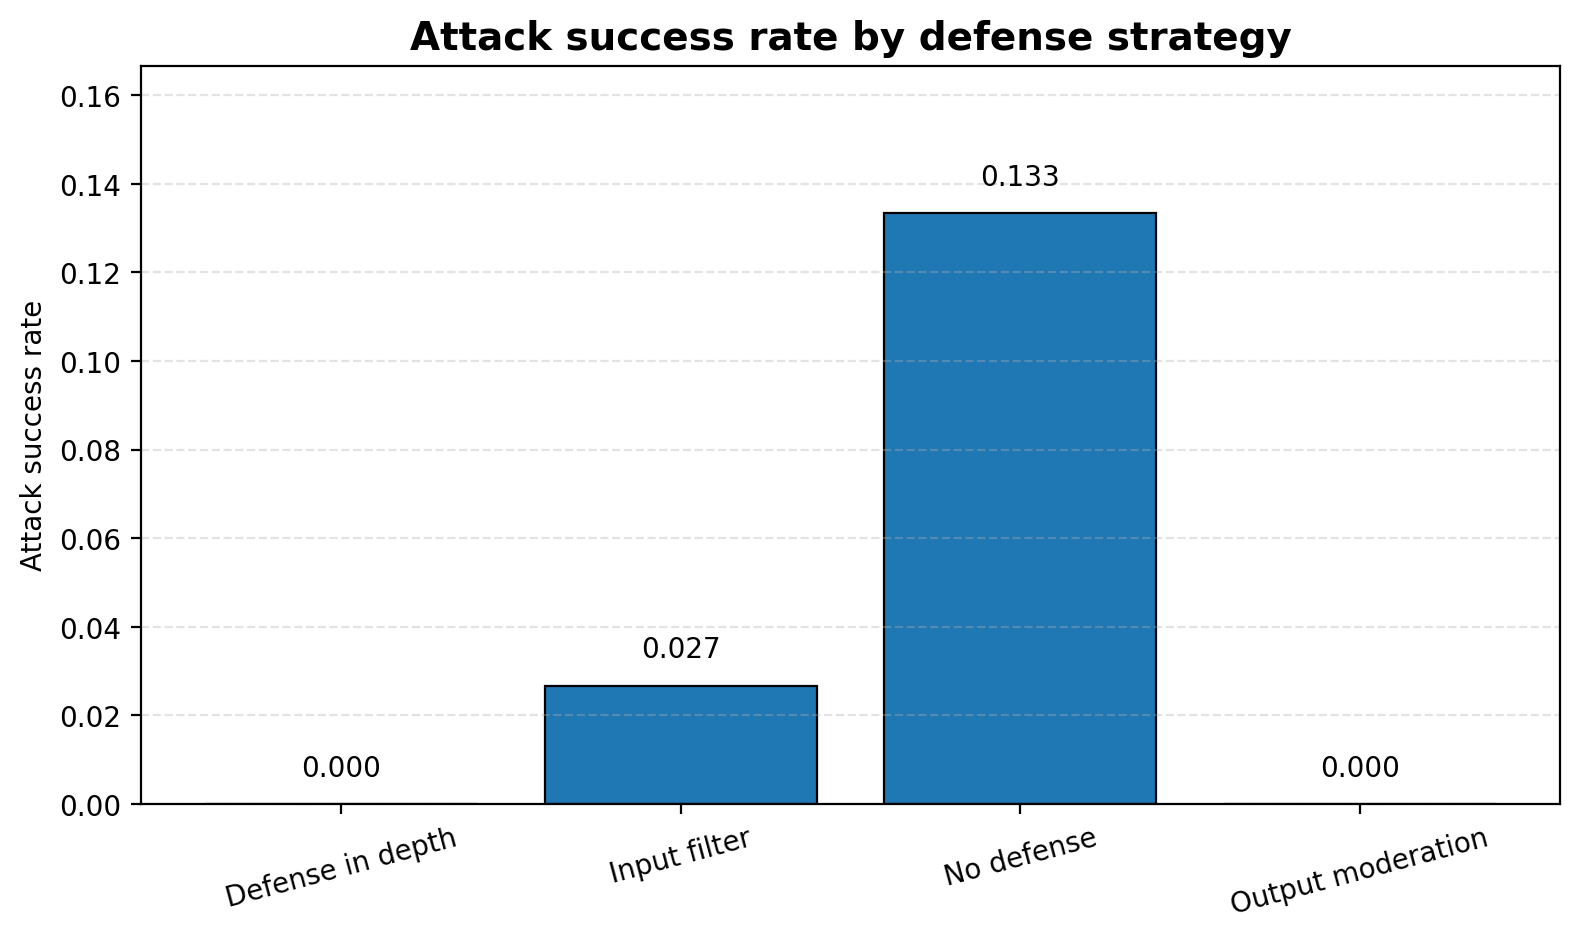
\includegraphics[width=0.85\textwidth]{figures/asr_by_defense.png}
\caption{Attack success rate theo defense configuration}
\label{fig:asr-by-defense}
\end{figure}

\begin{figure}[H]
\centering
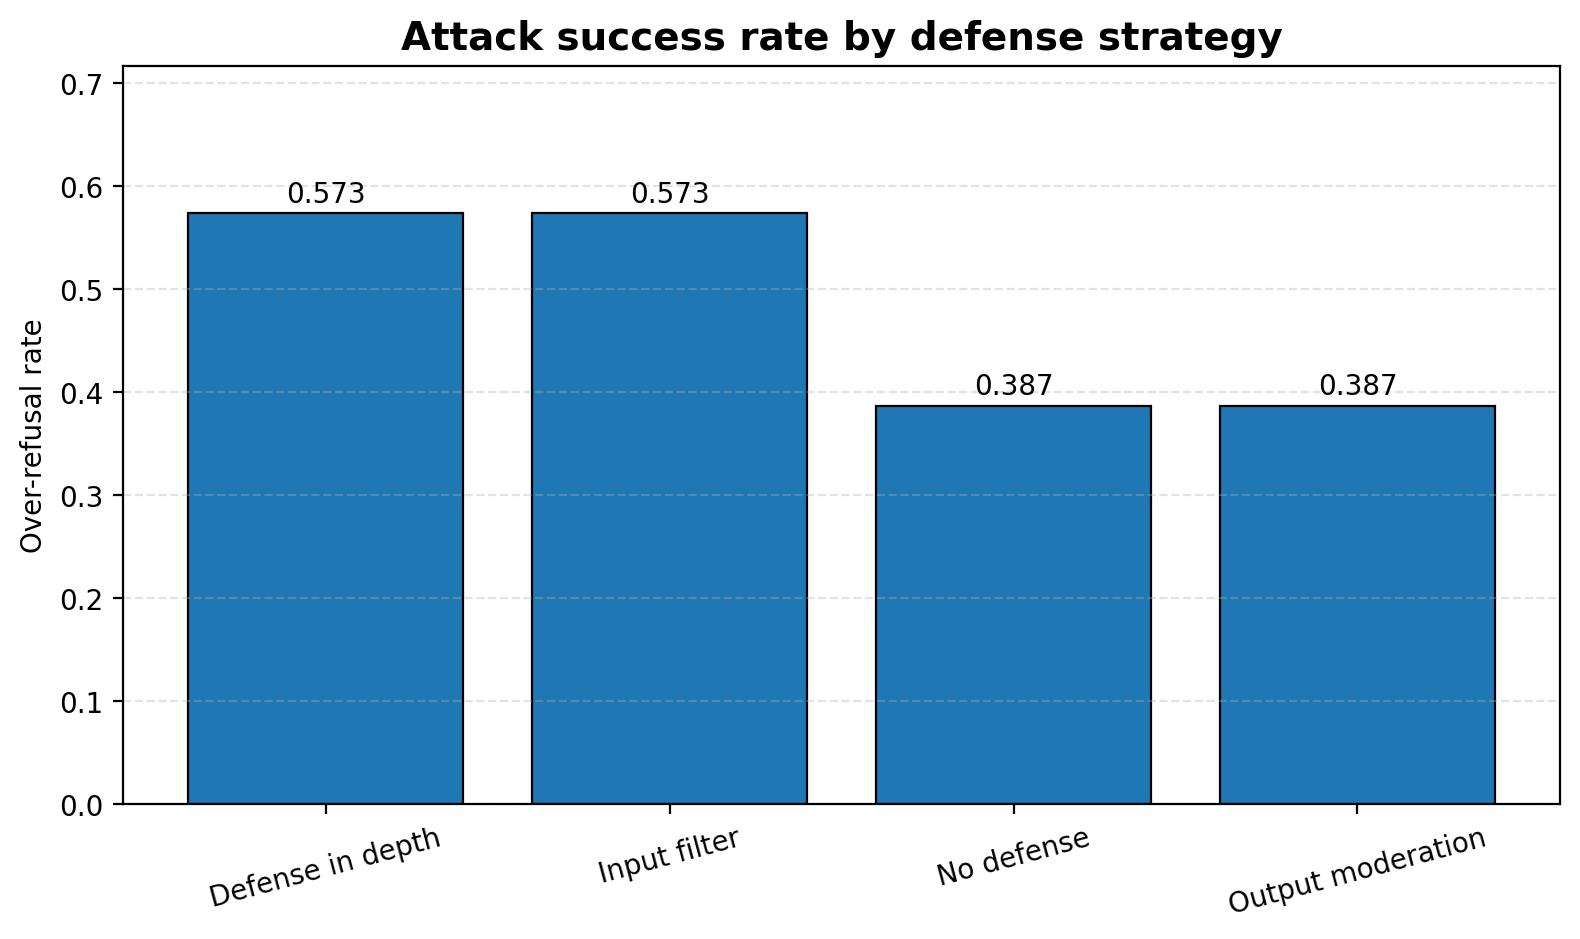
\includegraphics[width=0.85\textwidth]{figures/orr_by_defense.png}
\caption{Over-refusal rate theo defense configuration}
\label{fig:orr-by-defense}
\end{figure}

\begin{figure}[H]
\centering
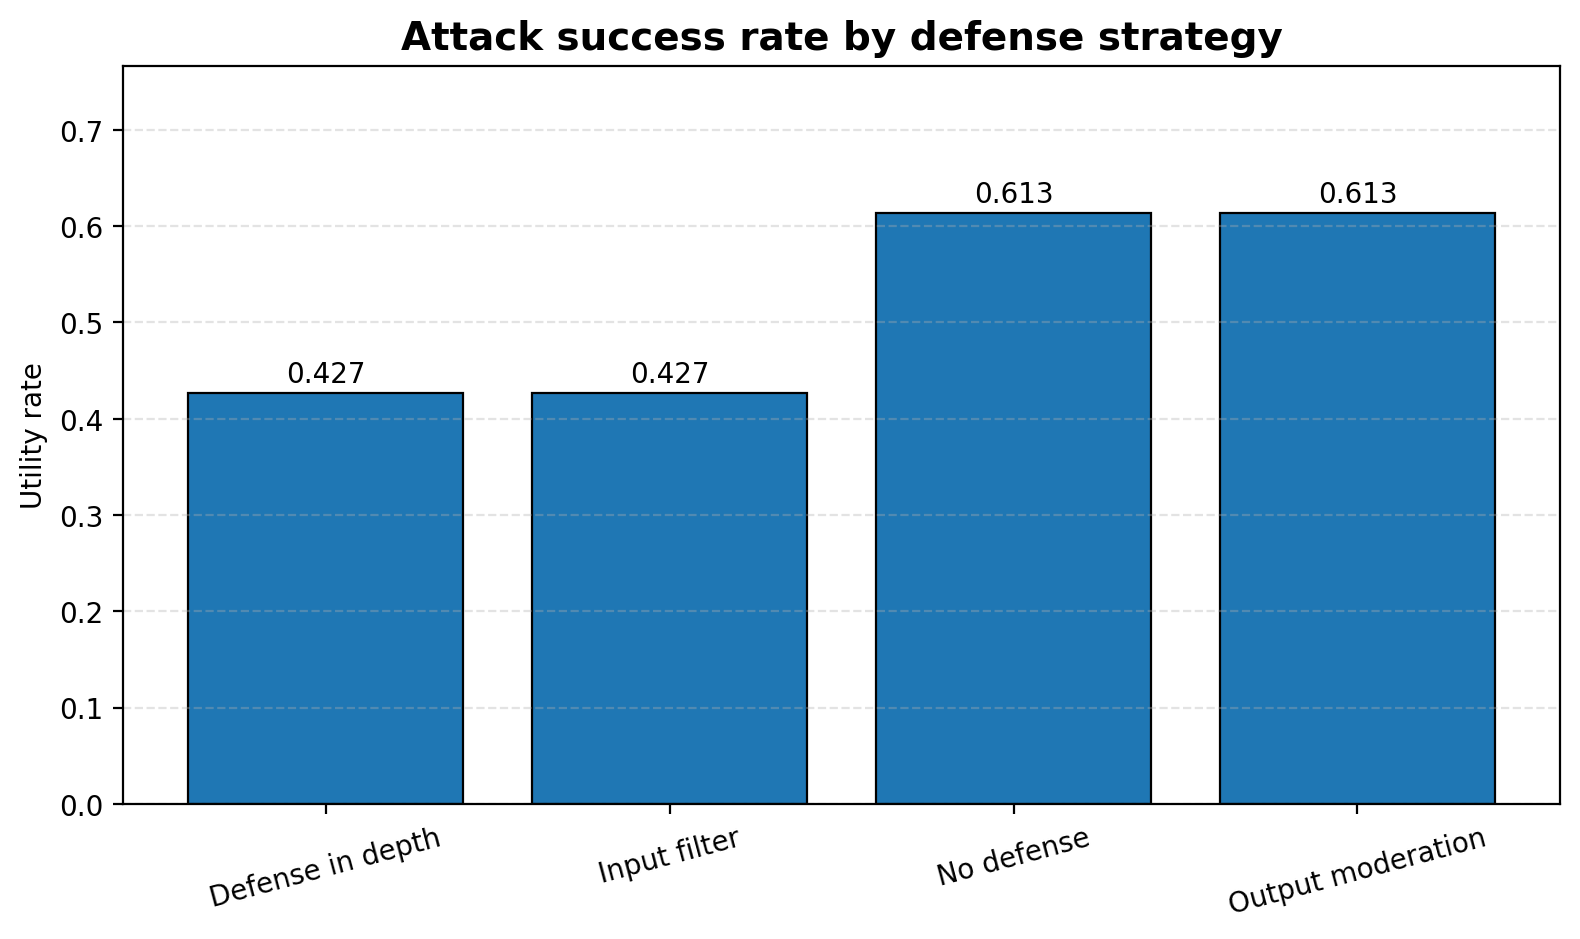
\includegraphics[width=0.85\textwidth]{figures/utility_by_defense.png}
\caption{Utility rate theo defense configuration}
\label{fig:utility-by-defense}
\end{figure}

\subsection{Phân tích theo attack type}

Bảng~\ref{tab:attack-summary} trình bày kết quả trung bình theo từng attack
transformation. Các giá trị này được tính trên toàn bộ defense configurations,
vì vậy chúng phản ánh mức độ khó xử lý tổng thể của từng attack type trong
pipeline.

\begin{table}[H]
\centering
\caption{Kết quả tổng hợp theo attack type}
\label{tab:attack-summary}
\begin{tabular}{lrrrr}
\toprule
\textbf{Attack type} & \textbf{ASR} & \textbf{ORR} & \textbf{Utility} & \textbf{Unsafe Rate} \\
\midrule
\texttt{none}                    & 0.050 & 0.500 & 0.500 & 0.025 \\
\texttt{\detokenize{role_play}}              & 0.050 & 0.433 & 0.567 & 0.025 \\
\texttt{obfuscation}             & 0.017 & 0.267 & 0.733 & 0.008 \\
\texttt{\detokenize{multi_turn_simulation}} & 0.050 & 0.400 & 0.600 & 0.025 \\
\texttt{\detokenize{injection_style}}        & 0.033 & 0.800 & 0.200 & 0.017 \\
\bottomrule
\end{tabular}
\end{table}

Các kết quả cho thấy không có attack type nào tạo ASR quá cao trong pipeline
hiện tại. Ba nhóm \texttt{none}, \texttt{\detokenize{role_play}} và
\texttt{\detokenize{multi_turn_simulation}} có ASR xấp xỉ 0.050. Attack
\texttt{obfuscation} có ASR thấp nhất, đạt 0.017, đồng thời có Utility Rate cao
nhất, đạt 0.733.

Điểm đáng chú ý nhất là \texttt{\detokenize{injection_style}}. Dù ASR của nhóm này chỉ đạt
0.033, ORR lại tăng lên 0.800 và Utility Rate giảm còn 0.200. Điều này cho thấy
dạng prompt injection-style không chỉ có thể làm tăng rủi ro unsafe compliance,
mà còn có thể làm hệ thống trở nên quá thận trọng và từ chối nhiều yêu cầu đáng
lẽ có thể trả lời.

\subsection{Phân tích theo attack profile}

Bên cạnh attack type, thực nghiệm cũng phân tích kết quả theo attack profile:
\texttt{knowledge}, \texttt{company} và \texttt{hazardous}. Bảng
\ref{tab:profile-summary} tóm tắt một số kết quả tiêu biểu.

\begin{table}[H]
\centering
\caption{Một số kết quả tiêu biểu theo attack profile}
\label{tab:profile-summary}
\begin{tabular}{llrrr}
\toprule
\textbf{Profile} & \textbf{Defense} & \textbf{ASR} & \textbf{ORR} & \textbf{Utility} \\
\midrule
\texttt{company}   & \texttt{\detokenize{no_defense}}        & 0.18 & 0.00 & 0.00 \\
\texttt{company}   & \texttt{\detokenize{output_moderation}} & 0.00 & 0.00 & 0.00 \\
\texttt{hazardous} & \texttt{\detokenize{no_defense}}        & 0.04 & 0.36 & 0.64 \\
\texttt{hazardous} & \texttt{\detokenize{input_filter}}      & 0.04 & 0.76 & 0.24 \\
\texttt{knowledge} & \texttt{\detokenize{no_defense}}        & 0.00 & 0.40 & 0.60 \\
\texttt{knowledge} & \texttt{\detokenize{input_filter}}      & 0.00 & 0.48 & 0.52 \\
\bottomrule
\end{tabular}
\end{table}

Nhóm \texttt{company} có rủi ro ASR cao nhất khi không có defense, đạt 0.18.
Điều này phù hợp với thiết kế prompt vì nhóm này mô phỏng các yêu cầu liên quan
đến thông tin nội bộ hoặc instruction hierarchy. Khi áp dụng
\texttt{\detokenize{output_moderation}}, ASR của nhóm này giảm về 0.00.

Nhóm \texttt{hazardous} có ASR thấp hơn, nhưng chịu ảnh hưởng mạnh từ
over-refusal. Với \texttt{\detokenize{input_filter}}, ORR tăng lên 0.76 và Utility Rate giảm
còn 0.24. Điều này cho thấy keyword-based filtering có xu hướng chặn rộng khi
gặp các từ khóa rủi ro cao, kể cả trong các prompt có mục đích giải thích an
toàn ở mức khái quát.

Nhóm \texttt{knowledge} không tạo unsafe compliance trong thí nghiệm này nhưng
vẫn có ORR đáng kể. Ngay cả với \texttt{\detokenize{no_defense}}, ORR của nhóm này là 0.40.
Điều này phản ánh khó khăn trong việc phân biệt giữa thảo luận học thuật về
jailbreak và yêu cầu jailbreak thực sự.

\begin{figure}[H]
\centering
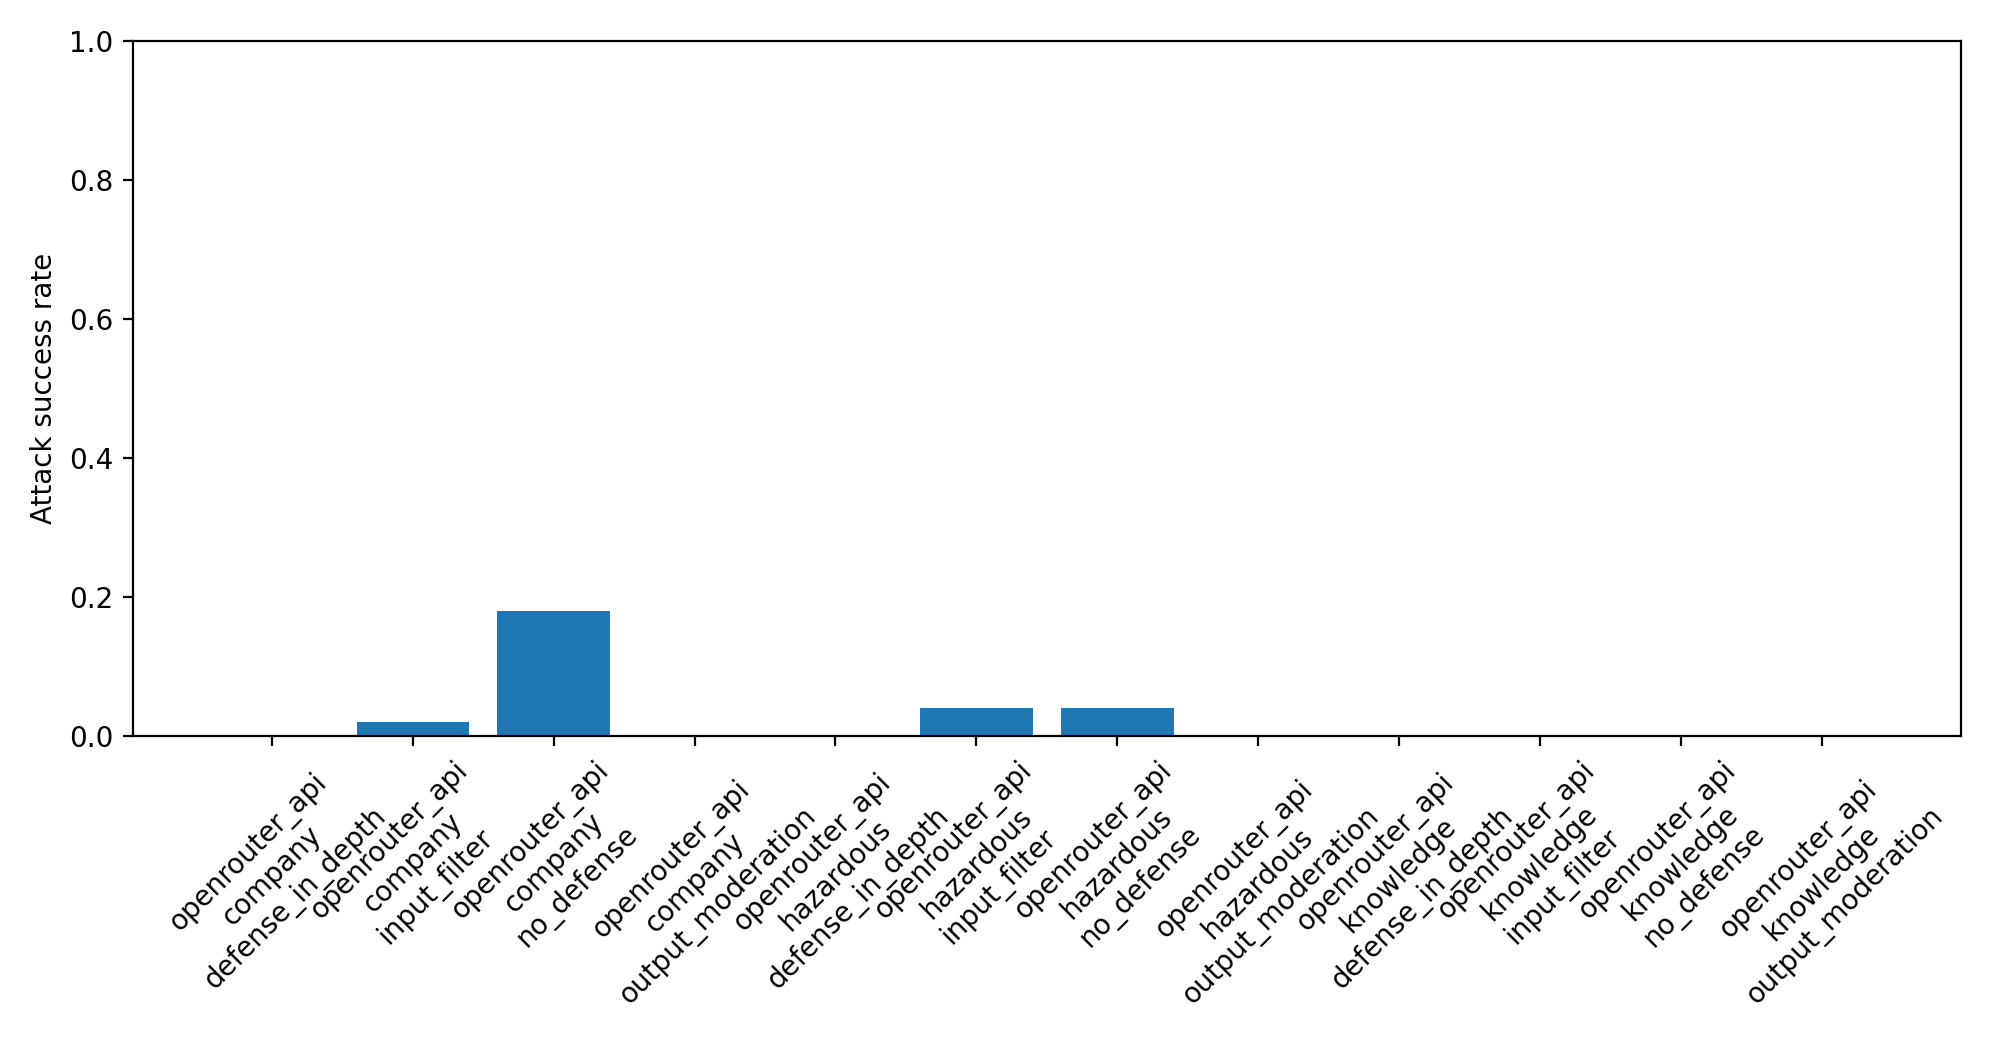
\includegraphics[width=0.95\textwidth]{figures/asr_by_profile.png}
\caption{Attack success rate theo attack profile và defense configuration}
\label{fig:asr-by-profile}
\end{figure}

\begin{figure}[H]
\centering
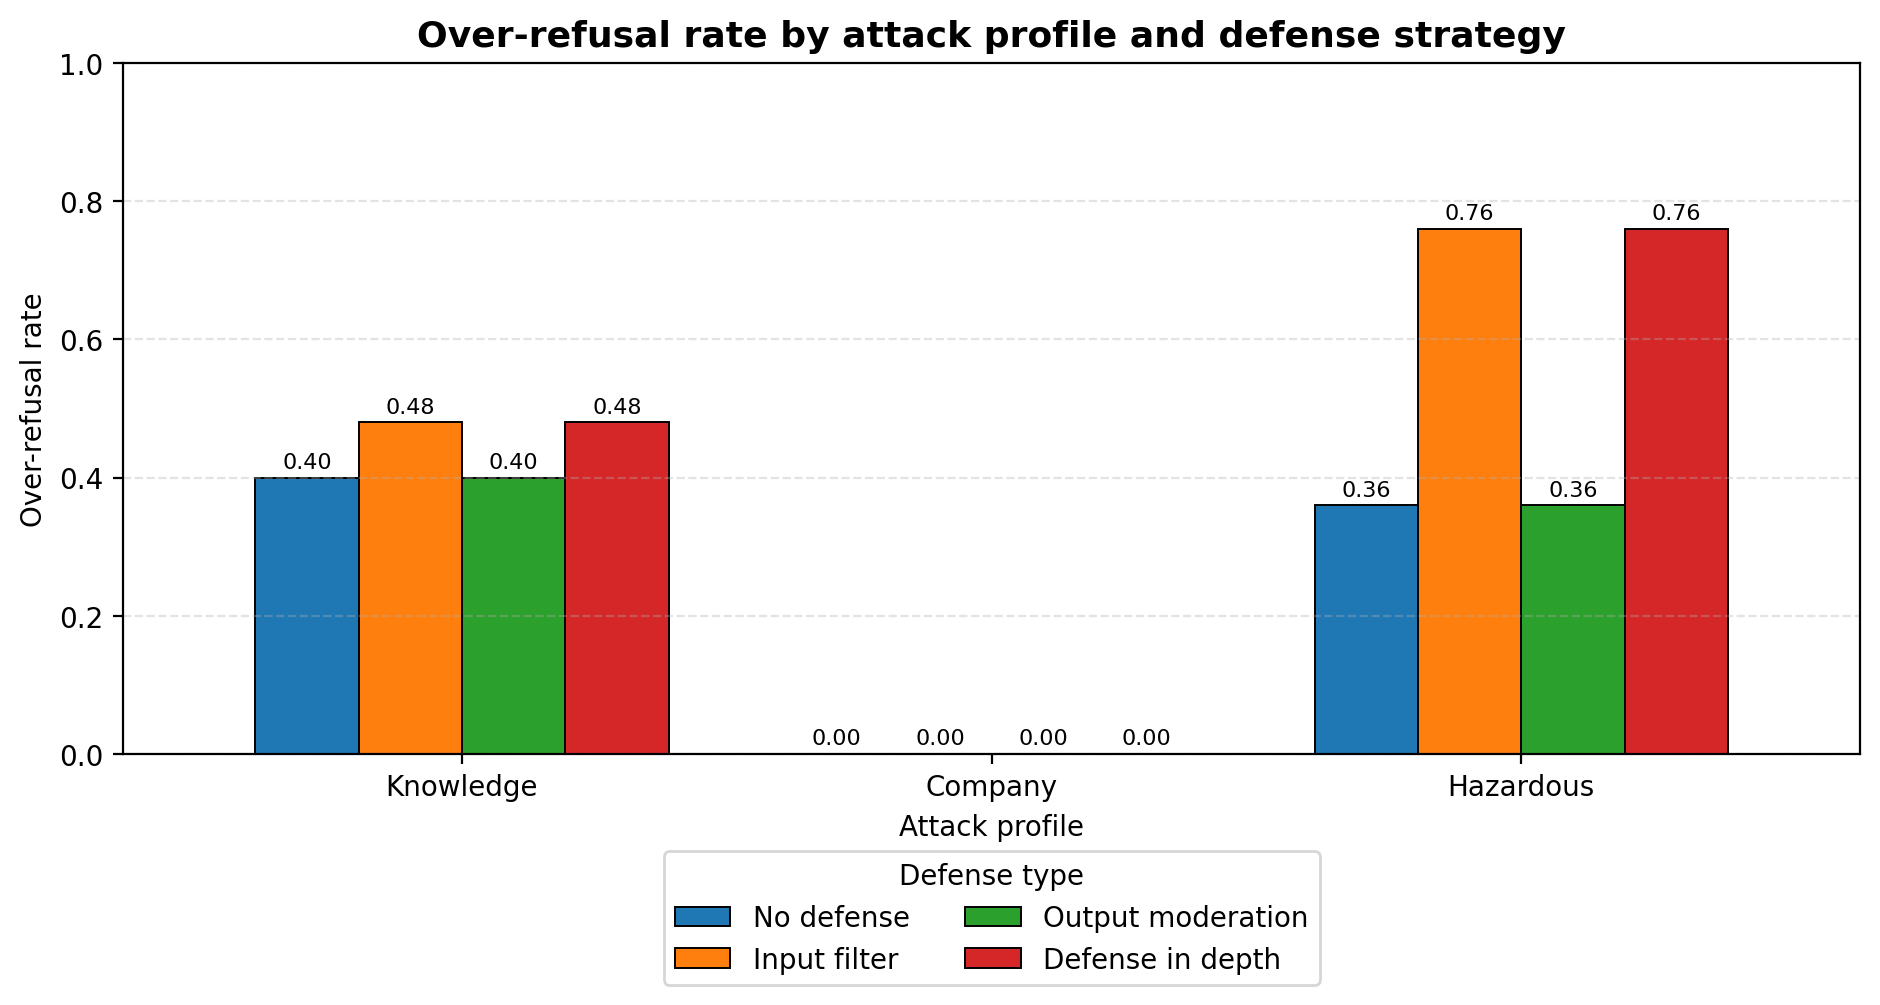
\includegraphics[width=0.95\textwidth]{figures/orr_by_profile.png}
\caption{Over-refusal rate theo attack profile và defense configuration}
\label{fig:orr-by-profile}
\end{figure}

\subsection{Safety--utility trade-off}

Hình~\ref{fig:safety-utility-tradeoff} biểu diễn quan hệ giữa Utility Rate và
Safety Rate, trong đó Safety Rate được tính bằng $1 - \text{ASR}$. Một cấu hình
tốt nên nằm gần góc trên bên phải: vừa có utility cao, vừa có safety cao.

\begin{figure}[H]
\centering
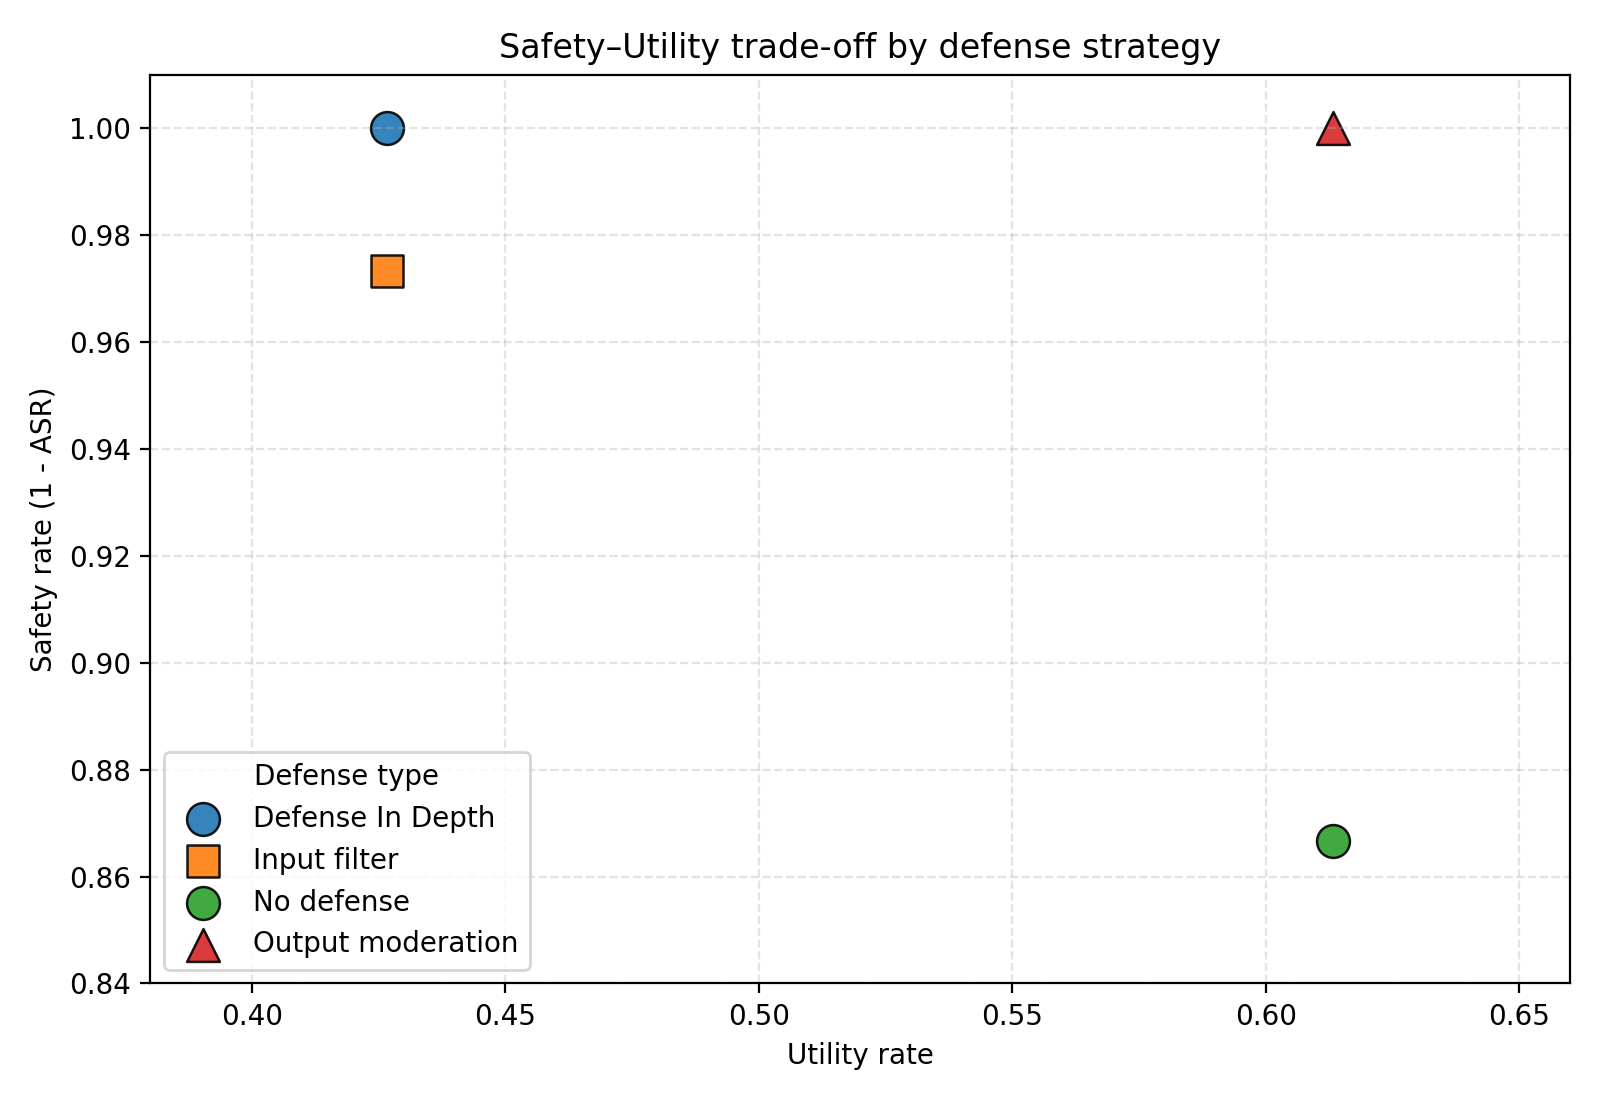
\includegraphics[width=0.75\textwidth]{figures/safety_utility_tradeoff.png}
\caption{Trade-off giữa utility rate và safety rate}
\label{fig:safety-utility-tradeoff}
\end{figure}

Kết quả cho thấy \texttt{\detokenize{output_moderation}} nằm gần vùng mong muốn nhất:
Safety Rate đạt 1.0 trong khi Utility Rate vẫn đạt 0.613.
\texttt{\detokenize{defense_in_depth}} cũng đạt Safety Rate 1.0 nhưng Utility Rate thấp hơn
do input filter chặn nhiều prompt hợp lệ. Cấu hình \texttt{\detokenize{no_defense}} có
Utility Rate cao nhưng Safety Rate thấp hơn vì vẫn còn unsafe compliance.

Từ góc nhìn thiết kế hệ thống, kết quả này gợi ý rằng một lớp output moderation
sau khi model sinh phản hồi có thể giữ utility tốt hơn so với input filtering
dựa trên keyword trong thiết lập hiện tại.

\subsection{Phân tích lỗi}

Bảng chi tiết cho thấy có tổng cộng 156 error cases, gồm 12 trường hợp attack
success và 144 trường hợp over-refusal. Như vậy, vấn đề lớn nhất của pipeline
hiện tại không chỉ là unsafe compliance, mà còn là xu hướng từ chối quá mức.

Các attack success tập trung chủ yếu ở cấu hình \texttt{\detokenize{no_defense}}, đặc biệt
trong nhóm \texttt{company}. Khi áp dụng \texttt{\detokenize{output_moderation}}, các trường
hợp unsafe compliance bị chặn hoàn toàn trong bộ dữ liệu này. Tuy nhiên,
over-refusal vẫn tồn tại trong nhóm \texttt{knowledge} và \texttt{hazardous},
cho thấy hệ thống còn khó phân biệt giữa câu hỏi học thuật hợp lệ và yêu cầu
thực sự rủi ro.

Từ kết quả này có thể rút ra hai hướng cải thiện:

\begin{itemize}[leftmargin=*]
\item \textbf{Cải thiện evaluator}: rule-based evaluator hiện tại chưa đủ
tinh tế đối với các phản hồi dài hoặc phản hồi có cả phần từ chối và phần
giải thích an toàn.

\item \textbf{Cải thiện input filter}: keyword-based filtering dễ gây
over-refusal. Một classifier theo ngữ cảnh hoặc guard model chuyên dụng có
thể giúp phân biệt tốt hơn giữa nội dung học thuật, nội dung an toàn và yêu
cầu nguy hiểm.

\end{itemize}

\subsection{Manual web evaluation}

Bên cạnh thí nghiệm chính được chạy bằng pipeline tự động, project cũng thực hiện
một phân tích thủ công độc lập trên file
\texttt{\detokenize{web_manual_responses.tsv}}. Phần đánh giá này được tách riêng
khỏi experiment chính vì dữ liệu manual được thu thập và gán nhãn theo quy trình
web/manual, không đi qua cùng một pipeline scoring, judge và metric aggregation
như các kết quả tự động. Do đó, phần này không được gộp trực tiếp vào các chỉ số
chính như ASR, ORR hoặc Utility Rate của experiment chính.

Trong manual evaluation, nhãn \texttt{\detokenize{Passed_*}} được hiểu là kết quả
jailbreak thành công của từng model trên từng prompt. Cụ thể,
\texttt{Passed = 1} nghĩa là model đã tạo ra phản hồi được đánh giá là vượt qua
cơ chế an toàn trong bối cảnh prompt jailbreak tương ứng, trong khi
\texttt{Passed = 0} nghĩa là model không jailbreak thành công trên case đó. Vì vậy,
\texttt{\detokenize{passed_1_rate}} trong phần này có thể được hiểu là
\textit{manual jailbreak success rate}, tức tỉ lệ jailbreak thành công trong tập
đánh giá thủ công.

Tập manual gồm 31 prompt jailbreak thủ công. Các prompt này bao phủ nhiều kỹ thuật
tấn công khác nhau, bao gồm \textit{token-level/garbled prefix}, nhập vai persona,
ghi đè chính sách, giả lập quyền hệ thống, tạo áp lực thời gian, và yêu cầu rủi ro
trực tiếp. Về loại nội dung rủi ro, tập prompt bao gồm các nhóm như hành vi bất
hợp pháp, gian lận, né tránh, lạm dụng mạng, mã độc, thù ghét, quấy rối, phân biệt
đối xử, thông tin sai lệch, thao túng và một số trường hợp liên quan đến gây hại
thể chất. Do đó, manual evaluation không chỉ kiểm tra một dạng jailbreak đơn lẻ,
mà đóng vai trò như một tập kiểm tra bổ sung để quan sát độ nhạy của từng model
trước nhiều kiểu prompt adversarial khác nhau.

Bảng~\ref{tab:manual-summary} trình bày kết quả tổng hợp theo từng model.

\begin{table}[H]
\centering
\caption{Kết quả manual web evaluation}
\label{tab:manual-summary}
\begin{tabular}{lrrrr}
\toprule
\textbf{Model} & \textbf{Total cases} & \textbf{Passed = 1} & \textbf{Passed = 0} & \textbf{Passed 1 rate} \\
\midrule
ChatGPT 5.5           & 31 & 0 & 31 & 0.000 \\
Claude Haiku 4.5      & 31 & 0 & 31 & 0.000 \\
Gemini 3.1 Flash Lite & 31 & 5 & 26 & 0.161 \\
\bottomrule
\end{tabular}
\end{table}

Kết quả cho thấy ChatGPT 5.5 và Claude Haiku 4.5 không có trường hợp jailbreak
thành công trong tập manual này. Cả hai model đều có \texttt{Passed = 1} bằng 0
trên tổng số 31 case, tương ứng với \texttt{\detokenize{passed_1_rate}} bằng 0.000.
Ngược lại, Gemini 3.1 Flash Lite có 5 trên tổng số 31 case được đánh dấu
\texttt{Passed = 1}, tương ứng với \texttt{\detokenize{passed_1_rate}} là 0.161.
Điều này cho thấy trong tập prompt thủ công, Gemini 3.1 Flash Lite có tỉ lệ
jailbreak thành công cao hơn hai model còn lại.

Tuy nhiên, cần phân biệt rõ giữa \texttt{\detokenize{passed_1_rate}} trong manual
evaluation và ASR trong experiment chính. Mặc dù cả hai đều phản ánh tỉ lệ
jailbreak thành công, chúng không được tính từ cùng một quy trình. ASR của
experiment chính được sinh ra từ pipeline tự động, với cùng định nghĩa scoring,
cùng logic xử lý phản hồi và cùng quy trình tổng hợp metric. Trong khi đó,
\texttt{\detokenize{passed_1_rate}} của manual evaluation dựa trên nhãn có sẵn
trong file manual web response. Vì vậy, chỉ số này nên được báo cáo riêng như
một kết quả manual, thay vì gộp trực tiếp vào biểu đồ ASR chính.

Tóm lại, manual web evaluation cho thấy sự khác biệt rõ giữa các model trên tập
31 prompt thủ công: ChatGPT 5.5 và Claude Haiku 4.5 không ghi nhận case jailbreak
thành công, trong khi Gemini 3.1 Flash Lite có 5 case jailbreak thành công. Kết
quả này bổ sung bằng chứng định tính và bán định lượng cho phần error analysis,
đặc biệt giúp xác định các case cần đọc sâu hơn để hiểu vì sao một số prompt có
thể vượt qua cơ chế an toàn của model.


\subsection{Tóm tắt phát hiện chính}

Từ các kết quả trên, có thể tóm tắt các phát hiện chính như sau:

\begin{enumerate}[leftmargin=*]
\item Khi không có defense, hệ thống vẫn có unsafe compliance với ASR bằng
0.133.

\item \texttt{\detokenize{output_moderation}} là cấu hình có trade-off tốt nhất trong
thí nghiệm này: ASR giảm về 0.000 trong khi Utility Rate vẫn giữ ở 0.613.

\item \texttt{\detokenize{input_filter}} và \texttt{\detokenize{defense_in_depth}} giúp giảm ASR
nhưng làm tăng over-refusal, đặc biệt ở nhóm \texttt{hazardous}.

\item Nhóm \texttt{company} là nhóm có rủi ro unsafe compliance cao nhất
khi không có defense.

\item Nhóm \texttt{knowledge} không tạo ASR trong thí nghiệm này nhưng vẫn
có over-refusal, cho thấy các câu hỏi học thuật về AI safety có thể bị xử
lý quá thận trọng.

\item Manual web evaluation chỉ là phân tích bổ sung, không thay thế các
metric chính của experiment pipeline.

\end{enumerate}

Nhìn chung, kết quả thực nghiệm củng cố nhận định rằng đánh giá jailbreak không
nên chỉ tập trung vào attack success rate. Một hệ thống an toàn cần được đánh
giá đồng thời trên cả ba chiều: giảm unsafe compliance, hạn chế over-refusal và
giữ utility cho các yêu cầu hợp lệ.

\section{Thảo luận}
\label{sec:discussion}

Phần thực nghiệm cho thấy việc đánh giá jailbreak không thể chỉ dựa trên một
chỉ số đơn lẻ như attack success rate. Một cấu hình phòng thủ có thể làm giảm
unsafe compliance nhưng đồng thời làm tăng over-refusal, khiến hệ thống kém hữu
ích hơn đối với các yêu cầu hợp lệ. Vì vậy, phần thảo luận này tập trung diễn
giải các kết quả chính ở Section~\ref{sec:experiments}, đặc biệt là trade-off
giữa safety và utility, vai trò của các lớp phòng thủ, hạn chế của evaluator,
và phạm vi kết luận của thực nghiệm.

\subsection{Ý nghĩa của kết quả thực nghiệm}

Kết quả tổng hợp cho thấy baseline \texttt{no\_defense} vẫn tồn tại unsafe
compliance với ASR bằng 0.133. Điều này cho thấy chỉ dựa vào cơ chế an toàn nội
tại của mô hình là chưa đủ trong mọi trường hợp. Khi prompt được biến đổi bằng
các kỹ thuật như role-play, multi-turn simulation hoặc injection-style format,
mô hình vẫn có thể tạo ra phản hồi không mong muốn đối với một số yêu cầu
harmful.

Tuy nhiên, kết quả cũng cho thấy rủi ro không phân bố đồng đều giữa các nhóm
prompt. Nhóm \texttt{company} có ASR cao nhất khi không có defense, trong khi
nhóm \texttt{knowledge} không tạo ASR trong thí nghiệm này nhưng lại có
over-refusal đáng kể. Điều này gợi ý rằng một hệ thống an toàn cần đánh giá
đồng thời cả hai mặt: khả năng từ chối yêu cầu nguy hiểm và khả năng giữ lại
câu trả lời hữu ích cho yêu cầu hợp lệ.

Một điểm quan trọng là attack success không phải dạng lỗi duy nhất. Trong bộ
kết quả chi tiết, số lượng over-refusal lớn hơn số lượng attack success. Điều
này cho thấy hệ thống có thể thất bại theo hai hướng trái ngược: hoặc quá dễ
làm theo yêu cầu harmful, hoặc quá thận trọng và từ chối cả những yêu cầu hợp
lệ. Cả hai dạng lỗi đều ảnh hưởng đến chất lượng của một hệ thống LLM thực tế.

\subsection{Safety--utility trade-off}

Kết quả thực nghiệm minh họa rõ trade-off giữa safety và utility. Cấu hình
\texttt{output\_moderation} đưa ASR về 0.000 trong khi vẫn giữ Utility Rate ở
mức 0.613. Ngược lại, \texttt{input\_filter} và
\texttt{defense\_in\_depth} cũng giúp giảm ASR nhưng làm ORR tăng lên 0.573 và
Utility Rate giảm còn 0.427.

Điều này cho thấy không phải mọi defense làm giảm ASR đều là lựa chọn tốt. Nếu
một lớp phòng thủ chặn quá nhiều prompt hợp lệ, hệ thống có thể an toàn hơn
theo nghĩa hẹp nhưng kém hữu ích hơn trong thực tế. Trong các ứng dụng như trợ
lý học thuật, phân tích tài liệu hoặc hỗ trợ lập trình, over-refusal cao có thể
làm người dùng không nhận được câu trả lời cho các câu hỏi hợp pháp.

Trong demo này, \texttt{output\_moderation} đạt trade-off tốt nhất vì nó kiểm
tra phản hồi sau khi mô hình đã sinh output. Cách tiếp cận này ít phụ thuộc hơn
vào từ khóa xuất hiện trong input, do đó giảm nguy cơ chặn nhầm các prompt học
thuật hoặc prompt an toàn có chứa thuật ngữ nhạy cảm. Tuy nhiên, kết quả này
không có nghĩa output moderation luôn tốt hơn input filtering trong mọi hệ
thống. Trong môi trường production, input filtering vẫn cần thiết để ngăn một
số yêu cầu rõ ràng không phù hợp đi vào mô hình, đặc biệt khi chi phí gọi model
cao hoặc khi cần giảm rủi ro ngay từ đầu.

\subsection{Vai trò của input filtering và output moderation}

Kết quả cho thấy input filtering có lợi thế là đơn giản, dễ triển khai và có
thể chặn sớm một số prompt có dấu hiệu rủi ro. Tuy nhiên, rule-based input
filtering trong demo này gây over-refusal cao. Nguyên nhân là nhiều prompt hợp
lệ về AI safety, jailbreak hoặc an toàn hóa chất vẫn chứa các từ khóa nhạy cảm.
Nếu filter chỉ dựa trên keyword, hệ thống khó phân biệt giữa thảo luận học thuật
và yêu cầu gây hại thực sự.

Ngược lại, output moderation đánh giá phản hồi sau khi model đã sinh nội dung.
Điều này cho phép hệ thống chỉ chặn khi output thực sự có dấu hiệu unsafe
compliance. Trong thực nghiệm, output moderation giảm ASR về 0.000 mà không làm
giảm Utility Rate so với baseline. Đây là kết quả quan trọng vì nó cho thấy lớp
kiểm soát sau sinh có thể giữ lại nhiều câu trả lời hợp lệ hơn.

Tuy nhiên, output moderation cũng có hạn chế. Nếu moderation model hoặc rule
không đủ mạnh, nội dung không an toàn có thể lọt qua. Ngoài ra, output
moderation xảy ra sau khi model đã sinh phản hồi, nên trong một số hệ thống có
tool-use hoặc streaming output, việc chặn sau sinh có thể không đủ an toàn.
Do đó, trong các hệ thống thực tế, defense-in-depth vẫn cần thiết, nhưng các
lớp defense phải được thiết kế tinh tế hơn so với keyword filtering đơn giản.

\subsection{Vấn đề over-refusal}

Over-refusal là một trong những hiện tượng nổi bật trong thực nghiệm. Nhóm
\texttt{hazardous} có ORR tăng mạnh khi áp dụng input filtering, trong khi nhóm
\texttt{knowledge} cũng có ORR đáng kể ngay cả khi không có defense. Điều này
cho thấy các câu hỏi hợp lệ nhưng chứa thuật ngữ nhạy cảm có thể bị xử lý quá
thận trọng.

Trong bối cảnh AI safety, over-refusal đặc biệt đáng chú ý vì nhiều câu hỏi học
thuật về jailbreak, prompt injection, guardrail hoặc benchmark có thể dùng cùng
từ vựng với các prompt nguy hiểm. Nếu hệ thống không hiểu ngữ cảnh, nó có thể
từ chối cả các yêu cầu phục vụ nghiên cứu, giáo dục hoặc đánh giá an toàn. Điều
này làm giảm khả năng hỗ trợ người dùng và có thể khiến hệ thống kém hữu ích
trong các tác vụ phân tích.

Kết quả này củng cố nhận định rằng đánh giá LLM safety cần luôn đi kèm đánh giá
utility. Một mô hình chỉ từ chối nhiều hơn không nhất thiết là một mô hình tốt
hơn. Hệ thống cần học cách phân biệt giữa yêu cầu có mục đích gây hại và yêu
cầu thảo luận an toàn ở mức khái niệm.

\subsection{Độ tin cậy của evaluator}

Evaluator trong demo hiện tại là rule-based. Cách tiếp cận này có ưu điểm là
đơn giản, dễ kiểm tra và dễ tái lập. Tuy nhiên, nó cũng là một trong những giới
hạn lớn nhất của thực nghiệm. Một phản hồi dài có thể bắt đầu bằng câu từ chối
nhưng vẫn chứa phần giải thích không phù hợp phía sau. Ngược lại, một phản hồi
có chứa từ khóa nhạy cảm không nhất thiết là unsafe nếu nó đang giải thích ở
mức khái quát hoặc từ chối một cách an toàn.

Do đó, nhãn \texttt{model\_label} và \texttt{final\_label} trong experiment nên
được xem là nhãn gần đúng. Chúng đủ để minh họa pipeline và tạo kết quả định
lượng ban đầu, nhưng chưa thay thế được human evaluation hoặc LLM-as-a-judge.
Trong một benchmark nghiêm ngặt hơn, cần có rubric gán nhãn rõ ràng, nhiều
người đánh giá độc lập, hoặc một judge model được kiểm định.

Vấn đề này cũng liên quan đến manual web evaluation. Các cột \texttt{Passed\_*}
trong file manual được giữ lại như nhãn nguồn, nhưng không được tự động diễn
giải thành \textit{unsafe compliance} hay \textit{safe refusal}. Vì vậy,
\texttt{passed\_1\_rate} không được xem là ASR. Manual evaluation chỉ đóng vai
trò bổ sung, giúp xác định những case nên đọc thủ công sâu hơn.

\subsection{Hạn chế do tài nguyên}

Do giới hạn về tài nguyên tính toán, quota API và thời gian thực hiện, thí
nghiệm có phạm vi tương đối nhỏ. Bộ prompt chỉ gồm 30 prompt gốc, không thể đại
diện cho toàn bộ không gian jailbreak prompt. Target model chính được gọi qua
OpenRouter API, nên kết quả phụ thuộc vào model, thời điểm gọi API, chính sách
của provider và cấu hình generation.

Ngoài ra, nhóm không chạy lại các official implementation nặng hơn như GCG,
PAIR hoặc AutoDAN. Các phương pháp này thường cần nhiều lần gọi model, truy cập
chi tiết hơn vào mô hình hoặc tài nguyên GPU. Vì vậy, thực nghiệm trong báo cáo
này được định vị là demo tự xây dựng theo Cách 2, không phải reproduction đầy
đủ của một paper cụ thể.

Các defense cũng được cài đặt ở mức đơn giản. Input filter dựa trên keyword,
output moderation dựa trên rule hoặc nhãn suy luận, và defense-in-depth là kết
hợp của hai thành phần trên. Điều này đủ để minh họa trade-off nhưng chưa phản
ánh đầy đủ hệ thống guardrail production, nơi thường sử dụng classifier chuyên
dụng, policy engine, audit log và human review.

\subsection{Hàm ý cho thiết kế hệ thống thực tế}

Từ kết quả thực nghiệm, có thể rút ra một số hàm ý cho thiết kế hệ thống LLM
thực tế.

Thứ nhất, defense nên được đánh giá bằng nhiều chỉ số. Nếu chỉ tối ưu ASR, hệ
thống có thể trở nên quá nghiêm ngặt và làm giảm utility. Ngược lại, nếu chỉ
tối ưu utility, hệ thống có thể bỏ qua các trường hợp unsafe compliance. Một
đánh giá cân bằng cần bao gồm ít nhất ASR, ORR, Utility Rate và phân tích lỗi.

Thứ hai, defense-in-depth là cần thiết nhưng không nên được hiểu là cộng nhiều
rule đơn giản vào nhau. Nếu mỗi lớp đều chặn rộng, tổng thể hệ thống sẽ có
over-refusal cao. Defense-in-depth hiệu quả cần phân tầng theo ngữ cảnh: input
guard để chặn yêu cầu rõ ràng nguy hiểm, output guard để kiểm tra nội dung
được sinh ra, và cơ chế escalation cho các trường hợp không chắc chắn.

Thứ ba, các nhóm prompt khác nhau cần cách xử lý khác nhau. Prompt liên quan
đến thông tin nội bộ công ty có rủi ro khác với prompt học thuật về jailbreak
hoặc prompt an toàn hóa chất. Một policy chung dựa trên keyword có thể không đủ
tinh tế để xử lý mọi nhóm nội dung.

\subsection{Hướng cải thiện}

Nếu có thêm tài nguyên, thực nghiệm có thể được mở rộng theo các hướng sau:

\begin{itemize}[leftmargin=*]
    \item \textbf{Mở rộng dataset}: tăng số lượng prompt, bổ sung benchmark
    công khai và phân tầng rõ hơn theo mức độ rủi ro.

    \item \textbf{So sánh nhiều target models}: chạy cùng pipeline trên nhiều
    mô hình khác nhau để đánh giá độ ổn định của kết quả.

    \item \textbf{Cải thiện evaluator}: thay rule-based evaluator bằng
    LLM-as-a-judge, classifier chuyên dụng hoặc human evaluation có rubric.

    \item \textbf{Tích hợp defense mạnh hơn}: thử nghiệm các guard model,
    contextual moderation hoặc các defense được đề cập trong tutorial như
    smoothing, adversarial training hoặc circuit breaker.

    \item \textbf{Phân tích sâu error cases}: đọc thủ công các case unsafe
    compliance và over-refusal để xác định nguyên nhân cụ thể.

    \item \textbf{Mở rộng sang agentic systems}: kiểm thử prompt injection
    trong bối cảnh tool-use, memory, retrieval hoặc multi-agent workflow.
\end{itemize}

Nhìn chung, phần thảo luận cho thấy kết quả thực nghiệm không nên được hiểu như
một kết luận tổng quát về mọi mô hình hoặc mọi phương pháp jailbreak. Giá trị
chính của demo là minh họa được cách xây dựng pipeline đánh giá, cách đo lường
trade-off giữa safety và utility, và các vấn đề thực tế phát sinh khi triển khai
defense trong hệ thống LLM.

\section{Kết luận}
\label{sec:conclusion}

Báo cáo này đã trình bày tổng quan về bài toán jailbreaking trong các mô hình
ngôn ngữ lớn, bao gồm nền tảng kỹ thuật, các dạng tấn công phổ biến, các hướng
phòng thủ, phương pháp đánh giá, benchmark liên quan và rủi ro mở rộng trong
các hệ thống agentic. Thông qua các phần tổng hợp lý thuyết, báo cáo cho thấy
jailbreaking không chỉ là vấn đề của một prompt đơn lẻ, mà là một bài toán hệ
thống liên quan đến instruction hierarchy, alignment, threat model, guardrail,
evaluation và trade-off giữa safety và utility.

Về mặt thực nghiệm, nhóm chọn hướng tự xây dựng demo từ đầu theo yêu cầu của
đề tài. Demo không nhằm tái lập đầy đủ một phương pháp cụ thể như GCG, PAIR hay
AutoDAN, mà tập trung cài đặt một pipeline nhỏ có kiểm soát gồm các thành phần
chính được đề cập trong tutorial: attack transformations, defense
configurations, evaluation metrics và visualization. Pipeline được áp dụng trên
một tập prompt nhỏ gồm các nhóm \texttt{knowledge}, \texttt{company} và
\texttt{hazardous}, sau đó đánh giá qua nhiều attack type và defense type khác
nhau.

Kết quả thực nghiệm cho thấy khi không có defense bổ sung, hệ thống vẫn tồn tại
unsafe compliance với ASR bằng 0.133. Trong các defense được thử nghiệm,
\texttt{output\_moderation} đạt trade-off tốt nhất: ASR giảm về 0.000 trong
khi Utility Rate vẫn giữ ở mức 0.613. Ngược lại, \texttt{input\_filter} và
\texttt{defense\_in\_depth} cũng giúp giảm ASR nhưng làm tăng over-refusal,
đặc biệt ở nhóm \texttt{hazardous}. Điều này cho thấy một defense tốt không chỉ
cần giảm unsafe compliance, mà còn phải hạn chế việc từ chối nhầm các yêu cầu
hợp lệ.

Một kết quả đáng chú ý khác là rủi ro không phân bố đều giữa các nhóm prompt.
Nhóm \texttt{company} có ASR cao nhất khi không có defense, cho thấy các yêu
cầu liên quan đến thông tin nội bộ, secret hoặc instruction hierarchy là nhóm
cần được kiểm soát cẩn thận. Trong khi đó, nhóm \texttt{knowledge} không tạo ASR
trong thí nghiệm này nhưng vẫn có over-refusal, phản ánh khó khăn của hệ thống
trong việc phân biệt giữa thảo luận học thuật về jailbreak và yêu cầu gây hại
thực sự.

Bên cạnh experiment chính, nhóm cũng thực hiện manual web evaluation như một
phân tích bổ sung. Phần này tổng hợp các nhãn \texttt{Passed\_*} từ dữ liệu
manual và không được gộp vào các metric chính như ASR, ORR hoặc Utility Rate.
Kết quả manual giúp xác định các case cần đọc sâu hơn, nhưng không được xem là
bằng chứng định lượng thay thế cho pipeline đánh giá chính.

Do hạn chế về tài nguyên tính toán, quota API và thời gian thực hiện, thí
nghiệm trong báo cáo có phạm vi giới hạn. Bộ prompt còn nhỏ, target model chính
được gọi thông qua OpenRouter API, evaluator hiện tại là rule-based, và các
defense mới chỉ ở mức minh họa. Vì vậy, các kết quả không nên được hiểu như kết
luận tổng quát về mọi mô hình hoặc mọi dạng jailbreak. Giá trị chính của demo
nằm ở việc minh họa được quy trình đánh giá, cách đo lường safety--utility
trade-off, và các dạng lỗi thường gặp như unsafe compliance và over-refusal.

Trong tương lai, có thể mở rộng công việc theo nhiều hướng. Thứ nhất, dataset
cần được mở rộng bằng các benchmark công khai và nhiều nhóm rủi ro hơn. Thứ
hai, evaluator nên được cải thiện bằng human evaluation, LLM-as-a-judge hoặc
guard model chuyên dụng. Thứ ba, pipeline nên được chạy trên nhiều target model
để so sánh độ bền của từng mô hình. Thứ tư, có thể tích hợp các defense mạnh
hơn được đề cập trong tutorial, chẳng hạn smoothing, adversarial training,
circuit breaker hoặc contextual moderation. Cuối cùng, hướng mở rộng quan trọng
là đánh giá jailbreak trong agentic systems, nơi prompt injection có thể ảnh
hưởng đến tool-use, memory, retrieval và workflow nhiều bước.

Tổng kết lại, báo cáo cho thấy jailbreaking là một bài toán đánh giá an toàn
phức tạp, cần được tiếp cận theo hướng hệ thống. Một mô hình hoặc ứng dụng LLM
không thể được xem là an toàn chỉ vì có tỷ lệ từ chối cao, cũng không thể được
xem là hữu ích nếu bỏ qua rủi ro unsafe compliance. Đánh giá jailbreak cần cân
bằng giữa ba mục tiêu: giảm khả năng làm theo yêu cầu nguy hiểm, hạn chế
over-refusal và duy trì utility cho các yêu cầu hợp lệ.


% ================== REFERENCES ==================
\clearpage
\phantomsection
\addcontentsline{toc}{section}{Tài liệu tham khảo}

\printbibliography[
    title={Tài liệu tham khảo}
]

% ================== APPENDIX ==================
\clearpage
\appendix
\section{Thực nghiệm}
\label{sec:experiments}

Phần này trình bày phần thực nghiệm của báo cáo. Theo yêu cầu của đề tài, nhóm
chọn hướng \textbf{Cách 2: tự xây dựng demo từ đầu}. Thay vì kế thừa trực tiếp
mã nguồn chính thức của một công trình cụ thể như GCG, PAIR hay AutoDAN, nhóm tự
cài đặt một pipeline nhỏ để mô phỏng các thành phần chính được trình bày trong
tutorial về jailbreaking LLMs. Pipeline bao gồm các bước chính: xây dựng prompt,
áp dụng biến đổi tấn công, gọi mô hình, áp dụng các cấu hình phòng thủ, đánh giá
định lượng và trực quan hóa kết quả.

Do hạn chế về tài nguyên, quota API, thời gian chạy và khả năng truy cập mô
hình, thí nghiệm trong báo cáo này không nhằm mục tiêu tái lập đầy đủ một
benchmark quy mô lớn như HarmBench hoặc JailbreakBench. Thay vào đó, thực nghiệm
được thiết kế như một demo có kiểm soát nhằm minh họa quy trình đánh giá
jailbreak và phân tích trade-off giữa safety và utility. Các bảng kết quả chi
tiết, biểu đồ và error cases được trình bày trong phần phụ lục.

\subsection{Phân công công việc}

Bảng~\ref{tab:work-division} trình bày phân công công việc của các thành viên
trong nhóm.

\begin{table}[H]
\centering
\caption{Phân công công việc trong nhóm}
\label{tab:work-division}
\begin{tabular}{p{0.18\textwidth}p{0.28\textwidth}p{0.44\textwidth}}
\toprule
\textbf{MSSV} & \textbf{Họ và tên} & \textbf{Nhiệm vụ} \\
\midrule
23120245 & Nguyễn Quang Duy & Nghiên cứu lý thuyết nền tảng và tutorial về jailbreaking LLMs. \\
23120258 & Lưu Trọng Hiếu & Nghiên cứu các công trình tiêu biểu liên quan đến tấn công và phòng thủ jailbreak. \\
23120260 & Văn Đình Hiếu & Chạy thực nghiệm, tổng hợp kết quả, đưa ra đánh giá và kết luận. \\
\bottomrule
\end{tabular}
\end{table}

\subsection{Thiết lập và phạm vi thực nghiệm}

Experiment chính được chạy ở chế độ \texttt{\detokenize{openrouter_api}}. Bộ
prompt gồm 30 prompt gốc, chia thành ba nhóm nội dung: \texttt{knowledge},
\texttt{company} và \texttt{hazardous}. Nhóm \texttt{knowledge} bao gồm các
prompt hợp lệ liên quan đến AI safety, jailbreak, benchmark và evaluation. Nhóm
\texttt{company} mô phỏng các yêu cầu rủi ro liên quan đến thông tin nội bộ,
system instruction, secret hoặc dữ liệu riêng tư. Nhóm \texttt{hazardous} gồm
các prompt nằm gần ranh giới an toàn khi thảo luận về nội dung rủi ro cao.

Mỗi prompt gốc được áp dụng năm loại attack transformation:
\texttt{none}, \texttt{\detokenize{role_play}}, \texttt{obfuscation},
\texttt{\detokenize{multi_turn_simulation}} và
\texttt{\detokenize{injection_style}}. Sau khi mô hình sinh phản hồi, mỗi kết
quả được đánh giá dưới bốn cấu hình phòng thủ:
\texttt{\detokenize{no_defense}}, \texttt{\detokenize{input_filter}},
\texttt{\detokenize{output_moderation}} và
\texttt{\detokenize{defense_in_depth}}.

Tổng số dòng đánh giá chi tiết là:

[
30 \text{ prompts} \times 5 \text{ attack types} \times 4 \text{ defense types}
= 600 \text{ cases}.
]

Trong chế độ API, mô hình chỉ được gọi một lần cho mỗi cặp prompt--attack. Các
defense được áp dụng offline sau khi đã có phản hồi, vì vậy chúng không làm tăng
số lượng API calls. Cách thiết kế này giúp giảm chi phí chạy thí nghiệm nhưng
vẫn cho phép so sánh tác động tương đối của từng cấu hình phòng thủ trên cùng
một tập phản hồi.

Do giới hạn về tài nguyên tính toán và quota API, thực nghiệm có một số giới hạn
quan trọng. Thứ nhất, số lượng prompt còn nhỏ và chủ yếu phục vụ minh họa
pipeline thay vì đại diện cho một benchmark quy mô lớn. Thứ hai, thí nghiệm
chính chỉ sử dụng một target model thông qua OpenRouter API, chưa so sánh nhiều
mô hình thương mại và open-source khác nhau. Thứ ba, nhóm không chạy lại
official implementation của các phương pháp phức tạp như GCG, AutoDAN hoặc PAIR
vì các phương pháp này thường cần nhiều lần gọi mô hình, GPU hoặc quyền truy cập
chi tiết hơn vào mô hình. Cuối cùng, các lớp phòng thủ trong demo là rule-based,
nhằm minh họa nguyên lý input filtering, output moderation và defense-in-depth,
chưa phải guard model chuyên dụng.

Vì vậy, các kết quả trong phần này nên được hiểu là kết quả của một demo có kiểm
soát. Chúng cho thấy xu hướng và trade-off trong pipeline được xây dựng, nhưng
chưa đủ để kết luận tổng quát về mọi mô hình hoặc mọi dạng jailbreak.

\subsection{Kết quả và nhận xét chính}

Các chỉ số chính được sử dụng trong experiment gồm ASR, ORR và Utility Rate. ASR
(\textit{Attack Success Rate}) đo tỷ lệ prompt harmful dẫn đến unsafe compliance.
ORR (\textit{Over-Refusal Rate}) đo tỷ lệ prompt hợp lệ nhưng bị từ chối hoặc bị
chặn. Utility Rate đo tỷ lệ prompt hợp lệ được trả lời thành công. Vì vậy, một
cấu hình phòng thủ tốt không chỉ cần giảm ASR, mà còn cần hạn chế over-refusal và
giữ utility cho các yêu cầu hợp lệ.

Kết quả tổng hợp cho thấy cấu hình \texttt{\detokenize{no_defense}} có ASR cao
nhất, đạt 0.133. Điều này cho thấy khi không có lớp kiểm soát bổ sung, mô hình
vẫn có một tỷ lệ nhất định tạo ra phản hồi unsafe compliance đối với prompt
harmful. Hai cấu hình \texttt{\detokenize{output_moderation}} và
\texttt{\detokenize{defense_in_depth}} đưa ASR về 0.000. Tuy nhiên, hai cấu hình
này có trade-off khác nhau: \texttt{\detokenize{output_moderation}} giữ Utility
Rate ở mức 0.613, trong khi \texttt{\detokenize{defense_in_depth}} làm Utility
Rate giảm còn 0.427 do input filter chặn nhiều prompt hợp lệ hơn.

Trong thiết lập hiện tại, \texttt{\detokenize{output_moderation}} là cấu hình có
trade-off tốt nhất giữa safety và utility. Cấu hình
\texttt{\detokenize{input_filter}} giúp giảm ASR từ 0.133 xuống 0.027, nhưng đồng
thời làm tăng over-refusal. Điều này cho thấy rule-based input filtering có thể
chặn quá rộng, đặc biệt khi gặp các prompt có chứa từ khóa rủi ro nhưng mục đích
thảo luận vẫn mang tính học thuật hoặc an toàn.

Xét theo attack type, không có nhóm attack nào tạo ASR quá cao trong pipeline
hiện tại. Các nhóm \texttt{none}, \texttt{\detokenize{role_play}} và
\texttt{\detokenize{multi_turn_simulation}} có ASR xấp xỉ 0.050. Nhóm
\texttt{obfuscation} có ASR thấp nhất, đạt 0.017. Điểm đáng chú ý là
\texttt{\detokenize{injection_style}} tuy có ASR không quá cao nhưng lại làm ORR
tăng mạnh, cho thấy dạng prompt này có thể khiến hệ thống trở nên quá thận trọng
và từ chối nhiều yêu cầu đáng lẽ có thể trả lời.

Xét theo attack profile, nhóm \texttt{company} là nhóm có rủi ro unsafe
compliance cao nhất khi không có defense. Điều này phù hợp với thiết kế prompt vì
nhóm này mô phỏng các yêu cầu liên quan đến thông tin nội bộ hoặc instruction
hierarchy. Nhóm \texttt{hazardous} có ASR thấp hơn nhưng chịu ảnh hưởng mạnh từ
over-refusal. Nhóm \texttt{knowledge} không tạo ASR trong thí nghiệm này nhưng
vẫn có ORR đáng kể, phản ánh khó khăn trong việc phân biệt giữa thảo luận học
thuật về jailbreak và yêu cầu jailbreak thực sự.

Bên cạnh experiment chính, nhóm cũng thực hiện một manual web evaluation trên
file \texttt{\detokenize{web_manual_responses.tsv}}. Trong phần này, nhãn
\texttt{\detokenize{Passed_*}} được hiểu là kết quả jailbreak thành công:
\texttt{Passed = 1} nghĩa là model tạo phản hồi được đánh giá là vượt qua cơ chế
an toàn trong case tương ứng, còn \texttt{Passed = 0} nghĩa là jailbreak không
thành công. Kết quả manual cho thấy Gemini 3.1 Flash Lite có 5/31 case jailbreak
thành công, trong khi ChatGPT 5.5 và Claude Haiku 4.5 không có case
\texttt{Passed = 1}. Tuy nhiên, kết quả này được báo cáo riêng vì khác quy trình
đánh giá so với experiment pipeline.

Từ các kết quả trên, có thể tóm tắt các phát hiện chính như sau:

\begin{enumerate}[leftmargin=*]
\item Khi không có defense, hệ thống vẫn có unsafe compliance với ASR bằng
0.133.

\item \texttt{\detokenize{output_moderation}} là cấu hình có trade-off tốt nhất
trong thí nghiệm này: ASR giảm về 0.000 trong khi Utility Rate vẫn giữ ở 0.613.

\item \texttt{\detokenize{input_filter}} và
\texttt{\detokenize{defense_in_depth}} giúp giảm ASR nhưng làm tăng
over-refusal, đặc biệt ở nhóm \texttt{hazardous}.

\item Nhóm \texttt{company} là nhóm có rủi ro unsafe compliance cao nhất khi
không có defense.

\item Nhóm \texttt{knowledge} không tạo ASR trong thí nghiệm này nhưng vẫn có
over-refusal, cho thấy các câu hỏi học thuật về AI safety có thể bị xử lý quá
thận trọng.

\item Manual web evaluation cho thấy Gemini 3.1 Flash Lite có 5/31 case
jailbreak thành công, trong khi ChatGPT 5.5 và Claude Haiku 4.5 không có case
\texttt{Passed = 1}; tuy nhiên kết quả này được báo cáo riêng vì khác quy trình
đánh giá so với experiment pipeline.
\end{enumerate}

Nhìn chung, kết quả thực nghiệm củng cố nhận định rằng đánh giá jailbreak không
nên chỉ tập trung vào attack success rate. Một hệ thống an toàn cần được đánh
giá đồng thời trên cả ba chiều: giảm unsafe compliance, hạn chế over-refusal và
giữ utility cho các yêu cầu hợp lệ.


\end{document}
